\documentclass[twoside]{book}

% Packages required by doxygen
\usepackage{calc}
\usepackage{doxygen}
\usepackage{graphicx}
\usepackage[utf8]{inputenc}
\usepackage{makeidx}
\usepackage{multicol}
\usepackage{multirow}
\usepackage{textcomp}
\usepackage[table]{xcolor}

% NLS support packages
\usepackage[french]{babel}

% Font selection
\usepackage[T1]{fontenc}
\usepackage{mathptmx}
\usepackage[scaled=.90]{helvet}
\usepackage{courier}
\usepackage{amssymb}
\usepackage{sectsty}
\renewcommand{\familydefault}{\sfdefault}
\allsectionsfont{%
  \fontseries{bc}\selectfont%
  \color{darkgray}%
}
\renewcommand{\DoxyLabelFont}{%
  \fontseries{bc}\selectfont%
  \color{darkgray}%
}

% Page & text layout
\usepackage{geometry}
\geometry{%
  a4paper,%
  top=2.5cm,%
  bottom=2.5cm,%
  left=2.5cm,%
  right=2.5cm%
}
\tolerance=750
\hfuzz=15pt
\hbadness=750
\setlength{\emergencystretch}{15pt}
\setlength{\parindent}{0cm}
\setlength{\parskip}{0.2cm}
\makeatletter
\renewcommand{\paragraph}{%
  \@startsection{paragraph}{4}{0ex}{-1.0ex}{1.0ex}{%
    \normalfont\normalsize\bfseries\SS@parafont%
  }%
}
\renewcommand{\subparagraph}{%
  \@startsection{subparagraph}{5}{0ex}{-1.0ex}{1.0ex}{%
    \normalfont\normalsize\bfseries\SS@subparafont%
  }%
}
\makeatother

% Headers & footers
\usepackage{fancyhdr}
\pagestyle{fancyplain}
\fancyhead[LE]{\fancyplain{}{\bfseries\thepage}}
\fancyhead[CE]{\fancyplain{}{}}
\fancyhead[RE]{\fancyplain{}{\bfseries\leftmark}}
\fancyhead[LO]{\fancyplain{}{\bfseries\rightmark}}
\fancyhead[CO]{\fancyplain{}{}}
\fancyhead[RO]{\fancyplain{}{\bfseries\thepage}}
\fancyfoot[LE]{\fancyplain{}{}}
\fancyfoot[CE]{\fancyplain{}{}}
\fancyfoot[RE]{\fancyplain{}{\bfseries\scriptsize Généré le Vendredi 27 Novembre 2015 11\-:13\-:41 pour Echecs par Doxygen }}
\fancyfoot[LO]{\fancyplain{}{\bfseries\scriptsize Généré le Vendredi 27 Novembre 2015 11\-:13\-:41 pour Echecs par Doxygen }}
\fancyfoot[CO]{\fancyplain{}{}}
\fancyfoot[RO]{\fancyplain{}{}}
\renewcommand{\footrulewidth}{0.4pt}
\renewcommand{\chaptermark}[1]{%
  \markboth{#1}{}%
}
\renewcommand{\sectionmark}[1]{%
  \markright{\thesection\ #1}%
}

% Indices & bibliography
\usepackage{natbib}
\usepackage[titles]{tocloft}
\setcounter{tocdepth}{3}
\setcounter{secnumdepth}{5}
\makeindex

% Hyperlinks (required, but should be loaded last)
\usepackage{ifpdf}
\ifpdf
  \usepackage[pdftex,pagebackref=true]{hyperref}
\else
  \usepackage[ps2pdf,pagebackref=true]{hyperref}
\fi
\hypersetup{%
  colorlinks=true,%
  linkcolor=blue,%
  citecolor=blue,%
  unicode%
}

% Custom commands
\newcommand{\clearemptydoublepage}{%
  \newpage{\pagestyle{empty}\cleardoublepage}%
}


%===== C O N T E N T S =====

\begin{document}

% Titlepage & ToC
\hypersetup{pageanchor=false}
\pagenumbering{roman}
\begin{titlepage}
\vspace*{7cm}
\begin{center}%
{\Large Echecs \\[1ex]\large 0.\-1 }\\
\vspace*{1cm}
{\large Généré par Doxygen 1.8.6}\\
\vspace*{0.5cm}
{\small Vendredi 27 Novembre 2015 11:13:41}\\
\end{center}
\end{titlepage}
\clearemptydoublepage
\tableofcontents
\clearemptydoublepage
\pagenumbering{arabic}
\hypersetup{pageanchor=true}

%--- Begin generated contents ---
\chapter{Page principale}
\label{index}\hypertarget{index}{}Compiler avec make à la racine du projet

Lancer en exécutant la ligne de commande \-: ./bin/\-Echecs

Générer la documentation en tapant \-: doxygen Doxycfg 
\chapter{Index hiérarchique}
\section{Hiérarchie des classes}
Cette liste d'héritage est classée approximativement par ordre alphabétique \-:\begin{DoxyCompactList}
\item \contentsline{section}{Cell}{\pageref{class_cell}}{}
\item \contentsline{section}{Chess}{\pageref{class_chess}}{}
\item \contentsline{section}{factory}{\pageref{classfactory}}{}
\item \contentsline{section}{Factory}{\pageref{class_factory}}{}
\begin{DoxyCompactList}
\item \contentsline{section}{Factory\-Bishop}{\pageref{class_factory_bishop}}{}
\item \contentsline{section}{Factory\-King}{\pageref{class_factory_king}}{}
\item \contentsline{section}{Factory\-Knight}{\pageref{class_factory_knight}}{}
\item \contentsline{section}{Factory\-Queen}{\pageref{class_factory_queen}}{}
\item \contentsline{section}{Factory\-Rook}{\pageref{class_factory_rook}}{}
\item \contentsline{section}{Factory\-Spawn}{\pageref{class_factory_spawn}}{}
\end{DoxyCompactList}
\item \contentsline{section}{Object\-Pool}{\pageref{class_object_pool}}{}
\item \contentsline{section}{Piece}{\pageref{class_piece}}{}
\begin{DoxyCompactList}
\item \contentsline{section}{Bishop}{\pageref{class_bishop}}{}
\item \contentsline{section}{King}{\pageref{class_king}}{}
\item \contentsline{section}{Knight}{\pageref{class_knight}}{}
\item \contentsline{section}{Queen}{\pageref{class_queen}}{}
\item \contentsline{section}{Rook}{\pageref{class_rook}}{}
\item \contentsline{section}{Spawn}{\pageref{class_spawn}}{}
\end{DoxyCompactList}
\item \contentsline{section}{Player}{\pageref{class_player}}{}
\item \contentsline{section}{State}{\pageref{class_state}}{}
\begin{DoxyCompactList}
\item \contentsline{section}{Check\-State}{\pageref{class_check_state}}{}
\item \contentsline{section}{End\-State}{\pageref{class_end_state}}{}
\item \contentsline{section}{Game\-State}{\pageref{class_game_state}}{}
\item \contentsline{section}{Mate\-State}{\pageref{class_mate_state}}{}
\item \contentsline{section}{Null\-State}{\pageref{class_null_state}}{}
\end{DoxyCompactList}
\item \contentsline{section}{Team}{\pageref{class_team}}{}
\end{DoxyCompactList}

\chapter{Index des classes}
\section{Liste des classes}
Liste des classes, structures, unions et interfaces avec une brève description \-:\begin{DoxyCompactList}
\item\contentsline{section}{\hyperlink{class_bishop}{Bishop} \\*Classe \hyperlink{class_bishop}{Bishop} héritant de \hyperlink{class_piece}{Piece} }{\pageref{class_bishop}}{}
\item\contentsline{section}{\hyperlink{class_cell}{Cell} \\*Classe permettant de représenter une case du jeu d'echec }{\pageref{class_cell}}{}
\item\contentsline{section}{\hyperlink{class_check_state}{Check\-State} }{\pageref{class_check_state}}{}
\item\contentsline{section}{\hyperlink{class_chess}{Chess} }{\pageref{class_chess}}{}
\item\contentsline{section}{\hyperlink{class_end_state}{End\-State} }{\pageref{class_end_state}}{}
\item\contentsline{section}{\hyperlink{classfactory}{factory} \\*Classe abstaite \hyperlink{class_factory}{Factory} }{\pageref{classfactory}}{}
\item\contentsline{section}{\hyperlink{class_factory}{Factory} }{\pageref{class_factory}}{}
\item\contentsline{section}{\hyperlink{class_factory_bishop}{Factory\-Bishop} \\*Classe \hyperlink{class_factory_bishop}{Factory\-Bishop} héritant de \hyperlink{class_factory}{Factory} }{\pageref{class_factory_bishop}}{}
\item\contentsline{section}{\hyperlink{class_factory_king}{Factory\-King} \\*Classe \hyperlink{class_factory_king}{Factory\-King} héritant de \hyperlink{class_factory}{Factory} }{\pageref{class_factory_king}}{}
\item\contentsline{section}{\hyperlink{class_factory_knight}{Factory\-Knight} \\*Classe \hyperlink{class_factory_knight}{Factory\-Knight} héritant de \hyperlink{class_factory}{Factory} }{\pageref{class_factory_knight}}{}
\item\contentsline{section}{\hyperlink{class_factory_queen}{Factory\-Queen} \\*Classe \hyperlink{class_factory_queen}{Factory\-Queen} héritant de \hyperlink{class_factory}{Factory} }{\pageref{class_factory_queen}}{}
\item\contentsline{section}{\hyperlink{class_factory_rook}{Factory\-Rook} \\*Classe \hyperlink{class_factory_rook}{Factory\-Rook} héritant de \hyperlink{class_factory}{Factory} }{\pageref{class_factory_rook}}{}
\item\contentsline{section}{\hyperlink{class_factory_spawn}{Factory\-Spawn} \\*Classe \hyperlink{class_factory_spawn}{Factory\-Spawn} héritant de \hyperlink{class_factory}{Factory} }{\pageref{class_factory_spawn}}{}
\item\contentsline{section}{\hyperlink{class_game_state}{Game\-State} }{\pageref{class_game_state}}{}
\item\contentsline{section}{\hyperlink{class_king}{King} \\*Classe \hyperlink{class_king}{King} héritant de \hyperlink{class_piece}{Piece} }{\pageref{class_king}}{}
\item\contentsline{section}{\hyperlink{class_knight}{Knight} \\*Classe \hyperlink{class_knight}{Knight} héritant de \hyperlink{class_piece}{Piece} }{\pageref{class_knight}}{}
\item\contentsline{section}{\hyperlink{class_mate_state}{Mate\-State} }{\pageref{class_mate_state}}{}
\item\contentsline{section}{\hyperlink{class_null_state}{Null\-State} }{\pageref{class_null_state}}{}
\item\contentsline{section}{\hyperlink{class_object_pool}{Object\-Pool} }{\pageref{class_object_pool}}{}
\item\contentsline{section}{\hyperlink{class_piece}{Piece} \\*Classe abstaite de \hyperlink{class_piece}{Piece} }{\pageref{class_piece}}{}
\item\contentsline{section}{\hyperlink{class_player}{Player} }{\pageref{class_player}}{}
\item\contentsline{section}{\hyperlink{class_queen}{Queen} \\*Classe \hyperlink{class_queen}{Queen} héritant de \hyperlink{class_piece}{Piece} }{\pageref{class_queen}}{}
\item\contentsline{section}{\hyperlink{class_rook}{Rook} \\*Classe \hyperlink{class_rook}{Rook} héritant de \hyperlink{class_piece}{Piece} }{\pageref{class_rook}}{}
\item\contentsline{section}{\hyperlink{class_spawn}{Spawn} \\*Classe \hyperlink{class_spawn}{Spawn} héritant de \hyperlink{class_piece}{Piece} }{\pageref{class_spawn}}{}
\item\contentsline{section}{\hyperlink{class_state}{State} }{\pageref{class_state}}{}
\item\contentsline{section}{\hyperlink{class_team}{Team} }{\pageref{class_team}}{}
\end{DoxyCompactList}

\chapter{Index des fichiers}
\section{Liste des fichiers}
Liste de tous les fichiers avec une brève description \-:\begin{DoxyCompactList}
\item\contentsline{section}{src/\hyperlink{_cell_8cpp}{Cell.\-cpp} \\*Implémentation des méthodes de la classe \hyperlink{class_cell}{Cell} }{\pageref{_cell_8cpp}}{}
\item\contentsline{section}{src/\hyperlink{_cell_8hpp}{Cell.\-hpp} \\*Définition d'une classe de \hyperlink{class_cell}{Cell} }{\pageref{_cell_8hpp}}{}
\item\contentsline{section}{src/\hyperlink{_chess_8cpp}{Chess.\-cpp} \\*Implémentation des méthodes de la classe \hyperlink{class_chess}{Chess} }{\pageref{_chess_8cpp}}{}
\item\contentsline{section}{src/\hyperlink{_chess_8hpp}{Chess.\-hpp} \\*Définition de la classe \hyperlink{class_chess}{Chess}, permettant aux deux joueurs d'intéragir sur le plateau }{\pageref{_chess_8hpp}}{}
\item\contentsline{section}{src/\hyperlink{_factory_8cpp}{Factory.\-cpp} }{\pageref{_factory_8cpp}}{}
\item\contentsline{section}{src/\hyperlink{_factory_8hpp}{Factory.\-hpp} \\*Définition de la factoty }{\pageref{_factory_8hpp}}{}
\item\contentsline{section}{src/\hyperlink{_game_8cpp}{Game.\-cpp} }{\pageref{_game_8cpp}}{}
\item\contentsline{section}{src/\hyperlink{_object_pool_8cpp}{Object\-Pool.\-cpp} \\*Implémentation des méthodes de la classe \hyperlink{class_object_pool}{Object\-Pool} }{\pageref{_object_pool_8cpp}}{}
\item\contentsline{section}{src/\hyperlink{_object_pool_8hpp}{Object\-Pool.\-hpp} \\*Définition de la classe \hyperlink{class_object_pool}{Object\-Pool} permettant à un joueur de prendre ou remettre ses pièces depuis une pool }{\pageref{_object_pool_8hpp}}{}
\item\contentsline{section}{src/\hyperlink{_piece_8cpp}{Piece.\-cpp} \\*Implémentation des méthodes de la classe \hyperlink{class_factory}{Factory} }{\pageref{_piece_8cpp}}{}
\item\contentsline{section}{src/\hyperlink{_piece_8hpp}{Piece.\-hpp} \\*Définition d'une classe de \hyperlink{class_piece}{Piece} }{\pageref{_piece_8hpp}}{}
\item\contentsline{section}{src/\hyperlink{_player_8cpp}{Player.\-cpp} \\*Implémentation des méthodes de la classe \hyperlink{class_player}{Player} }{\pageref{_player_8cpp}}{}
\item\contentsline{section}{src/\hyperlink{_player_8hpp}{Player.\-hpp} \\*Définition de la classe \hyperlink{class_player}{Player} }{\pageref{_player_8hpp}}{}
\item\contentsline{section}{src/\hyperlink{_state_8cpp}{State.\-cpp} \\*Implémentation des méthodes de la classe \hyperlink{class_state}{State} ainsi que de ses classes filles }{\pageref{_state_8cpp}}{}
\item\contentsline{section}{src/\hyperlink{_state_8hpp}{State.\-hpp} \\*Définition de la classe abstraite \hyperlink{class_state}{State} et de ses classes filles (\hyperlink{class_game_state}{Game\-State}, \hyperlink{class_check_state}{Check\-State}, \hyperlink{class_mate_state}{Mate\-State}, \hyperlink{class_null_state}{Null\-State} et \hyperlink{class_end_state}{End\-State}) }{\pageref{_state_8hpp}}{}
\item\contentsline{section}{src/\hyperlink{_team_8cpp}{Team.\-cpp} \\*Implémentation des méthodes de la classe \hyperlink{class_team}{Team} }{\pageref{_team_8cpp}}{}
\item\contentsline{section}{src/\hyperlink{_team_8hpp}{Team.\-hpp} \\*Définition d'une classe \hyperlink{class_team}{Team} }{\pageref{_team_8hpp}}{}
\end{DoxyCompactList}

\chapter{Documentation des classes}
\hypertarget{class_bishop}{\section{Référence de la classe Bishop}
\label{class_bishop}\index{Bishop@{Bishop}}
}


Classe \hyperlink{class_bishop}{Bishop} héritant de \hyperlink{class_piece}{Piece}.  




{\ttfamily \#include $<$Piece.\-hpp$>$}

Graphe d'héritage de Bishop\-:\begin{figure}[H]
\begin{center}
\leavevmode
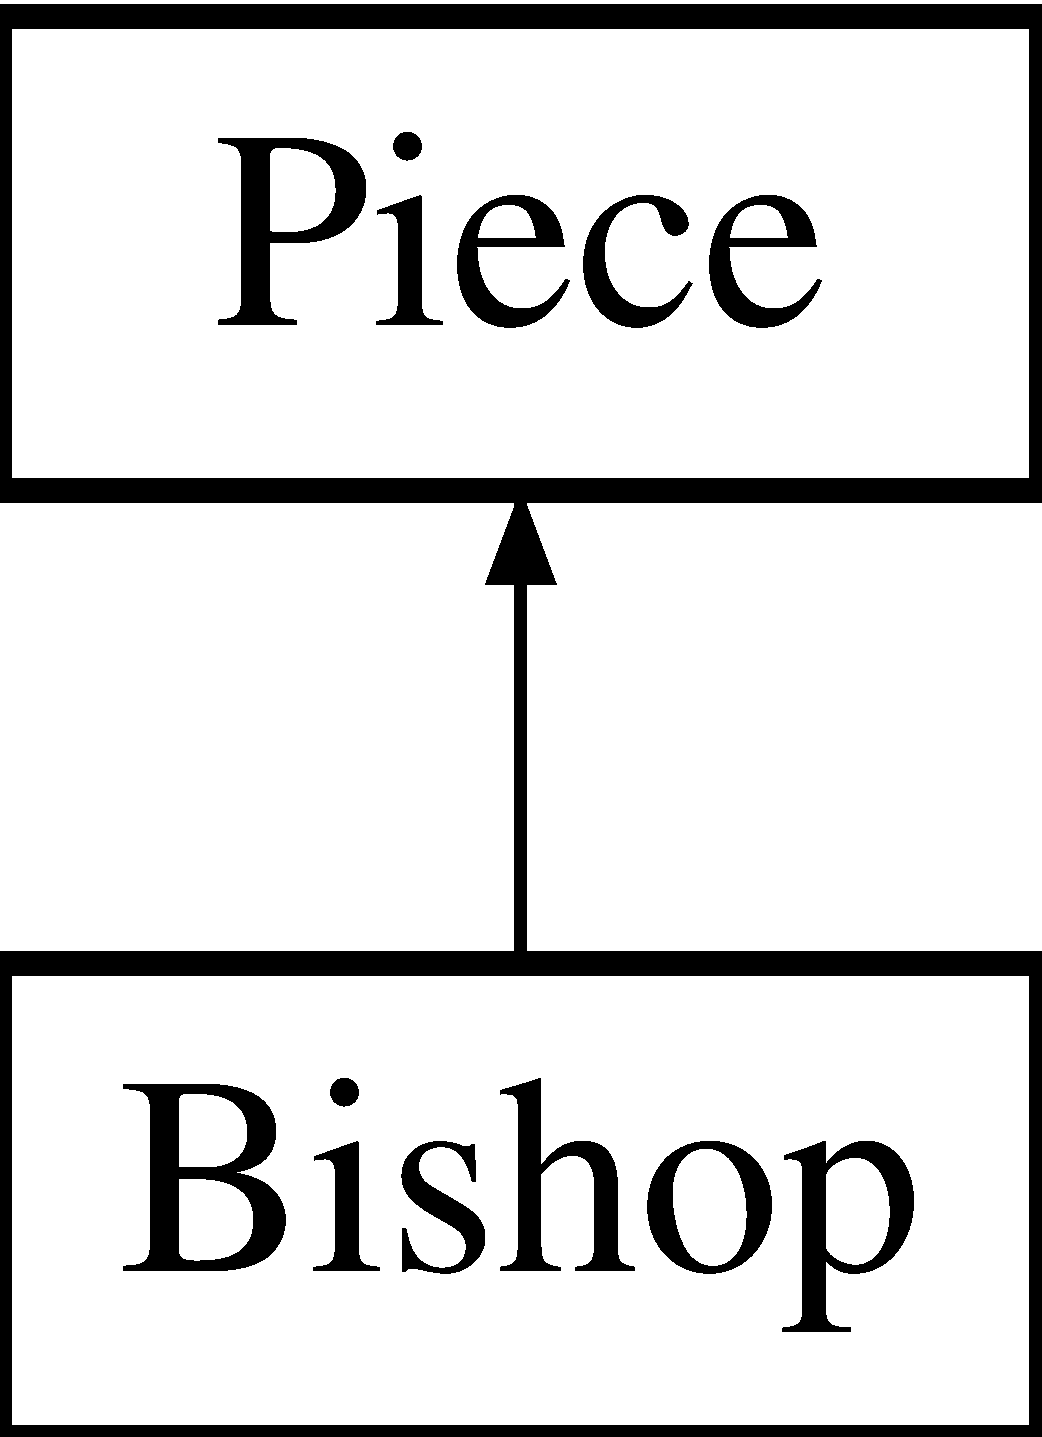
\includegraphics[height=2.000000cm]{class_bishop}
\end{center}
\end{figure}
\subsection*{Fonctions membres publiques}
\begin{DoxyCompactItemize}
\item 
\hyperlink{class_bishop_a7e73da51fcaac88ce0d16e78221142ee}{Bishop} (unsigned int x, unsigned int y)
\begin{DoxyCompactList}\small\item\em Constructeur, crée un objet \hyperlink{class_bishop}{Bishop} de coordonnées x,y. \end{DoxyCompactList}\item 
\hyperlink{class_bishop_a3705b4537a39d09a59143fe01a62442f}{$\sim$\-Bishop} ()
\begin{DoxyCompactList}\small\item\em Destructeur d'un objet cavalier. \end{DoxyCompactList}\item 
virtual void \hyperlink{class_bishop_abd25da5816a737ab64880cbaa7bd7582}{movement} ()
\begin{DoxyCompactList}\small\item\em procédure virtuelle permettant de mettre à jour l'attribut movements en fonction des déplacements possibles du Fou \end{DoxyCompactList}\end{DoxyCompactItemize}
\subsection*{Membres hérités additionnels}


\subsection{Description détaillée}
Classe \hyperlink{class_bishop}{Bishop} héritant de \hyperlink{class_piece}{Piece}. 

\subsection{Documentation des constructeurs et destructeur}
\hypertarget{class_bishop_a7e73da51fcaac88ce0d16e78221142ee}{\index{Bishop@{Bishop}!Bishop@{Bishop}}
\index{Bishop@{Bishop}!Bishop@{Bishop}}
\subsubsection[{Bishop}]{\setlength{\rightskip}{0pt plus 5cm}Bishop\-::\-Bishop (
\begin{DoxyParamCaption}
\item[{unsigned int}]{x, }
\item[{unsigned int}]{y}
\end{DoxyParamCaption}
)}}\label{class_bishop_a7e73da51fcaac88ce0d16e78221142ee}


Constructeur, crée un objet \hyperlink{class_bishop}{Bishop} de coordonnées x,y. 


\begin{DoxyParams}{Paramètres}
{\em unsigned} & int x \\
\hline
{\em unsigned} & int y \\
\hline
\end{DoxyParams}
\hypertarget{class_bishop_a3705b4537a39d09a59143fe01a62442f}{\index{Bishop@{Bishop}!$\sim$\-Bishop@{$\sim$\-Bishop}}
\index{$\sim$\-Bishop@{$\sim$\-Bishop}!Bishop@{Bishop}}
\subsubsection[{$\sim$\-Bishop}]{\setlength{\rightskip}{0pt plus 5cm}Bishop\-::$\sim$\-Bishop (
\begin{DoxyParamCaption}
{}
\end{DoxyParamCaption}
)}}\label{class_bishop_a3705b4537a39d09a59143fe01a62442f}


Destructeur d'un objet cavalier. 



\subsection{Documentation des fonctions membres}
\hypertarget{class_bishop_abd25da5816a737ab64880cbaa7bd7582}{\index{Bishop@{Bishop}!movement@{movement}}
\index{movement@{movement}!Bishop@{Bishop}}
\subsubsection[{movement}]{\setlength{\rightskip}{0pt plus 5cm}void Bishop\-::movement (
\begin{DoxyParamCaption}
{}
\end{DoxyParamCaption}
)\hspace{0.3cm}{\ttfamily [virtual]}}}\label{class_bishop_abd25da5816a737ab64880cbaa7bd7582}


procédure virtuelle permettant de mettre à jour l'attribut movements en fonction des déplacements possibles du Fou 



Réimplémentée à partir de \hyperlink{class_piece_ae721b5ed94376fd4e7d348d36739ed4d}{Piece}.



La documentation de cette classe a été générée à partir des fichiers suivants \-:\begin{DoxyCompactItemize}
\item 
src/\hyperlink{_piece_8hpp}{Piece.\-hpp}\item 
src/\hyperlink{_piece_8cpp}{Piece.\-cpp}\end{DoxyCompactItemize}

\hypertarget{class_cell}{\section{Référence de la classe Cell}
\label{class_cell}\index{Cell@{Cell}}
}


Classe permettant de représenter une case du jeu d'echec.  




{\ttfamily \#include $<$Cell.\-hpp$>$}

\subsection*{Fonctions membres publiques}
\begin{DoxyCompactItemize}
\item 
\hyperlink{class_cell_a4ccfb0a9923271daba6000afa1a33ee9}{Cell} (unsigned int x, unsigned int y)
\begin{DoxyCompactList}\small\item\em Constructeur, crée un objet \hyperlink{class_cell}{Cell} initialisant les coordonnées. \end{DoxyCompactList}\item 
\hyperlink{class_cell_a9fa559f7a28e2b4336c6879ca09304d8}{$\sim$\-Cell} ()
\begin{DoxyCompactList}\small\item\em Destructeur d'un objet \hyperlink{class_cell}{Cell}. \end{DoxyCompactList}\item 
unsigned int \hyperlink{class_cell_a09a86af000a7b6b00be01c0ea71e5319}{get\-X} ()
\begin{DoxyCompactList}\small\item\em Getter de l'attribut \-\_\-x. \end{DoxyCompactList}\item 
void \hyperlink{class_cell_a5db21f79684f86d4dad8e17a40bbb797}{set\-X} (unsigned int new\-X)
\begin{DoxyCompactList}\small\item\em Setter de l'attribut \-\_\-x. \end{DoxyCompactList}\item 
unsigned int \hyperlink{class_cell_a54bd0f63ff375abde26902cc2ca7ea78}{get\-Y} ()
\begin{DoxyCompactList}\small\item\em Getter de l'attribut \-\_\-y. \end{DoxyCompactList}\item 
void \hyperlink{class_cell_ad797a4c776783b15f4637b1f667f56a5}{set\-Y} (unsigned int new\-Y)
\begin{DoxyCompactList}\small\item\em Setter de l'attribut \-\_\-y. \end{DoxyCompactList}\item 
bool \hyperlink{class_cell_ae889f79cafc3dda80d430980e4418333}{operator==} (\hyperlink{class_cell}{Cell} \&c2)
\begin{DoxyCompactList}\small\item\em comparer avec une autre piece \end{DoxyCompactList}\end{DoxyCompactItemize}


\subsection{Description détaillée}
Classe permettant de représenter une case du jeu d'echec. 

Classe permettant de représenter une \hyperlink{class_team}{Team}. 

\subsection{Documentation des constructeurs et destructeur}
\hypertarget{class_cell_a4ccfb0a9923271daba6000afa1a33ee9}{\index{Cell@{Cell}!Cell@{Cell}}
\index{Cell@{Cell}!Cell@{Cell}}
\subsubsection[{Cell}]{\setlength{\rightskip}{0pt plus 5cm}Cell\-::\-Cell (
\begin{DoxyParamCaption}
\item[{unsigned int}]{x, }
\item[{unsigned int}]{y}
\end{DoxyParamCaption}
)}}\label{class_cell_a4ccfb0a9923271daba6000afa1a33ee9}


Constructeur, crée un objet \hyperlink{class_cell}{Cell} initialisant les coordonnées. 


\begin{DoxyParams}{Paramètres}
{\em unsigned} & int, x \\
\hline
{\em unsigned} & int, y \\
\hline
\end{DoxyParams}
\hypertarget{class_cell_a9fa559f7a28e2b4336c6879ca09304d8}{\index{Cell@{Cell}!$\sim$\-Cell@{$\sim$\-Cell}}
\index{$\sim$\-Cell@{$\sim$\-Cell}!Cell@{Cell}}
\subsubsection[{$\sim$\-Cell}]{\setlength{\rightskip}{0pt plus 5cm}Cell\-::$\sim$\-Cell (
\begin{DoxyParamCaption}
{}
\end{DoxyParamCaption}
)}}\label{class_cell_a9fa559f7a28e2b4336c6879ca09304d8}


Destructeur d'un objet \hyperlink{class_cell}{Cell}. 



\subsection{Documentation des fonctions membres}
\hypertarget{class_cell_a09a86af000a7b6b00be01c0ea71e5319}{\index{Cell@{Cell}!get\-X@{get\-X}}
\index{get\-X@{get\-X}!Cell@{Cell}}
\subsubsection[{get\-X}]{\setlength{\rightskip}{0pt plus 5cm}unsigned int Cell\-::get\-X (
\begin{DoxyParamCaption}
{}
\end{DoxyParamCaption}
)}}\label{class_cell_a09a86af000a7b6b00be01c0ea71e5319}


Getter de l'attribut \-\_\-x. 

\begin{DoxyReturn}{Renvoie}
attribut \-\_\-x 
\end{DoxyReturn}
\hypertarget{class_cell_a54bd0f63ff375abde26902cc2ca7ea78}{\index{Cell@{Cell}!get\-Y@{get\-Y}}
\index{get\-Y@{get\-Y}!Cell@{Cell}}
\subsubsection[{get\-Y}]{\setlength{\rightskip}{0pt plus 5cm}unsigned int Cell\-::get\-Y (
\begin{DoxyParamCaption}
{}
\end{DoxyParamCaption}
)}}\label{class_cell_a54bd0f63ff375abde26902cc2ca7ea78}


Getter de l'attribut \-\_\-y. 

\begin{DoxyReturn}{Renvoie}
attribut \-\_\-y 
\end{DoxyReturn}
\hypertarget{class_cell_ae889f79cafc3dda80d430980e4418333}{\index{Cell@{Cell}!operator==@{operator==}}
\index{operator==@{operator==}!Cell@{Cell}}
\subsubsection[{operator==}]{\setlength{\rightskip}{0pt plus 5cm}bool Cell\-::operator== (
\begin{DoxyParamCaption}
\item[{{\bf Cell} \&}]{c2}
\end{DoxyParamCaption}
)}}\label{class_cell_ae889f79cafc3dda80d430980e4418333}


comparer avec une autre piece 


\begin{DoxyParams}{Paramètres}
{\em unsigned} & cell newcell \\
\hline
\end{DoxyParams}
\hypertarget{class_cell_a5db21f79684f86d4dad8e17a40bbb797}{\index{Cell@{Cell}!set\-X@{set\-X}}
\index{set\-X@{set\-X}!Cell@{Cell}}
\subsubsection[{set\-X}]{\setlength{\rightskip}{0pt plus 5cm}void Cell\-::set\-X (
\begin{DoxyParamCaption}
\item[{unsigned int}]{new\-X}
\end{DoxyParamCaption}
)}}\label{class_cell_a5db21f79684f86d4dad8e17a40bbb797}


Setter de l'attribut \-\_\-x. 


\begin{DoxyParams}{Paramètres}
{\em unsigned} & int new\-X \\
\hline
\end{DoxyParams}
\hypertarget{class_cell_ad797a4c776783b15f4637b1f667f56a5}{\index{Cell@{Cell}!set\-Y@{set\-Y}}
\index{set\-Y@{set\-Y}!Cell@{Cell}}
\subsubsection[{set\-Y}]{\setlength{\rightskip}{0pt plus 5cm}void Cell\-::set\-Y (
\begin{DoxyParamCaption}
\item[{unsigned int}]{new\-Y}
\end{DoxyParamCaption}
)}}\label{class_cell_ad797a4c776783b15f4637b1f667f56a5}


Setter de l'attribut \-\_\-y. 


\begin{DoxyParams}{Paramètres}
{\em unsigned} & int new\-Y \\
\hline
\end{DoxyParams}


La documentation de cette classe a été générée à partir des fichiers suivants \-:\begin{DoxyCompactItemize}
\item 
src/\hyperlink{_cell_8hpp}{Cell.\-hpp}\item 
src/\hyperlink{_cell_8cpp}{Cell.\-cpp}\end{DoxyCompactItemize}

\hypertarget{class_check_state}{\section{Référence de la classe Check\-State}
\label{class_check_state}\index{Check\-State@{Check\-State}}
}


{\ttfamily \#include $<$State.\-hpp$>$}

Graphe d'héritage de Check\-State\-:\begin{figure}[H]
\begin{center}
\leavevmode
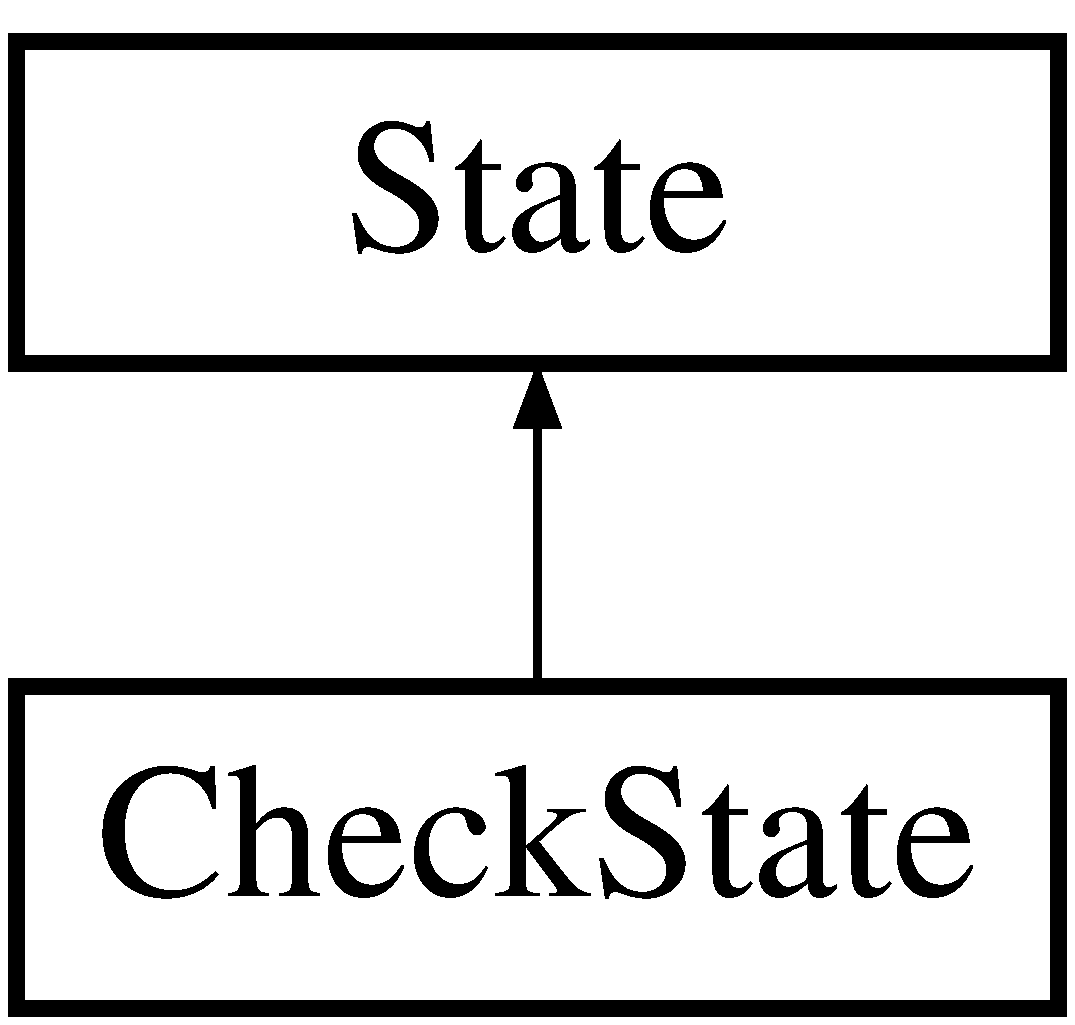
\includegraphics[height=2.000000cm]{class_check_state}
\end{center}
\end{figure}
\subsection*{Fonctions membres publiques}
\begin{DoxyCompactItemize}
\item 
\hyperlink{class_check_state_a5027a0f3dc626241c48ac33b0b974311}{Check\-State} (\hyperlink{class_player}{Player} $\ast$p)
\begin{DoxyCompactList}\small\item\em Constructeur, crée un Etat\-Echec à l'aide du constructeur de \hyperlink{class_state}{State} avec un Joueur en paramètre. \end{DoxyCompactList}\item 
\hyperlink{class_check_state_aecd4b3d189f47df10445e70aec28502b}{$\sim$\-Check\-State} ()
\begin{DoxyCompactList}\small\item\em Destructeur de l'objet \hyperlink{class_check_state}{Check\-State}. \end{DoxyCompactList}\item 
void \hyperlink{class_check_state_a3cc0cb64d061a72d91ee60b60801aa3b}{in\-Game} ()
\begin{DoxyCompactList}\small\item\em Définition de la procédure virtuelle, transition vers l'état \hyperlink{class_game_state}{Game\-State}. \end{DoxyCompactList}\item 
void \hyperlink{class_check_state_a7e365f95e322b61609f05202c28db278}{check} ()
\begin{DoxyCompactList}\small\item\em Définition de la procédure virtuelle, pas d'effet dans cet Etat là \end{DoxyCompactList}\item 
void \hyperlink{class_check_state_afb093377619bc04bcba50db601368019}{check\-Mate} ()
\begin{DoxyCompactList}\small\item\em Définition de la procédure virtuelle, pas d'effet dans cet Etat là \end{DoxyCompactList}\item 
void \hyperlink{class_check_state_ae3cc6446e2dd5de333797bb180104c50}{game\-Null} ()
\begin{DoxyCompactList}\small\item\em Définition de la procédure virtuelle, pas d'effet dans cet Etat là \end{DoxyCompactList}\item 
void \hyperlink{class_check_state_a54820bb890cc50e3782104fad094747f}{game\-End} ()
\begin{DoxyCompactList}\small\item\em Définition de la procédure virtuelle, pas d'effet dans cet Etat là \end{DoxyCompactList}\item 
void \hyperlink{class_check_state_ace4965a79b3614c50d0db5396121b75e}{print} ()
\begin{DoxyCompactList}\small\item\em Définition de la procédure virtuelle, affiche l'état \hyperlink{class_check_state}{Check\-State}. \end{DoxyCompactList}\item 
bool \hyperlink{class_check_state_aa6e88c453114883d8a415ff338b65526}{ischeck} ()
\begin{DoxyCompactList}\small\item\em procédure virtuelle permettant de savoir s'il se trouve en possition d'echec \end{DoxyCompactList}\item 
bool \hyperlink{class_check_state_ae3704aaa5fbaf6c947462c211eafc9c9}{ischeckmate} ()
\begin{DoxyCompactList}\small\item\em procédure virtuelle permettant de savoir s'il se trouve en possition d'echec et mat \end{DoxyCompactList}\item 
bool \hyperlink{class_check_state_a569daf96d0340272068a3d36fdf288c4}{isnulle} ()
\begin{DoxyCompactList}\small\item\em procédure virtuelle permettant de savoir s'il se trouve en possition nulle \end{DoxyCompactList}\end{DoxyCompactItemize}
\subsection*{Membres hérités additionnels}


\subsection{Documentation des constructeurs et destructeur}
\hypertarget{class_check_state_a5027a0f3dc626241c48ac33b0b974311}{\index{Check\-State@{Check\-State}!Check\-State@{Check\-State}}
\index{Check\-State@{Check\-State}!CheckState@{Check\-State}}
\subsubsection[{Check\-State}]{\setlength{\rightskip}{0pt plus 5cm}Check\-State\-::\-Check\-State (
\begin{DoxyParamCaption}
\item[{{\bf Player} $\ast$}]{p}
\end{DoxyParamCaption}
)}}\label{class_check_state_a5027a0f3dc626241c48ac33b0b974311}


Constructeur, crée un Etat\-Echec à l'aide du constructeur de \hyperlink{class_state}{State} avec un Joueur en paramètre. 


\begin{DoxyParams}{Paramètres}
{\em p} & \\
\hline
\end{DoxyParams}
\hypertarget{class_check_state_aecd4b3d189f47df10445e70aec28502b}{\index{Check\-State@{Check\-State}!$\sim$\-Check\-State@{$\sim$\-Check\-State}}
\index{$\sim$\-Check\-State@{$\sim$\-Check\-State}!CheckState@{Check\-State}}
\subsubsection[{$\sim$\-Check\-State}]{\setlength{\rightskip}{0pt plus 5cm}Check\-State\-::$\sim$\-Check\-State (
\begin{DoxyParamCaption}
{}
\end{DoxyParamCaption}
)}}\label{class_check_state_aecd4b3d189f47df10445e70aec28502b}


Destructeur de l'objet \hyperlink{class_check_state}{Check\-State}. 



\subsection{Documentation des fonctions membres}
\hypertarget{class_check_state_a7e365f95e322b61609f05202c28db278}{\index{Check\-State@{Check\-State}!check@{check}}
\index{check@{check}!CheckState@{Check\-State}}
\subsubsection[{check}]{\setlength{\rightskip}{0pt plus 5cm}void Check\-State\-::check (
\begin{DoxyParamCaption}
{}
\end{DoxyParamCaption}
)\hspace{0.3cm}{\ttfamily [virtual]}}}\label{class_check_state_a7e365f95e322b61609f05202c28db278}


Définition de la procédure virtuelle, pas d'effet dans cet Etat là 



Implémente \hyperlink{class_state_a321fd726bbefc35fedbbf001d2a37021}{State}.

\hypertarget{class_check_state_afb093377619bc04bcba50db601368019}{\index{Check\-State@{Check\-State}!check\-Mate@{check\-Mate}}
\index{check\-Mate@{check\-Mate}!CheckState@{Check\-State}}
\subsubsection[{check\-Mate}]{\setlength{\rightskip}{0pt plus 5cm}void Check\-State\-::check\-Mate (
\begin{DoxyParamCaption}
{}
\end{DoxyParamCaption}
)\hspace{0.3cm}{\ttfamily [virtual]}}}\label{class_check_state_afb093377619bc04bcba50db601368019}


Définition de la procédure virtuelle, pas d'effet dans cet Etat là 



Implémente \hyperlink{class_state_aa2b89ec92ecd4f6271269fe4b8ccc790}{State}.

\hypertarget{class_check_state_a54820bb890cc50e3782104fad094747f}{\index{Check\-State@{Check\-State}!game\-End@{game\-End}}
\index{game\-End@{game\-End}!CheckState@{Check\-State}}
\subsubsection[{game\-End}]{\setlength{\rightskip}{0pt plus 5cm}void Check\-State\-::game\-End (
\begin{DoxyParamCaption}
{}
\end{DoxyParamCaption}
)\hspace{0.3cm}{\ttfamily [virtual]}}}\label{class_check_state_a54820bb890cc50e3782104fad094747f}


Définition de la procédure virtuelle, pas d'effet dans cet Etat là 



Implémente \hyperlink{class_state_a5117e1f9bf06e17b4b0277838fe39bd8}{State}.

\hypertarget{class_check_state_ae3cc6446e2dd5de333797bb180104c50}{\index{Check\-State@{Check\-State}!game\-Null@{game\-Null}}
\index{game\-Null@{game\-Null}!CheckState@{Check\-State}}
\subsubsection[{game\-Null}]{\setlength{\rightskip}{0pt plus 5cm}void Check\-State\-::game\-Null (
\begin{DoxyParamCaption}
{}
\end{DoxyParamCaption}
)\hspace{0.3cm}{\ttfamily [virtual]}}}\label{class_check_state_ae3cc6446e2dd5de333797bb180104c50}


Définition de la procédure virtuelle, pas d'effet dans cet Etat là 



Implémente \hyperlink{class_state_ad5b7fe10b2c30243f36d7d0950c50d43}{State}.

\hypertarget{class_check_state_a3cc0cb64d061a72d91ee60b60801aa3b}{\index{Check\-State@{Check\-State}!in\-Game@{in\-Game}}
\index{in\-Game@{in\-Game}!CheckState@{Check\-State}}
\subsubsection[{in\-Game}]{\setlength{\rightskip}{0pt plus 5cm}void Check\-State\-::in\-Game (
\begin{DoxyParamCaption}
{}
\end{DoxyParamCaption}
)\hspace{0.3cm}{\ttfamily [virtual]}}}\label{class_check_state_a3cc0cb64d061a72d91ee60b60801aa3b}


Définition de la procédure virtuelle, transition vers l'état \hyperlink{class_game_state}{Game\-State}. 



Implémente \hyperlink{class_state_a738b04d6e0c12a39bf96a2a7159202d8}{State}.

\hypertarget{class_check_state_aa6e88c453114883d8a415ff338b65526}{\index{Check\-State@{Check\-State}!ischeck@{ischeck}}
\index{ischeck@{ischeck}!CheckState@{Check\-State}}
\subsubsection[{ischeck}]{\setlength{\rightskip}{0pt plus 5cm}bool Check\-State\-::ischeck (
\begin{DoxyParamCaption}
{}
\end{DoxyParamCaption}
)\hspace{0.3cm}{\ttfamily [virtual]}}}\label{class_check_state_aa6e88c453114883d8a415ff338b65526}


procédure virtuelle permettant de savoir s'il se trouve en possition d'echec 



Implémente \hyperlink{class_state_ad2d7084c507d8d20be2e772d953129fb}{State}.

\hypertarget{class_check_state_ae3704aaa5fbaf6c947462c211eafc9c9}{\index{Check\-State@{Check\-State}!ischeckmate@{ischeckmate}}
\index{ischeckmate@{ischeckmate}!CheckState@{Check\-State}}
\subsubsection[{ischeckmate}]{\setlength{\rightskip}{0pt plus 5cm}bool Check\-State\-::ischeckmate (
\begin{DoxyParamCaption}
{}
\end{DoxyParamCaption}
)\hspace{0.3cm}{\ttfamily [virtual]}}}\label{class_check_state_ae3704aaa5fbaf6c947462c211eafc9c9}


procédure virtuelle permettant de savoir s'il se trouve en possition d'echec et mat 



Implémente \hyperlink{class_state_ae1d813f250db75015ddeebece5ec0f2b}{State}.

\hypertarget{class_check_state_a569daf96d0340272068a3d36fdf288c4}{\index{Check\-State@{Check\-State}!isnulle@{isnulle}}
\index{isnulle@{isnulle}!CheckState@{Check\-State}}
\subsubsection[{isnulle}]{\setlength{\rightskip}{0pt plus 5cm}bool Check\-State\-::isnulle (
\begin{DoxyParamCaption}
{}
\end{DoxyParamCaption}
)\hspace{0.3cm}{\ttfamily [virtual]}}}\label{class_check_state_a569daf96d0340272068a3d36fdf288c4}


procédure virtuelle permettant de savoir s'il se trouve en possition nulle 



Implémente \hyperlink{class_state_a869f2ebfad7e60719df5f89a613adee1}{State}.

\hypertarget{class_check_state_ace4965a79b3614c50d0db5396121b75e}{\index{Check\-State@{Check\-State}!print@{print}}
\index{print@{print}!CheckState@{Check\-State}}
\subsubsection[{print}]{\setlength{\rightskip}{0pt plus 5cm}void Check\-State\-::print (
\begin{DoxyParamCaption}
{}
\end{DoxyParamCaption}
)\hspace{0.3cm}{\ttfamily [virtual]}}}\label{class_check_state_ace4965a79b3614c50d0db5396121b75e}


Définition de la procédure virtuelle, affiche l'état \hyperlink{class_check_state}{Check\-State}. 



Implémente \hyperlink{class_state_a95a537bb55b9118b23d5bed88ba3b335}{State}.



La documentation de cette classe a été générée à partir des fichiers suivants \-:\begin{DoxyCompactItemize}
\item 
src/\hyperlink{_state_8hpp}{State.\-hpp}\item 
src/\hyperlink{_state_8cpp}{State.\-cpp}\end{DoxyCompactItemize}

\hypertarget{class_chess}{\section{Référence de la classe Chess}
\label{class_chess}\index{Chess@{Chess}}
}


{\ttfamily \#include $<$Chess.\-hpp$>$}

\subsection*{Fonctions membres publiques}
\begin{DoxyCompactItemize}
\item 
\hyperlink{class_chess_a7524da0608df5a385dfd25d23d2d4e50}{Chess} (std\-::string name\-P1, std\-::string name\-P2)
\begin{DoxyCompactList}\small\item\em Constructeur, crée un objet \hyperlink{class_chess}{Chess}. \end{DoxyCompactList}\item 
\hyperlink{class_chess_aa9717ab5263bc4fbb844e78bbe5587a8}{$\sim$\-Chess} ()
\begin{DoxyCompactList}\small\item\em Destructeur de \hyperlink{class_chess}{Chess}. \end{DoxyCompactList}\item 
void \hyperlink{class_chess_a8fc79b0c34c21d522abd9b8ae62ee38f}{init\-Board} ()
\begin{DoxyCompactList}\small\item\em Initialise le plateau de jeu. \end{DoxyCompactList}\item 
\hyperlink{class_piece}{Piece} $\ast$ \hyperlink{class_chess_a67069ea8ee1fce34961fc9c645c4dc10}{select\-Dest} (\hyperlink{class_player}{Player} $\ast$player, \hyperlink{class_piece}{Piece} $\ast$piece, unsigned int x, unsigned int y)
\begin{DoxyCompactList}\small\item\em Permet au joueur de selectionner une destination pour son déplacement de pièce. \end{DoxyCompactList}\item 
bool \hyperlink{class_chess_ac29b7a4bed77102b3ddaf079ce2c9abf}{no\-Collision} (\hyperlink{class_piece}{Piece} $\ast$selected\-P, \hyperlink{class_piece}{Piece} $\ast$selected\-D, \hyperlink{class_piece}{Piece} $\ast$pieceaeviter, \hyperlink{class_piece}{Piece} $\ast$piece\-D)
\begin{DoxyCompactList}\small\item\em Vérifie s'il n'y a pas de collision lors du déplacement de la pièce vers la destination sélectionée. \end{DoxyCompactList}\item 
void \hyperlink{class_chess_aec36eadf1a550d2f6c85ec8a23bac2d1}{move\-Piece} (\hyperlink{class_piece}{Piece} $\ast$selected\-P, \hyperlink{class_piece}{Piece} $\ast$selected\-D)
\begin{DoxyCompactList}\small\item\em Effectue le déplacement de la pièce selectionnée vers la destination. \end{DoxyCompactList}\item 
bool \hyperlink{class_chess_ac521e181e266322da1664977b102afc5}{game\-Round} (\hyperlink{class_player}{Player} $\ast$player\-I\-G, \hyperlink{class_player}{Player} $\ast$adver)
\begin{DoxyCompactList}\small\item\em Effectue le tour d'un joueur. \end{DoxyCompactList}\item 
unsigned int \hyperlink{class_chess_a7d4dbb556159e245fe753d5a6daada8b}{get\-Choice\-Int} ()
\begin{DoxyCompactList}\small\item\em Permet l'entrée utilisateur d'une coordonnée valide. \end{DoxyCompactList}\item 
void \hyperlink{class_chess_a9cd677e16f4c08ddcdad57a4e12be99f}{print\-Board} ()
\begin{DoxyCompactList}\small\item\em Affiche le plateau dans le terminal. \end{DoxyCompactList}\item 
bool \hyperlink{class_chess_aae6464a0576a72f63aab8450b18dd580}{test\-Echec} (\hyperlink{class_player}{Player} $\ast$player\-I\-G, \hyperlink{class_player}{Player} $\ast$adver)
\begin{DoxyCompactList}\small\item\em Permet de savoir si un joueur se trouve en position d'echec. \end{DoxyCompactList}\item 
bool \hyperlink{class_chess_a1b5cf39c4f616e5e79bd16d4837bc2dc}{test\-Echec} (\hyperlink{class_piece}{Piece} $\ast$selected\-P, \hyperlink{class_player}{Player} $\ast$adver)
\begin{DoxyCompactList}\small\item\em Permet de savoir si une piece se trouve en position d'echec. \end{DoxyCompactList}\item 
bool \hyperlink{class_chess_a591da78c202b3e870c683789662a65c4}{test\-Echec\-Mat} (\hyperlink{class_player}{Player} $\ast$player\-I\-G, \hyperlink{class_player}{Player} $\ast$adver)
\begin{DoxyCompactList}\small\item\em Permet de savoir si un joueur se trouve en position d'echec et mat. \end{DoxyCompactList}\item 
bool \hyperlink{class_chess_a7b2dde25a7cbe133dbb0fa9e71909e8f}{on\-The\-Way} (\hyperlink{class_player}{Player} $\ast$player\-I\-G, \hyperlink{class_piece}{Piece} $\ast$piece\-D, \hyperlink{class_player}{Player} $\ast$advers)
\begin{DoxyCompactList}\small\item\em Permet de savoir si la piece\-D est sur le passage de la piece qui peut manger le roi. \end{DoxyCompactList}\item 
std\-::vector$<$ \hyperlink{class_piece}{Piece} $\ast$ $>$ \hyperlink{class_chess_ac70f9b16162244c5ab75e93b52db2024}{list\-Pieces} (\hyperlink{class_piece}{Piece} $\ast$selected\-P, \hyperlink{class_player}{Player} $\ast$advers)
\begin{DoxyCompactList}\small\item\em Permet de retourner une liste de pieces de l'advers qui peut manger la piece selected\-P. \end{DoxyCompactList}\item 
bool \hyperlink{class_chess_a860115fe5245b5d361ccb3ce7ea545b6}{list\-Can\-Eat\-King} (std\-::vector$<$ \hyperlink{class_piece}{Piece} $\ast$ $>$ list, \hyperlink{class_player}{Player} $\ast$advers, \hyperlink{class_player}{Player} $\ast$player\-I\-G, \hyperlink{class_piece}{Piece} $\ast$selected\-P, \hyperlink{class_piece}{Piece} $\ast$selected\-D)
\begin{DoxyCompactList}\small\item\em Permet de retourner un bool si une des pieces que peut manger la piece selected peut aller manger le roi du player\-I\-G si la piece selected\-P bouge. \end{DoxyCompactList}\item 
void \hyperlink{class_chess_a29329920258b662de0bdac41ba547f57}{transfo\-Spawn} (\hyperlink{class_player}{Player} $\ast$player\-I\-G, \hyperlink{class_piece}{Piece} $\ast$selected\-P, \hyperlink{class_piece}{Piece} $\ast$selected\-D)
\begin{DoxyCompactList}\small\item\em Procédure permettant de transformer le spawn. \end{DoxyCompactList}\item 
bool \hyperlink{class_chess_a750a533ab68f71194b7f1ea7a0b5cdda}{try\-Castling} (\hyperlink{class_player}{Player} $\ast$player\-I\-G, \hyperlink{class_piece}{Piece} $\ast$selected\-P, \hyperlink{class_piece}{Piece} $\ast$selected\-D)
\begin{DoxyCompactList}\small\item\em fonction permettant de savoir si le petit roque est possible \end{DoxyCompactList}\item 
bool \hyperlink{class_chess_a63ef59d4f464e63ae2da3386c1abcea3}{try\-G\-Castling} (\hyperlink{class_player}{Player} $\ast$player\-I\-G, \hyperlink{class_piece}{Piece} $\ast$selected\-P, \hyperlink{class_piece}{Piece} $\ast$selected\-D)
\begin{DoxyCompactList}\small\item\em fonction permettant de savoir si le grand roque est possible \end{DoxyCompactList}\item 
void \hyperlink{class_chess_af1af4be28978dcf09309883d38cf71cd}{castling} (\hyperlink{class_player}{Player} $\ast$player\-I\-G)
\begin{DoxyCompactList}\small\item\em Procédure permettant de faire le petit roque. \end{DoxyCompactList}\item 
void \hyperlink{class_chess_a81042bba80e10e971474b6f8488d8242}{g\-Castling} (\hyperlink{class_player}{Player} $\ast$player\-I\-G)
\begin{DoxyCompactList}\small\item\em Procédure permettant de faire le grand roque. \end{DoxyCompactList}\item 
bool \hyperlink{class_chess_a003d9681123559dc1c1b665695e6cd20}{is\-Piece\-In} (\hyperlink{class_piece}{Piece} $\ast$piece, \hyperlink{class_player}{Player} $\ast$player\-I\-G)
\begin{DoxyCompactList}\small\item\em fonction permettant de savoir si une piece appartient au player I\-G \end{DoxyCompactList}\item 
bool \hyperlink{class_chess_a97adeb237c2acae0efe4097a36a304b9}{is\-Null} ()
\begin{DoxyCompactList}\small\item\em fonction permettant de savoir si la partie se trouve en partie nulle \end{DoxyCompactList}\item 
void \hyperlink{class_chess_aea92734ff5516066d5c1a690a78ea146}{start\-Game} ()
\begin{DoxyCompactList}\small\item\em Lance le début d'une partie. \end{DoxyCompactList}\end{DoxyCompactItemize}


\subsection{Documentation des constructeurs et destructeur}
\hypertarget{class_chess_a7524da0608df5a385dfd25d23d2d4e50}{\index{Chess@{Chess}!Chess@{Chess}}
\index{Chess@{Chess}!Chess@{Chess}}
\subsubsection[{Chess}]{\setlength{\rightskip}{0pt plus 5cm}Chess\-::\-Chess (
\begin{DoxyParamCaption}
\item[{std\-::string}]{name\-P1, }
\item[{std\-::string}]{name\-P2}
\end{DoxyParamCaption}
)}}\label{class_chess_a7524da0608df5a385dfd25d23d2d4e50}


Constructeur, crée un objet \hyperlink{class_chess}{Chess}. 


\begin{DoxyParams}{Paramètres}
{\em string} & name\-P1 \\
\hline
{\em string} & name\-P2 \\
\hline
\end{DoxyParams}
\hypertarget{class_chess_aa9717ab5263bc4fbb844e78bbe5587a8}{\index{Chess@{Chess}!$\sim$\-Chess@{$\sim$\-Chess}}
\index{$\sim$\-Chess@{$\sim$\-Chess}!Chess@{Chess}}
\subsubsection[{$\sim$\-Chess}]{\setlength{\rightskip}{0pt plus 5cm}Chess\-::$\sim$\-Chess (
\begin{DoxyParamCaption}
{}
\end{DoxyParamCaption}
)}}\label{class_chess_aa9717ab5263bc4fbb844e78bbe5587a8}


Destructeur de \hyperlink{class_chess}{Chess}. 



\subsection{Documentation des fonctions membres}
\hypertarget{class_chess_af1af4be28978dcf09309883d38cf71cd}{\index{Chess@{Chess}!castling@{castling}}
\index{castling@{castling}!Chess@{Chess}}
\subsubsection[{castling}]{\setlength{\rightskip}{0pt plus 5cm}void Chess\-::castling (
\begin{DoxyParamCaption}
\item[{{\bf Player} $\ast$}]{player\-I\-G}
\end{DoxyParamCaption}
)}}\label{class_chess_af1af4be28978dcf09309883d38cf71cd}


Procédure permettant de faire le petit roque. 


\begin{DoxyParams}{Paramètres}
{\em Player$\ast$} & player\-I\-G, joueur actuellement en jeu \\
\hline
\end{DoxyParams}
\hypertarget{class_chess_ac521e181e266322da1664977b102afc5}{\index{Chess@{Chess}!game\-Round@{game\-Round}}
\index{game\-Round@{game\-Round}!Chess@{Chess}}
\subsubsection[{game\-Round}]{\setlength{\rightskip}{0pt plus 5cm}bool Chess\-::game\-Round (
\begin{DoxyParamCaption}
\item[{{\bf Player} $\ast$}]{player\-I\-G, }
\item[{{\bf Player} $\ast$}]{adver}
\end{DoxyParamCaption}
)}}\label{class_chess_ac521e181e266322da1664977b102afc5}


Effectue le tour d'un joueur. 


\begin{DoxyParams}{Paramètres}
{\em Player$\ast$} & player\-I\-G, Joueur actuellement en jeu \\
\hline
{\em Player$\ast$} & adver, Joueur en attente de jouer \\
\hline
\end{DoxyParams}
\begin{DoxyReturn}{Renvoie}
bool ( true si le joueur veut arreter de joueur) 
\end{DoxyReturn}
\hypertarget{class_chess_a81042bba80e10e971474b6f8488d8242}{\index{Chess@{Chess}!g\-Castling@{g\-Castling}}
\index{g\-Castling@{g\-Castling}!Chess@{Chess}}
\subsubsection[{g\-Castling}]{\setlength{\rightskip}{0pt plus 5cm}void Chess\-::g\-Castling (
\begin{DoxyParamCaption}
\item[{{\bf Player} $\ast$}]{player\-I\-G}
\end{DoxyParamCaption}
)}}\label{class_chess_a81042bba80e10e971474b6f8488d8242}


Procédure permettant de faire le grand roque. 


\begin{DoxyParams}{Paramètres}
{\em Player$\ast$} & player\-I\-G, joueur actuellement en jeu \\
\hline
\end{DoxyParams}
\hypertarget{class_chess_a7d4dbb556159e245fe753d5a6daada8b}{\index{Chess@{Chess}!get\-Choice\-Int@{get\-Choice\-Int}}
\index{get\-Choice\-Int@{get\-Choice\-Int}!Chess@{Chess}}
\subsubsection[{get\-Choice\-Int}]{\setlength{\rightskip}{0pt plus 5cm}unsigned int Chess\-::get\-Choice\-Int (
\begin{DoxyParamCaption}
{}
\end{DoxyParamCaption}
)}}\label{class_chess_a7d4dbb556159e245fe753d5a6daada8b}


Permet l'entrée utilisateur d'une coordonnée valide. 

\begin{DoxyReturn}{Renvoie}
unsigned int, coordonnée comprise entre 0 et 7 
\end{DoxyReturn}
\hypertarget{class_chess_a8fc79b0c34c21d522abd9b8ae62ee38f}{\index{Chess@{Chess}!init\-Board@{init\-Board}}
\index{init\-Board@{init\-Board}!Chess@{Chess}}
\subsubsection[{init\-Board}]{\setlength{\rightskip}{0pt plus 5cm}void Chess\-::init\-Board (
\begin{DoxyParamCaption}
{}
\end{DoxyParamCaption}
)}}\label{class_chess_a8fc79b0c34c21d522abd9b8ae62ee38f}


Initialise le plateau de jeu. 

\hypertarget{class_chess_a97adeb237c2acae0efe4097a36a304b9}{\index{Chess@{Chess}!is\-Null@{is\-Null}}
\index{is\-Null@{is\-Null}!Chess@{Chess}}
\subsubsection[{is\-Null}]{\setlength{\rightskip}{0pt plus 5cm}bool Chess\-::is\-Null (
\begin{DoxyParamCaption}
{}
\end{DoxyParamCaption}
)}}\label{class_chess_a97adeb237c2acae0efe4097a36a304b9}


fonction permettant de savoir si la partie se trouve en partie nulle 

\begin{DoxyReturn}{Renvoie}
bool 
\end{DoxyReturn}
\hypertarget{class_chess_a003d9681123559dc1c1b665695e6cd20}{\index{Chess@{Chess}!is\-Piece\-In@{is\-Piece\-In}}
\index{is\-Piece\-In@{is\-Piece\-In}!Chess@{Chess}}
\subsubsection[{is\-Piece\-In}]{\setlength{\rightskip}{0pt plus 5cm}bool Chess\-::is\-Piece\-In (
\begin{DoxyParamCaption}
\item[{{\bf Piece} $\ast$}]{piece, }
\item[{{\bf Player} $\ast$}]{player\-I\-G}
\end{DoxyParamCaption}
)}}\label{class_chess_a003d9681123559dc1c1b665695e6cd20}


fonction permettant de savoir si une piece appartient au player I\-G 


\begin{DoxyParams}{Paramètres}
{\em Piece$\ast$} & piece, pointeur vers une piece \\
\hline
{\em Player$\ast$} & player\-I\-G, joueur actuellement en jeu \\
\hline
\end{DoxyParams}
\begin{DoxyReturn}{Renvoie}
bool 
\end{DoxyReturn}
\hypertarget{class_chess_a860115fe5245b5d361ccb3ce7ea545b6}{\index{Chess@{Chess}!list\-Can\-Eat\-King@{list\-Can\-Eat\-King}}
\index{list\-Can\-Eat\-King@{list\-Can\-Eat\-King}!Chess@{Chess}}
\subsubsection[{list\-Can\-Eat\-King}]{\setlength{\rightskip}{0pt plus 5cm}bool Chess\-::list\-Can\-Eat\-King (
\begin{DoxyParamCaption}
\item[{std\-::vector$<$ {\bf Piece} $\ast$ $>$}]{list, }
\item[{{\bf Player} $\ast$}]{advers, }
\item[{{\bf Player} $\ast$}]{player\-I\-G, }
\item[{{\bf Piece} $\ast$}]{selected\-P, }
\item[{{\bf Piece} $\ast$}]{selected\-D}
\end{DoxyParamCaption}
)}}\label{class_chess_a860115fe5245b5d361ccb3ce7ea545b6}


Permet de retourner un bool si une des pieces que peut manger la piece selected peut aller manger le roi du player\-I\-G si la piece selected\-P bouge. 


\begin{DoxyParams}{Paramètres}
{\em vector$<$\-Piece$\ast$$>$} & list, vecteur d'une liste de pièce \\
\hline
{\em Player$\ast$} & advers, joueur adversaire \\
\hline
{\em Player$\ast$} & player\-I\-G, joueur actuellement en jeu \\
\hline
{\em Piece$\ast$} & selected\-P, pointeur d'une piece \\
\hline
{\em Piece$\ast$} & selected\-D, pointeur d'une piece \\
\hline
\end{DoxyParams}
\begin{DoxyReturn}{Renvoie}
bool 
\end{DoxyReturn}
\hypertarget{class_chess_ac70f9b16162244c5ab75e93b52db2024}{\index{Chess@{Chess}!list\-Pieces@{list\-Pieces}}
\index{list\-Pieces@{list\-Pieces}!Chess@{Chess}}
\subsubsection[{list\-Pieces}]{\setlength{\rightskip}{0pt plus 5cm}std\-::vector$<$ {\bf Piece} $\ast$ $>$ Chess\-::list\-Pieces (
\begin{DoxyParamCaption}
\item[{{\bf Piece} $\ast$}]{selected\-P, }
\item[{{\bf Player} $\ast$}]{advers}
\end{DoxyParamCaption}
)}}\label{class_chess_ac70f9b16162244c5ab75e93b52db2024}


Permet de retourner une liste de pieces de l'advers qui peut manger la piece selected\-P. 


\begin{DoxyParams}{Paramètres}
{\em Piece$\ast$} & selected\-P, pointeur d'une piece \\
\hline
{\em Player$\ast$} & advers, joueur adversaire \\
\hline
\end{DoxyParams}
\begin{DoxyReturn}{Renvoie}
liste de piece 
\end{DoxyReturn}
\hypertarget{class_chess_aec36eadf1a550d2f6c85ec8a23bac2d1}{\index{Chess@{Chess}!move\-Piece@{move\-Piece}}
\index{move\-Piece@{move\-Piece}!Chess@{Chess}}
\subsubsection[{move\-Piece}]{\setlength{\rightskip}{0pt plus 5cm}void Chess\-::move\-Piece (
\begin{DoxyParamCaption}
\item[{{\bf Piece} $\ast$}]{selected\-P, }
\item[{{\bf Piece} $\ast$}]{selected\-D}
\end{DoxyParamCaption}
)}}\label{class_chess_aec36eadf1a550d2f6c85ec8a23bac2d1}


Effectue le déplacement de la pièce selectionnée vers la destination. 


\begin{DoxyParams}{Paramètres}
{\em Piece$\ast$} & selected\-P, pointeur vers la pièce selectionnée \\
\hline
{\em Piece$\ast$} & selected\-D, pointeur vers la pièce représentant la destination \\
\hline
\end{DoxyParams}
\hypertarget{class_chess_ac29b7a4bed77102b3ddaf079ce2c9abf}{\index{Chess@{Chess}!no\-Collision@{no\-Collision}}
\index{no\-Collision@{no\-Collision}!Chess@{Chess}}
\subsubsection[{no\-Collision}]{\setlength{\rightskip}{0pt plus 5cm}bool Chess\-::no\-Collision (
\begin{DoxyParamCaption}
\item[{{\bf Piece} $\ast$}]{selected\-P, }
\item[{{\bf Piece} $\ast$}]{selected\-D, }
\item[{{\bf Piece} $\ast$}]{pieceaeviter = {\ttfamily NULL}, }
\item[{{\bf Piece} $\ast$}]{piece\-D = {\ttfamily NULL}}
\end{DoxyParamCaption}
)}}\label{class_chess_ac29b7a4bed77102b3ddaf079ce2c9abf}


Vérifie s'il n'y a pas de collision lors du déplacement de la pièce vers la destination sélectionée. 


\begin{DoxyParams}{Paramètres}
{\em Piece$\ast$} & selected\-P, pointeur vers la pièce selectionnée \\
\hline
{\em Piece$\ast$} & selected\-D, pointeur vers la pièce représentant la destination \\
\hline
{\em Piece$\ast$} & pieceaeviter = N\-U\-L\-L, pointeur vers la pièce représentant une piece a éviter \\
\hline
{\em Piece$\ast$} & piece\-D = N\-U\-L\-L , pointeur vers la pièce représentant la destination virtuel\\
\hline
\end{DoxyParams}
\begin{DoxyReturn}{Renvoie}
bool, vrai s'il n'y a pas de collision, faux sinon 
\end{DoxyReturn}
\hypertarget{class_chess_a7b2dde25a7cbe133dbb0fa9e71909e8f}{\index{Chess@{Chess}!on\-The\-Way@{on\-The\-Way}}
\index{on\-The\-Way@{on\-The\-Way}!Chess@{Chess}}
\subsubsection[{on\-The\-Way}]{\setlength{\rightskip}{0pt plus 5cm}bool Chess\-::on\-The\-Way (
\begin{DoxyParamCaption}
\item[{{\bf Player} $\ast$}]{player\-I\-G, }
\item[{{\bf Piece} $\ast$}]{piece\-D, }
\item[{{\bf Player} $\ast$}]{advers}
\end{DoxyParamCaption}
)}}\label{class_chess_a7b2dde25a7cbe133dbb0fa9e71909e8f}


Permet de savoir si la piece\-D est sur le passage de la piece qui peut manger le roi. 


\begin{DoxyParams}{Paramètres}
{\em Player$\ast$} & player\-I\-G, joueur actuellement en jeu \\
\hline
{\em Piece$\ast$} & piece\-D, pointeur d'une piece qui sera une destination \\
\hline
{\em Player$\ast$} & advers, joueur adversaire \\
\hline
\end{DoxyParams}
\begin{DoxyReturn}{Renvoie}
bool 
\end{DoxyReturn}
\hypertarget{class_chess_a9cd677e16f4c08ddcdad57a4e12be99f}{\index{Chess@{Chess}!print\-Board@{print\-Board}}
\index{print\-Board@{print\-Board}!Chess@{Chess}}
\subsubsection[{print\-Board}]{\setlength{\rightskip}{0pt plus 5cm}void Chess\-::print\-Board (
\begin{DoxyParamCaption}
{}
\end{DoxyParamCaption}
)}}\label{class_chess_a9cd677e16f4c08ddcdad57a4e12be99f}


Affiche le plateau dans le terminal. 

\hypertarget{class_chess_a67069ea8ee1fce34961fc9c645c4dc10}{\index{Chess@{Chess}!select\-Dest@{select\-Dest}}
\index{select\-Dest@{select\-Dest}!Chess@{Chess}}
\subsubsection[{select\-Dest}]{\setlength{\rightskip}{0pt plus 5cm}{\bf Piece} $\ast$ Chess\-::select\-Dest (
\begin{DoxyParamCaption}
\item[{{\bf Player} $\ast$}]{player, }
\item[{{\bf Piece} $\ast$}]{piece, }
\item[{unsigned int}]{x, }
\item[{unsigned int}]{y}
\end{DoxyParamCaption}
)}}\label{class_chess_a67069ea8ee1fce34961fc9c645c4dc10}


Permet au joueur de selectionner une destination pour son déplacement de pièce. 


\begin{DoxyParams}{Paramètres}
{\em unsigned} & int x, coordonnée x de la case selectionnée \\
\hline
{\em unsigned} & int y, coordonnée y de la case selectionnée \\
\hline
{\em Player$\ast$} & player, pointeur vers le joueur en jeu \\
\hline
{\em Piece$\ast$} & piece, pointeur de la pièce que le joueur veut déplacer \\
\hline
\end{DoxyParams}
\begin{DoxyReturn}{Renvoie}
Piece$\ast$ pointeur de la destination selectionnée sur le plateau (le board étant un tableau de \hyperlink{class_piece}{Piece}) 
\end{DoxyReturn}
\hypertarget{class_chess_aea92734ff5516066d5c1a690a78ea146}{\index{Chess@{Chess}!start\-Game@{start\-Game}}
\index{start\-Game@{start\-Game}!Chess@{Chess}}
\subsubsection[{start\-Game}]{\setlength{\rightskip}{0pt plus 5cm}void Chess\-::start\-Game (
\begin{DoxyParamCaption}
{}
\end{DoxyParamCaption}
)}}\label{class_chess_aea92734ff5516066d5c1a690a78ea146}


Lance le début d'une partie. 

\hypertarget{class_chess_aae6464a0576a72f63aab8450b18dd580}{\index{Chess@{Chess}!test\-Echec@{test\-Echec}}
\index{test\-Echec@{test\-Echec}!Chess@{Chess}}
\subsubsection[{test\-Echec}]{\setlength{\rightskip}{0pt plus 5cm}bool Chess\-::test\-Echec (
\begin{DoxyParamCaption}
\item[{{\bf Player} $\ast$}]{player\-I\-G, }
\item[{{\bf Player} $\ast$}]{adver}
\end{DoxyParamCaption}
)}}\label{class_chess_aae6464a0576a72f63aab8450b18dd580}


Permet de savoir si un joueur se trouve en position d'echec. 


\begin{DoxyParams}{Paramètres}
{\em Player$\ast$} & player\-I\-G, joueur actuellement en jeu \\
\hline
{\em Player$\ast$} & adver, joueur adversaire \\
\hline
\end{DoxyParams}
\begin{DoxyReturn}{Renvoie}
bool 
\end{DoxyReturn}
\hypertarget{class_chess_a1b5cf39c4f616e5e79bd16d4837bc2dc}{\index{Chess@{Chess}!test\-Echec@{test\-Echec}}
\index{test\-Echec@{test\-Echec}!Chess@{Chess}}
\subsubsection[{test\-Echec}]{\setlength{\rightskip}{0pt plus 5cm}bool Chess\-::test\-Echec (
\begin{DoxyParamCaption}
\item[{{\bf Piece} $\ast$}]{selected\-P, }
\item[{{\bf Player} $\ast$}]{adver}
\end{DoxyParamCaption}
)}}\label{class_chess_a1b5cf39c4f616e5e79bd16d4837bc2dc}


Permet de savoir si une piece se trouve en position d'echec. 


\begin{DoxyParams}{Paramètres}
{\em Piece$\ast$} & player\-I\-G, pointeur d'une piece \\
\hline
{\em Player$\ast$} & adver, joueur adversaire \\
\hline
\end{DoxyParams}
\begin{DoxyReturn}{Renvoie}
bool 
\end{DoxyReturn}
\hypertarget{class_chess_a591da78c202b3e870c683789662a65c4}{\index{Chess@{Chess}!test\-Echec\-Mat@{test\-Echec\-Mat}}
\index{test\-Echec\-Mat@{test\-Echec\-Mat}!Chess@{Chess}}
\subsubsection[{test\-Echec\-Mat}]{\setlength{\rightskip}{0pt plus 5cm}bool Chess\-::test\-Echec\-Mat (
\begin{DoxyParamCaption}
\item[{{\bf Player} $\ast$}]{player\-I\-G, }
\item[{{\bf Player} $\ast$}]{adver}
\end{DoxyParamCaption}
)}}\label{class_chess_a591da78c202b3e870c683789662a65c4}


Permet de savoir si un joueur se trouve en position d'echec et mat. 


\begin{DoxyParams}{Paramètres}
{\em Player$\ast$} & player\-I\-G, joueur actuellement en jeu \\
\hline
{\em Player$\ast$} & adver, joueur adversaire \\
\hline
\end{DoxyParams}
\begin{DoxyReturn}{Renvoie}
bool 
\end{DoxyReturn}
\hypertarget{class_chess_a29329920258b662de0bdac41ba547f57}{\index{Chess@{Chess}!transfo\-Spawn@{transfo\-Spawn}}
\index{transfo\-Spawn@{transfo\-Spawn}!Chess@{Chess}}
\subsubsection[{transfo\-Spawn}]{\setlength{\rightskip}{0pt plus 5cm}void Chess\-::transfo\-Spawn (
\begin{DoxyParamCaption}
\item[{{\bf Player} $\ast$}]{player\-I\-G, }
\item[{{\bf Piece} $\ast$}]{selected\-P, }
\item[{{\bf Piece} $\ast$}]{selected\-D}
\end{DoxyParamCaption}
)}}\label{class_chess_a29329920258b662de0bdac41ba547f57}


Procédure permettant de transformer le spawn. 


\begin{DoxyParams}{Paramètres}
{\em Player$\ast$} & player\-I\-G, joueur actuellement en jeu \\
\hline
{\em Piece$\ast$} & selected\-P, pointeur d'une piece \\
\hline
{\em Piece$\ast$} & selected\-D, pointeur d'une piece \\
\hline
\end{DoxyParams}
\hypertarget{class_chess_a750a533ab68f71194b7f1ea7a0b5cdda}{\index{Chess@{Chess}!try\-Castling@{try\-Castling}}
\index{try\-Castling@{try\-Castling}!Chess@{Chess}}
\subsubsection[{try\-Castling}]{\setlength{\rightskip}{0pt plus 5cm}bool Chess\-::try\-Castling (
\begin{DoxyParamCaption}
\item[{{\bf Player} $\ast$}]{player\-I\-G, }
\item[{{\bf Piece} $\ast$}]{selected\-P, }
\item[{{\bf Piece} $\ast$}]{selected\-D}
\end{DoxyParamCaption}
)}}\label{class_chess_a750a533ab68f71194b7f1ea7a0b5cdda}


fonction permettant de savoir si le petit roque est possible 


\begin{DoxyParams}{Paramètres}
{\em Player$\ast$} & player\-I\-G, joueur actuellement en jeu \\
\hline
{\em Piece$\ast$} & selected\-P, pointeur d'une piece \\
\hline
{\em Piece$\ast$} & selected\-D, pointeur d'une piece \\
\hline
\end{DoxyParams}
\hypertarget{class_chess_a63ef59d4f464e63ae2da3386c1abcea3}{\index{Chess@{Chess}!try\-G\-Castling@{try\-G\-Castling}}
\index{try\-G\-Castling@{try\-G\-Castling}!Chess@{Chess}}
\subsubsection[{try\-G\-Castling}]{\setlength{\rightskip}{0pt plus 5cm}bool Chess\-::try\-G\-Castling (
\begin{DoxyParamCaption}
\item[{{\bf Player} $\ast$}]{player\-I\-G, }
\item[{{\bf Piece} $\ast$}]{selected\-P, }
\item[{{\bf Piece} $\ast$}]{selected\-D}
\end{DoxyParamCaption}
)}}\label{class_chess_a63ef59d4f464e63ae2da3386c1abcea3}


fonction permettant de savoir si le grand roque est possible 


\begin{DoxyParams}{Paramètres}
{\em Player$\ast$} & player\-I\-G, joueur actuellement en jeu \\
\hline
{\em Piece$\ast$} & selected\-P, pointeur d'une piece \\
\hline
{\em Piece$\ast$} & selected\-D, pointeur d'une piece \\
\hline
\end{DoxyParams}


La documentation de cette classe a été générée à partir des fichiers suivants \-:\begin{DoxyCompactItemize}
\item 
src/\hyperlink{_chess_8hpp}{Chess.\-hpp}\item 
src/\hyperlink{_chess_8cpp}{Chess.\-cpp}\end{DoxyCompactItemize}

\hypertarget{class_end_state}{\section{Référence de la classe End\-State}
\label{class_end_state}\index{End\-State@{End\-State}}
}


{\ttfamily \#include $<$State.\-hpp$>$}

Graphe d'héritage de End\-State\-:\begin{figure}[H]
\begin{center}
\leavevmode
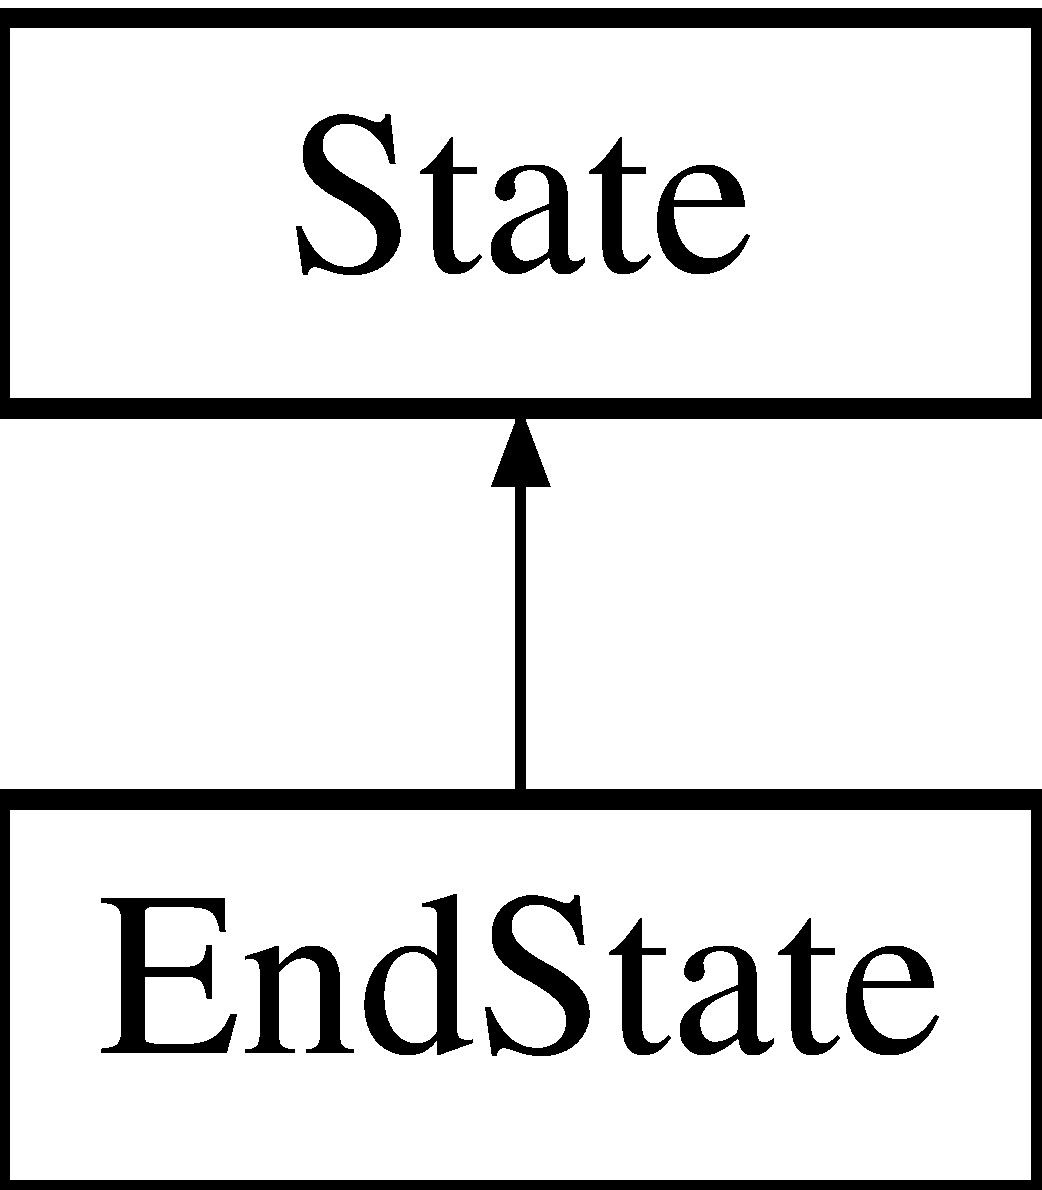
\includegraphics[height=2.000000cm]{class_end_state}
\end{center}
\end{figure}
\subsection*{Fonctions membres publiques}
\begin{DoxyCompactItemize}
\item 
\hyperlink{class_end_state_a0c74d371934fe30dd66ad3275b0ca98e}{End\-State} (\hyperlink{class_player}{Player} $\ast$p)
\begin{DoxyCompactList}\small\item\em Constructeur, crée un Etat\-Fin à l'aide du constructeur de \hyperlink{class_state}{State} avec un Joueur en paramètre. \end{DoxyCompactList}\item 
\hyperlink{class_end_state_a201636e52f201f6f34318c152139e2e1}{$\sim$\-End\-State} ()
\begin{DoxyCompactList}\small\item\em Destructeur de l'objet \hyperlink{class_end_state}{End\-State}. \end{DoxyCompactList}\item 
void \hyperlink{class_end_state_a6ba5aa5cfd2d0ac4aa1609e336d5669f}{in\-Game} ()
\begin{DoxyCompactList}\small\item\em Définition de la procédure virtuelle, pas d'effet dans cet Etat là \end{DoxyCompactList}\item 
void \hyperlink{class_end_state_a80e538c38c1293803200e5d3b513ba77}{check} ()
\begin{DoxyCompactList}\small\item\em Définition de la procédure virtuelle, pas d'effet dans cet Etat là \end{DoxyCompactList}\item 
void \hyperlink{class_end_state_a48a2531ee4bd2144b44823a5527488f3}{check\-Mate} ()
\begin{DoxyCompactList}\small\item\em Définition de la procédure virtuelle, pas d'effet dans cet Etat là \end{DoxyCompactList}\item 
void \hyperlink{class_end_state_ad50c108e27c7b0497c3f2f2e76b904a5}{game\-Null} ()
\begin{DoxyCompactList}\small\item\em Définition de la procédure virtuelle, pas d'effet dans cet Etat là \end{DoxyCompactList}\item 
void \hyperlink{class_end_state_a6fc13eb28853a79e1b5396dd2f377a51}{game\-End} ()
\begin{DoxyCompactList}\small\item\em Définition de la procédure virtuelle, pas d'effet dans cet Etat là \end{DoxyCompactList}\item 
void \hyperlink{class_end_state_a1983377ed8a1e391871fb40db39f13e3}{print} ()
\begin{DoxyCompactList}\small\item\em Définition de la procédure virtuelle, affiche l'état \hyperlink{class_end_state}{End\-State}. \end{DoxyCompactList}\item 
bool \hyperlink{class_end_state_ae4ea53e0246be8cf37ccd8cf7b442523}{ischeck} ()
\begin{DoxyCompactList}\small\item\em procédure virtuelle permettant de savoir s'il se trouve en possition d'echec \end{DoxyCompactList}\item 
bool \hyperlink{class_end_state_a2f505cd7004247548a3026ce70bc0f58}{ischeckmate} ()
\begin{DoxyCompactList}\small\item\em procédure virtuelle permettant de savoir s'il se trouve en possition d'echec et mate \end{DoxyCompactList}\item 
bool \hyperlink{class_end_state_aa9ccf089beda25f9d258e6a68e2a7309}{isnulle} ()
\begin{DoxyCompactList}\small\item\em procédure virtuelle permettant de savoir s'il se trouve en possition nulle \end{DoxyCompactList}\end{DoxyCompactItemize}
\subsection*{Membres hérités additionnels}


\subsection{Documentation des constructeurs et destructeur}
\hypertarget{class_end_state_a0c74d371934fe30dd66ad3275b0ca98e}{\index{End\-State@{End\-State}!End\-State@{End\-State}}
\index{End\-State@{End\-State}!EndState@{End\-State}}
\subsubsection[{End\-State}]{\setlength{\rightskip}{0pt plus 5cm}End\-State\-::\-End\-State (
\begin{DoxyParamCaption}
\item[{{\bf Player} $\ast$}]{p}
\end{DoxyParamCaption}
)}}\label{class_end_state_a0c74d371934fe30dd66ad3275b0ca98e}


Constructeur, crée un Etat\-Fin à l'aide du constructeur de \hyperlink{class_state}{State} avec un Joueur en paramètre. 


\begin{DoxyParams}{Paramètres}
{\em p} & \\
\hline
\end{DoxyParams}
\hypertarget{class_end_state_a201636e52f201f6f34318c152139e2e1}{\index{End\-State@{End\-State}!$\sim$\-End\-State@{$\sim$\-End\-State}}
\index{$\sim$\-End\-State@{$\sim$\-End\-State}!EndState@{End\-State}}
\subsubsection[{$\sim$\-End\-State}]{\setlength{\rightskip}{0pt plus 5cm}End\-State\-::$\sim$\-End\-State (
\begin{DoxyParamCaption}
{}
\end{DoxyParamCaption}
)}}\label{class_end_state_a201636e52f201f6f34318c152139e2e1}


Destructeur de l'objet \hyperlink{class_end_state}{End\-State}. 



\subsection{Documentation des fonctions membres}
\hypertarget{class_end_state_a80e538c38c1293803200e5d3b513ba77}{\index{End\-State@{End\-State}!check@{check}}
\index{check@{check}!EndState@{End\-State}}
\subsubsection[{check}]{\setlength{\rightskip}{0pt plus 5cm}void End\-State\-::check (
\begin{DoxyParamCaption}
{}
\end{DoxyParamCaption}
)\hspace{0.3cm}{\ttfamily [virtual]}}}\label{class_end_state_a80e538c38c1293803200e5d3b513ba77}


Définition de la procédure virtuelle, pas d'effet dans cet Etat là 



Implémente \hyperlink{class_state_a321fd726bbefc35fedbbf001d2a37021}{State}.

\hypertarget{class_end_state_a48a2531ee4bd2144b44823a5527488f3}{\index{End\-State@{End\-State}!check\-Mate@{check\-Mate}}
\index{check\-Mate@{check\-Mate}!EndState@{End\-State}}
\subsubsection[{check\-Mate}]{\setlength{\rightskip}{0pt plus 5cm}void End\-State\-::check\-Mate (
\begin{DoxyParamCaption}
{}
\end{DoxyParamCaption}
)\hspace{0.3cm}{\ttfamily [virtual]}}}\label{class_end_state_a48a2531ee4bd2144b44823a5527488f3}


Définition de la procédure virtuelle, pas d'effet dans cet Etat là 



Implémente \hyperlink{class_state_aa2b89ec92ecd4f6271269fe4b8ccc790}{State}.

\hypertarget{class_end_state_a6fc13eb28853a79e1b5396dd2f377a51}{\index{End\-State@{End\-State}!game\-End@{game\-End}}
\index{game\-End@{game\-End}!EndState@{End\-State}}
\subsubsection[{game\-End}]{\setlength{\rightskip}{0pt plus 5cm}void End\-State\-::game\-End (
\begin{DoxyParamCaption}
{}
\end{DoxyParamCaption}
)\hspace{0.3cm}{\ttfamily [virtual]}}}\label{class_end_state_a6fc13eb28853a79e1b5396dd2f377a51}


Définition de la procédure virtuelle, pas d'effet dans cet Etat là 



Implémente \hyperlink{class_state_a5117e1f9bf06e17b4b0277838fe39bd8}{State}.

\hypertarget{class_end_state_ad50c108e27c7b0497c3f2f2e76b904a5}{\index{End\-State@{End\-State}!game\-Null@{game\-Null}}
\index{game\-Null@{game\-Null}!EndState@{End\-State}}
\subsubsection[{game\-Null}]{\setlength{\rightskip}{0pt plus 5cm}void End\-State\-::game\-Null (
\begin{DoxyParamCaption}
{}
\end{DoxyParamCaption}
)\hspace{0.3cm}{\ttfamily [virtual]}}}\label{class_end_state_ad50c108e27c7b0497c3f2f2e76b904a5}


Définition de la procédure virtuelle, pas d'effet dans cet Etat là 



Implémente \hyperlink{class_state_ad5b7fe10b2c30243f36d7d0950c50d43}{State}.

\hypertarget{class_end_state_a6ba5aa5cfd2d0ac4aa1609e336d5669f}{\index{End\-State@{End\-State}!in\-Game@{in\-Game}}
\index{in\-Game@{in\-Game}!EndState@{End\-State}}
\subsubsection[{in\-Game}]{\setlength{\rightskip}{0pt plus 5cm}void End\-State\-::in\-Game (
\begin{DoxyParamCaption}
{}
\end{DoxyParamCaption}
)\hspace{0.3cm}{\ttfamily [virtual]}}}\label{class_end_state_a6ba5aa5cfd2d0ac4aa1609e336d5669f}


Définition de la procédure virtuelle, pas d'effet dans cet Etat là 



Implémente \hyperlink{class_state_a738b04d6e0c12a39bf96a2a7159202d8}{State}.

\hypertarget{class_end_state_ae4ea53e0246be8cf37ccd8cf7b442523}{\index{End\-State@{End\-State}!ischeck@{ischeck}}
\index{ischeck@{ischeck}!EndState@{End\-State}}
\subsubsection[{ischeck}]{\setlength{\rightskip}{0pt plus 5cm}bool End\-State\-::ischeck (
\begin{DoxyParamCaption}
{}
\end{DoxyParamCaption}
)\hspace{0.3cm}{\ttfamily [virtual]}}}\label{class_end_state_ae4ea53e0246be8cf37ccd8cf7b442523}


procédure virtuelle permettant de savoir s'il se trouve en possition d'echec 



Implémente \hyperlink{class_state_ad2d7084c507d8d20be2e772d953129fb}{State}.

\hypertarget{class_end_state_a2f505cd7004247548a3026ce70bc0f58}{\index{End\-State@{End\-State}!ischeckmate@{ischeckmate}}
\index{ischeckmate@{ischeckmate}!EndState@{End\-State}}
\subsubsection[{ischeckmate}]{\setlength{\rightskip}{0pt plus 5cm}bool End\-State\-::ischeckmate (
\begin{DoxyParamCaption}
{}
\end{DoxyParamCaption}
)\hspace{0.3cm}{\ttfamily [virtual]}}}\label{class_end_state_a2f505cd7004247548a3026ce70bc0f58}


procédure virtuelle permettant de savoir s'il se trouve en possition d'echec et mate 



Implémente \hyperlink{class_state_ae1d813f250db75015ddeebece5ec0f2b}{State}.

\hypertarget{class_end_state_aa9ccf089beda25f9d258e6a68e2a7309}{\index{End\-State@{End\-State}!isnulle@{isnulle}}
\index{isnulle@{isnulle}!EndState@{End\-State}}
\subsubsection[{isnulle}]{\setlength{\rightskip}{0pt plus 5cm}bool End\-State\-::isnulle (
\begin{DoxyParamCaption}
{}
\end{DoxyParamCaption}
)\hspace{0.3cm}{\ttfamily [virtual]}}}\label{class_end_state_aa9ccf089beda25f9d258e6a68e2a7309}


procédure virtuelle permettant de savoir s'il se trouve en possition nulle 



Implémente \hyperlink{class_state_a869f2ebfad7e60719df5f89a613adee1}{State}.

\hypertarget{class_end_state_a1983377ed8a1e391871fb40db39f13e3}{\index{End\-State@{End\-State}!print@{print}}
\index{print@{print}!EndState@{End\-State}}
\subsubsection[{print}]{\setlength{\rightskip}{0pt plus 5cm}void End\-State\-::print (
\begin{DoxyParamCaption}
{}
\end{DoxyParamCaption}
)\hspace{0.3cm}{\ttfamily [virtual]}}}\label{class_end_state_a1983377ed8a1e391871fb40db39f13e3}


Définition de la procédure virtuelle, affiche l'état \hyperlink{class_end_state}{End\-State}. 



Implémente \hyperlink{class_state_a95a537bb55b9118b23d5bed88ba3b335}{State}.



La documentation de cette classe a été générée à partir des fichiers suivants \-:\begin{DoxyCompactItemize}
\item 
src/\hyperlink{_state_8hpp}{State.\-hpp}\item 
src/\hyperlink{_state_8cpp}{State.\-cpp}\end{DoxyCompactItemize}

\hypertarget{classfactory}{\section{Référence de la classe factory}
\label{classfactory}\index{factory@{factory}}
}


Classe abstaite \hyperlink{class_factory}{Factory}.  




{\ttfamily \#include $<$Factory.\-hpp$>$}



\subsection{Description détaillée}
Classe abstaite \hyperlink{class_factory}{Factory}. 

La documentation de cette classe a été générée à partir du fichier suivant \-:\begin{DoxyCompactItemize}
\item 
src/\hyperlink{_factory_8hpp}{Factory.\-hpp}\end{DoxyCompactItemize}

\hypertarget{class_factory}{\section{Référence de la classe Factory}
\label{class_factory}\index{Factory@{Factory}}
}


{\ttfamily \#include $<$Factory.\-hpp$>$}

Graphe d'héritage de Factory\-:\begin{figure}[H]
\begin{center}
\leavevmode
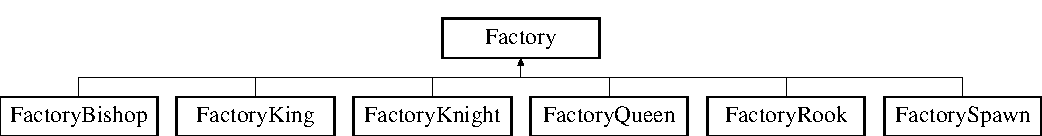
\includegraphics[height=1.830065cm]{class_factory}
\end{center}
\end{figure}
\subsection*{Fonctions membres publiques}
\begin{DoxyCompactItemize}
\item 
\hyperlink{class_factory_ac792bf88cfb7b6804b479529da5308cc}{Factory} ()
\begin{DoxyCompactList}\small\item\em Constructeur de \hyperlink{class_factory}{Factory}. \end{DoxyCompactList}\item 
virtual \hyperlink{class_factory_a8f71456f48e4df402c778a44191ff40e}{$\sim$\-Factory} ()
\begin{DoxyCompactList}\small\item\em Destructeur de \hyperlink{class_factory}{Factory}. \end{DoxyCompactList}\item 
virtual std\-::vector$<$ \hyperlink{class_piece}{Piece} $\ast$ $>$ \hyperlink{class_factory_a90f20f663caa6e5a5370465d3014630f}{build\-Pieces} (bool color)
\begin{DoxyCompactList}\small\item\em Permet de retourner une liste de Pièce$\ast$. \end{DoxyCompactList}\end{DoxyCompactItemize}


\subsection{Documentation des constructeurs et destructeur}
\hypertarget{class_factory_ac792bf88cfb7b6804b479529da5308cc}{\index{Factory@{Factory}!Factory@{Factory}}
\index{Factory@{Factory}!Factory@{Factory}}
\subsubsection[{Factory}]{\setlength{\rightskip}{0pt plus 5cm}Factory\-::\-Factory (
\begin{DoxyParamCaption}
{}
\end{DoxyParamCaption}
)}}\label{class_factory_ac792bf88cfb7b6804b479529da5308cc}


Constructeur de \hyperlink{class_factory}{Factory}. 

\hypertarget{class_factory_a8f71456f48e4df402c778a44191ff40e}{\index{Factory@{Factory}!$\sim$\-Factory@{$\sim$\-Factory}}
\index{$\sim$\-Factory@{$\sim$\-Factory}!Factory@{Factory}}
\subsubsection[{$\sim$\-Factory}]{\setlength{\rightskip}{0pt plus 5cm}Factory\-::$\sim$\-Factory (
\begin{DoxyParamCaption}
{}
\end{DoxyParamCaption}
)\hspace{0.3cm}{\ttfamily [virtual]}}}\label{class_factory_a8f71456f48e4df402c778a44191ff40e}


Destructeur de \hyperlink{class_factory}{Factory}. 



\subsection{Documentation des fonctions membres}
\hypertarget{class_factory_a90f20f663caa6e5a5370465d3014630f}{\index{Factory@{Factory}!build\-Pieces@{build\-Pieces}}
\index{build\-Pieces@{build\-Pieces}!Factory@{Factory}}
\subsubsection[{build\-Pieces}]{\setlength{\rightskip}{0pt plus 5cm}std\-::vector$<$ {\bf Piece} $\ast$ $>$ Factory\-::build\-Pieces (
\begin{DoxyParamCaption}
\item[{bool}]{color}
\end{DoxyParamCaption}
)\hspace{0.3cm}{\ttfamily [virtual]}}}\label{class_factory_a90f20f663caa6e5a5370465d3014630f}


Permet de retourner une liste de Pièce$\ast$. 


\begin{DoxyParams}{Paramètres}
{\em bool} & color, false signifie que l'équipe est white \\
\hline
\end{DoxyParams}
\begin{DoxyReturn}{Renvoie}
une liste de Piece$\ast$ 
\end{DoxyReturn}


Réimplémentée dans \hyperlink{class_factory_king_a0d5fd0a7340ab7bb50fe63e119c3a3ef}{Factory\-King}, \hyperlink{class_factory_queen_ac256e556b525b35d39f58af62fd1f962}{Factory\-Queen}, \hyperlink{class_factory_bishop_a501a01fc371b26931d528ea0aa8b5c14}{Factory\-Bishop}, \hyperlink{class_factory_knight_a25af606063189d96698aae45b1bfc1b9}{Factory\-Knight}, \hyperlink{class_factory_rook_a50ff41cf552af801c123bf2b28120c68}{Factory\-Rook}, et \hyperlink{class_factory_spawn_acdae41c4747246f35de741b32b3f74ac}{Factory\-Spawn}.



La documentation de cette classe a été générée à partir des fichiers suivants \-:\begin{DoxyCompactItemize}
\item 
src/\hyperlink{_factory_8hpp}{Factory.\-hpp}\item 
src/\hyperlink{_factory_8cpp}{Factory.\-cpp}\end{DoxyCompactItemize}

\hypertarget{class_factory_bishop}{\section{Référence de la classe Factory\-Bishop}
\label{class_factory_bishop}\index{Factory\-Bishop@{Factory\-Bishop}}
}


Classe \hyperlink{class_factory_bishop}{Factory\-Bishop} héritant de \hyperlink{class_factory}{Factory}.  




{\ttfamily \#include $<$Factory.\-hpp$>$}

Graphe d'héritage de Factory\-Bishop\-:\begin{figure}[H]
\begin{center}
\leavevmode
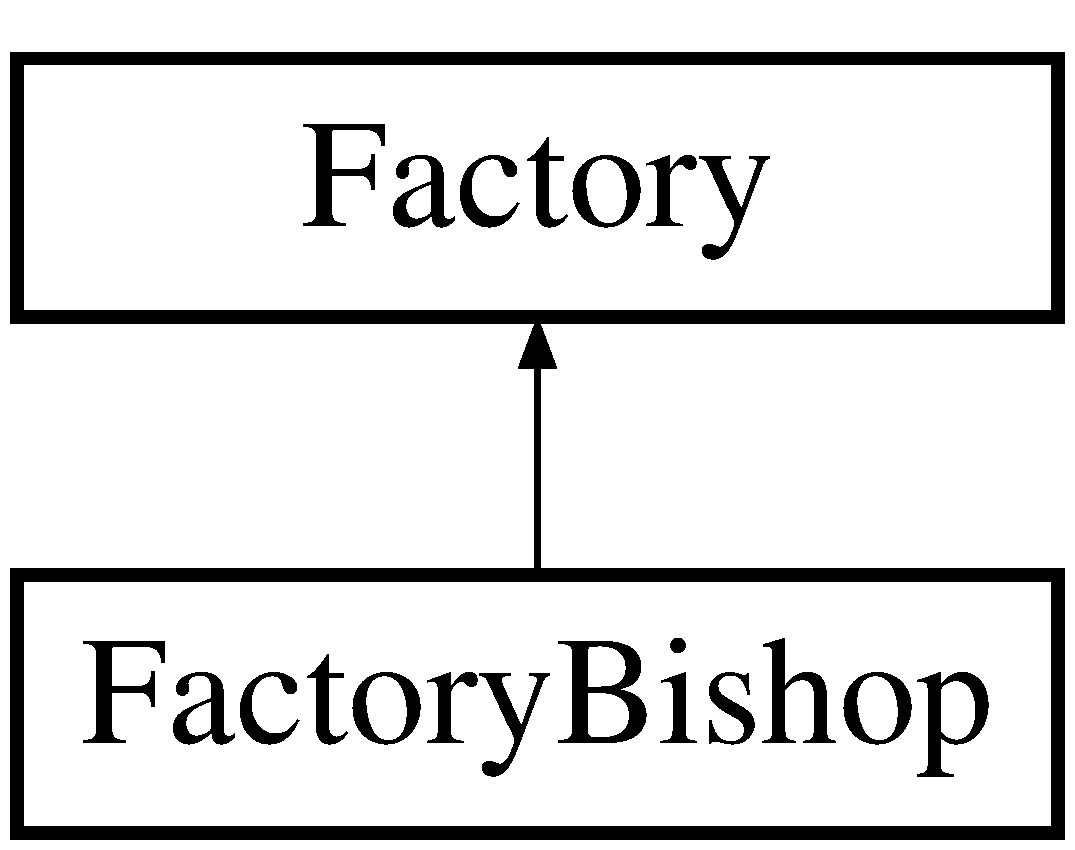
\includegraphics[height=2.000000cm]{class_factory_bishop}
\end{center}
\end{figure}
\subsection*{Fonctions membres publiques}
\begin{DoxyCompactItemize}
\item 
\hyperlink{class_factory_bishop_a6452991e628ec8262c57318da26171f1}{Factory\-Bishop} ()
\item 
\hyperlink{class_factory_bishop_aacec6859e5c70571357c5d172a62a38e}{$\sim$\-Factory\-Bishop} ()
\item 
std\-::vector$<$ \hyperlink{class_piece}{Piece} $\ast$ $>$ \hyperlink{class_factory_bishop_a501a01fc371b26931d528ea0aa8b5c14}{build\-Pieces} (bool color)
\end{DoxyCompactItemize}


\subsection{Description détaillée}
Classe \hyperlink{class_factory_bishop}{Factory\-Bishop} héritant de \hyperlink{class_factory}{Factory}. 

\subsection{Documentation des constructeurs et destructeur}
\hypertarget{class_factory_bishop_a6452991e628ec8262c57318da26171f1}{\index{Factory\-Bishop@{Factory\-Bishop}!Factory\-Bishop@{Factory\-Bishop}}
\index{Factory\-Bishop@{Factory\-Bishop}!FactoryBishop@{Factory\-Bishop}}
\subsubsection[{Factory\-Bishop}]{\setlength{\rightskip}{0pt plus 5cm}Factory\-Bishop\-::\-Factory\-Bishop (
\begin{DoxyParamCaption}
{}
\end{DoxyParamCaption}
)}}\label{class_factory_bishop_a6452991e628ec8262c57318da26171f1}
\hypertarget{class_factory_bishop_aacec6859e5c70571357c5d172a62a38e}{\index{Factory\-Bishop@{Factory\-Bishop}!$\sim$\-Factory\-Bishop@{$\sim$\-Factory\-Bishop}}
\index{$\sim$\-Factory\-Bishop@{$\sim$\-Factory\-Bishop}!FactoryBishop@{Factory\-Bishop}}
\subsubsection[{$\sim$\-Factory\-Bishop}]{\setlength{\rightskip}{0pt plus 5cm}Factory\-Bishop\-::$\sim$\-Factory\-Bishop (
\begin{DoxyParamCaption}
{}
\end{DoxyParamCaption}
)}}\label{class_factory_bishop_aacec6859e5c70571357c5d172a62a38e}


\subsection{Documentation des fonctions membres}
\hypertarget{class_factory_bishop_a501a01fc371b26931d528ea0aa8b5c14}{\index{Factory\-Bishop@{Factory\-Bishop}!build\-Pieces@{build\-Pieces}}
\index{build\-Pieces@{build\-Pieces}!FactoryBishop@{Factory\-Bishop}}
\subsubsection[{build\-Pieces}]{\setlength{\rightskip}{0pt plus 5cm}std\-::vector$<$ {\bf Piece} $\ast$ $>$ Factory\-Bishop\-::build\-Pieces (
\begin{DoxyParamCaption}
\item[{bool}]{color}
\end{DoxyParamCaption}
)\hspace{0.3cm}{\ttfamily [virtual]}}}\label{class_factory_bishop_a501a01fc371b26931d528ea0aa8b5c14}


Réimplémentée à partir de \hyperlink{class_factory_a90f20f663caa6e5a5370465d3014630f}{Factory}.



La documentation de cette classe a été générée à partir des fichiers suivants \-:\begin{DoxyCompactItemize}
\item 
src/\hyperlink{_factory_8hpp}{Factory.\-hpp}\item 
src/\hyperlink{_factory_8cpp}{Factory.\-cpp}\end{DoxyCompactItemize}

\hypertarget{class_factory_king}{\section{Référence de la classe Factory\-King}
\label{class_factory_king}\index{Factory\-King@{Factory\-King}}
}


Classe \hyperlink{class_factory_king}{Factory\-King} héritant de \hyperlink{class_factory}{Factory}.  




{\ttfamily \#include $<$Factory.\-hpp$>$}

Graphe d'héritage de Factory\-King\-:\begin{figure}[H]
\begin{center}
\leavevmode
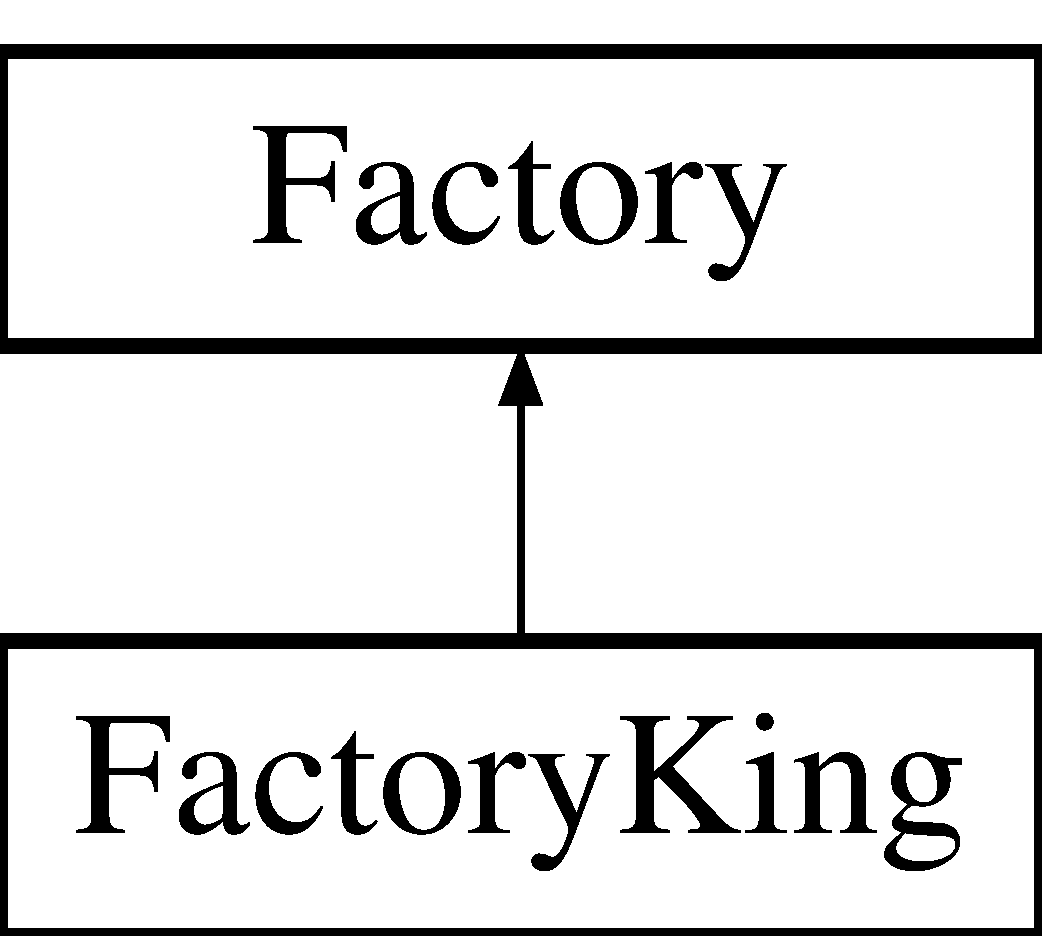
\includegraphics[height=2.000000cm]{class_factory_king}
\end{center}
\end{figure}
\subsection*{Fonctions membres publiques}
\begin{DoxyCompactItemize}
\item 
\hyperlink{class_factory_king_ad6762ceddcc10d41b5652e17455d3503}{Factory\-King} ()
\item 
\hyperlink{class_factory_king_adbf2005c439f045fb97bdb86147181a7}{$\sim$\-Factory\-King} ()
\item 
std\-::vector$<$ \hyperlink{class_piece}{Piece} $\ast$ $>$ \hyperlink{class_factory_king_a0d5fd0a7340ab7bb50fe63e119c3a3ef}{build\-Pieces} (bool color)
\end{DoxyCompactItemize}


\subsection{Description détaillée}
Classe \hyperlink{class_factory_king}{Factory\-King} héritant de \hyperlink{class_factory}{Factory}. 

\subsection{Documentation des constructeurs et destructeur}
\hypertarget{class_factory_king_ad6762ceddcc10d41b5652e17455d3503}{\index{Factory\-King@{Factory\-King}!Factory\-King@{Factory\-King}}
\index{Factory\-King@{Factory\-King}!FactoryKing@{Factory\-King}}
\subsubsection[{Factory\-King}]{\setlength{\rightskip}{0pt plus 5cm}Factory\-King\-::\-Factory\-King (
\begin{DoxyParamCaption}
{}
\end{DoxyParamCaption}
)}}\label{class_factory_king_ad6762ceddcc10d41b5652e17455d3503}
\hypertarget{class_factory_king_adbf2005c439f045fb97bdb86147181a7}{\index{Factory\-King@{Factory\-King}!$\sim$\-Factory\-King@{$\sim$\-Factory\-King}}
\index{$\sim$\-Factory\-King@{$\sim$\-Factory\-King}!FactoryKing@{Factory\-King}}
\subsubsection[{$\sim$\-Factory\-King}]{\setlength{\rightskip}{0pt plus 5cm}Factory\-King\-::$\sim$\-Factory\-King (
\begin{DoxyParamCaption}
{}
\end{DoxyParamCaption}
)}}\label{class_factory_king_adbf2005c439f045fb97bdb86147181a7}


\subsection{Documentation des fonctions membres}
\hypertarget{class_factory_king_a0d5fd0a7340ab7bb50fe63e119c3a3ef}{\index{Factory\-King@{Factory\-King}!build\-Pieces@{build\-Pieces}}
\index{build\-Pieces@{build\-Pieces}!FactoryKing@{Factory\-King}}
\subsubsection[{build\-Pieces}]{\setlength{\rightskip}{0pt plus 5cm}std\-::vector$<$ {\bf Piece} $\ast$ $>$ Factory\-King\-::build\-Pieces (
\begin{DoxyParamCaption}
\item[{bool}]{color}
\end{DoxyParamCaption}
)\hspace{0.3cm}{\ttfamily [virtual]}}}\label{class_factory_king_a0d5fd0a7340ab7bb50fe63e119c3a3ef}


Réimplémentée à partir de \hyperlink{class_factory_a90f20f663caa6e5a5370465d3014630f}{Factory}.



La documentation de cette classe a été générée à partir des fichiers suivants \-:\begin{DoxyCompactItemize}
\item 
src/\hyperlink{_factory_8hpp}{Factory.\-hpp}\item 
src/\hyperlink{_factory_8cpp}{Factory.\-cpp}\end{DoxyCompactItemize}

\hypertarget{class_factory_knight}{\section{Référence de la classe Factory\-Knight}
\label{class_factory_knight}\index{Factory\-Knight@{Factory\-Knight}}
}


Classe \hyperlink{class_factory_knight}{Factory\-Knight} héritant de \hyperlink{class_factory}{Factory}.  




{\ttfamily \#include $<$Factory.\-hpp$>$}

Graphe d'héritage de Factory\-Knight\-:\begin{figure}[H]
\begin{center}
\leavevmode
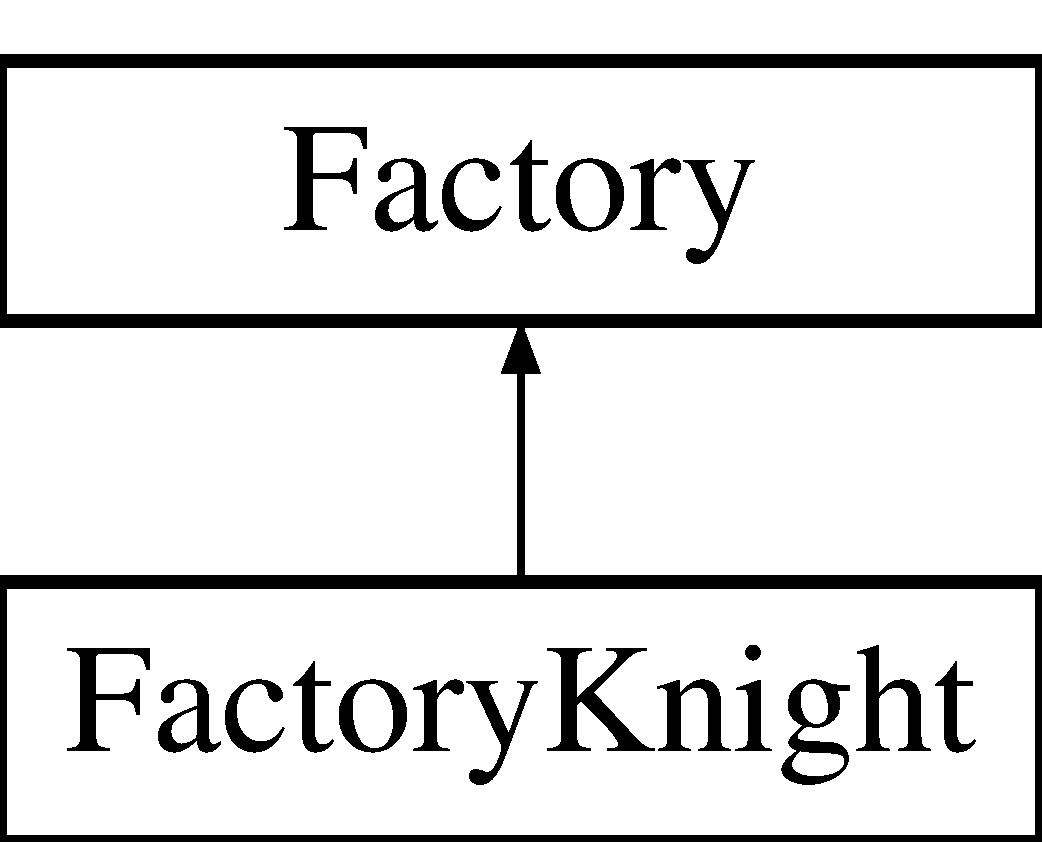
\includegraphics[height=2.000000cm]{class_factory_knight}
\end{center}
\end{figure}
\subsection*{Fonctions membres publiques}
\begin{DoxyCompactItemize}
\item 
\hyperlink{class_factory_knight_a4c3de6c385f4b3d02286e39cdbf99136}{Factory\-Knight} ()
\item 
\hyperlink{class_factory_knight_a40846bdf0be3fb8ecbcb50df3c4a7f61}{$\sim$\-Factory\-Knight} ()
\item 
std\-::vector$<$ \hyperlink{class_piece}{Piece} $\ast$ $>$ \hyperlink{class_factory_knight_a25af606063189d96698aae45b1bfc1b9}{build\-Pieces} (bool color)
\end{DoxyCompactItemize}


\subsection{Description détaillée}
Classe \hyperlink{class_factory_knight}{Factory\-Knight} héritant de \hyperlink{class_factory}{Factory}. 

\subsection{Documentation des constructeurs et destructeur}
\hypertarget{class_factory_knight_a4c3de6c385f4b3d02286e39cdbf99136}{\index{Factory\-Knight@{Factory\-Knight}!Factory\-Knight@{Factory\-Knight}}
\index{Factory\-Knight@{Factory\-Knight}!FactoryKnight@{Factory\-Knight}}
\subsubsection[{Factory\-Knight}]{\setlength{\rightskip}{0pt plus 5cm}Factory\-Knight\-::\-Factory\-Knight (
\begin{DoxyParamCaption}
{}
\end{DoxyParamCaption}
)}}\label{class_factory_knight_a4c3de6c385f4b3d02286e39cdbf99136}
\hypertarget{class_factory_knight_a40846bdf0be3fb8ecbcb50df3c4a7f61}{\index{Factory\-Knight@{Factory\-Knight}!$\sim$\-Factory\-Knight@{$\sim$\-Factory\-Knight}}
\index{$\sim$\-Factory\-Knight@{$\sim$\-Factory\-Knight}!FactoryKnight@{Factory\-Knight}}
\subsubsection[{$\sim$\-Factory\-Knight}]{\setlength{\rightskip}{0pt plus 5cm}Factory\-Knight\-::$\sim$\-Factory\-Knight (
\begin{DoxyParamCaption}
{}
\end{DoxyParamCaption}
)}}\label{class_factory_knight_a40846bdf0be3fb8ecbcb50df3c4a7f61}


\subsection{Documentation des fonctions membres}
\hypertarget{class_factory_knight_a25af606063189d96698aae45b1bfc1b9}{\index{Factory\-Knight@{Factory\-Knight}!build\-Pieces@{build\-Pieces}}
\index{build\-Pieces@{build\-Pieces}!FactoryKnight@{Factory\-Knight}}
\subsubsection[{build\-Pieces}]{\setlength{\rightskip}{0pt plus 5cm}std\-::vector$<$ {\bf Piece} $\ast$ $>$ Factory\-Knight\-::build\-Pieces (
\begin{DoxyParamCaption}
\item[{bool}]{color}
\end{DoxyParamCaption}
)\hspace{0.3cm}{\ttfamily [virtual]}}}\label{class_factory_knight_a25af606063189d96698aae45b1bfc1b9}


Réimplémentée à partir de \hyperlink{class_factory_a90f20f663caa6e5a5370465d3014630f}{Factory}.



La documentation de cette classe a été générée à partir des fichiers suivants \-:\begin{DoxyCompactItemize}
\item 
src/\hyperlink{_factory_8hpp}{Factory.\-hpp}\item 
src/\hyperlink{_factory_8cpp}{Factory.\-cpp}\end{DoxyCompactItemize}

\hypertarget{class_factory_queen}{\section{Référence de la classe Factory\-Queen}
\label{class_factory_queen}\index{Factory\-Queen@{Factory\-Queen}}
}


Classe \hyperlink{class_factory_queen}{Factory\-Queen} héritant de \hyperlink{class_factory}{Factory}.  




{\ttfamily \#include $<$Factory.\-hpp$>$}

Graphe d'héritage de Factory\-Queen\-:\begin{figure}[H]
\begin{center}
\leavevmode
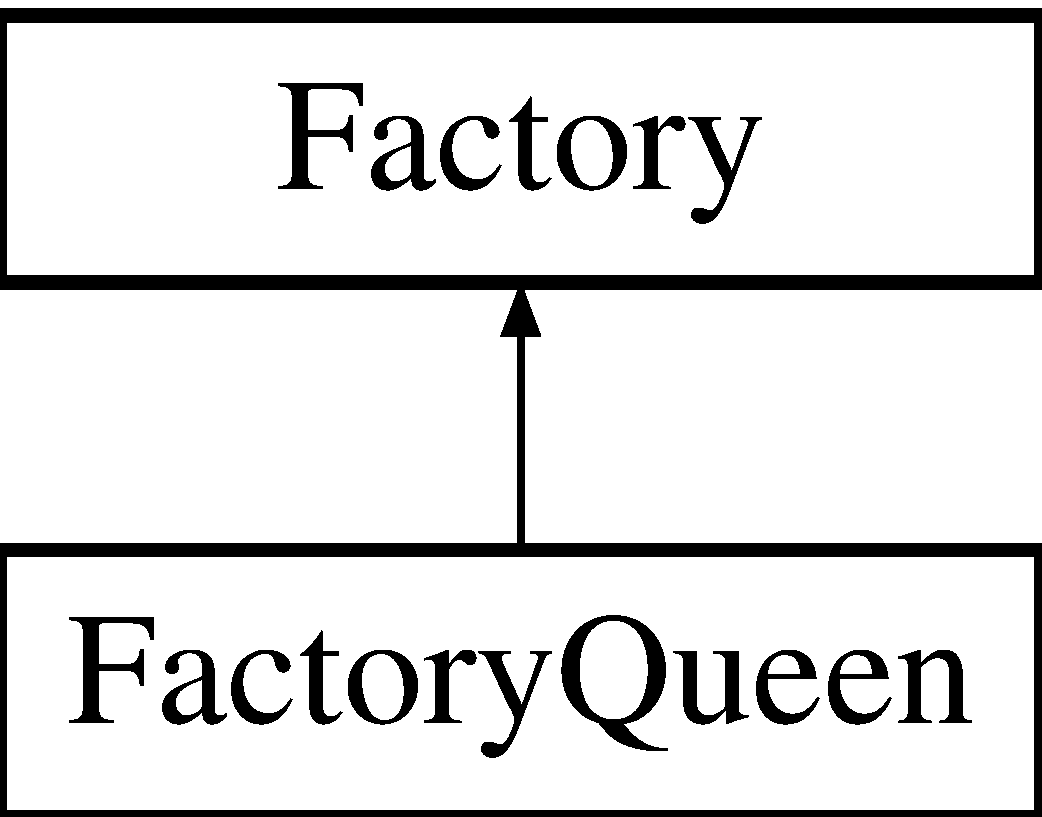
\includegraphics[height=2.000000cm]{class_factory_queen}
\end{center}
\end{figure}
\subsection*{Fonctions membres publiques}
\begin{DoxyCompactItemize}
\item 
\hyperlink{class_factory_queen_ab6cc7393c4cb1670ba041a44276a58cd}{Factory\-Queen} ()
\begin{DoxyCompactList}\small\item\em Constructeur de \hyperlink{class_factory_queen}{Factory\-Queen}. \end{DoxyCompactList}\item 
\hyperlink{class_factory_queen_ab1e9dfe91a868c88b775d3220b8f9bc0}{$\sim$\-Factory\-Queen} ()
\begin{DoxyCompactList}\small\item\em Destructeur de \hyperlink{class_factory_queen}{Factory\-Queen}. \end{DoxyCompactList}\item 
std\-::vector$<$ \hyperlink{class_piece}{Piece} $\ast$ $>$ \hyperlink{class_factory_queen_ac256e556b525b35d39f58af62fd1f962}{build\-Pieces} (bool color)
\begin{DoxyCompactList}\small\item\em Permet de retourner une liste de Pièce$\ast$ bien initialisée pour la reine normale. \end{DoxyCompactList}\end{DoxyCompactItemize}


\subsection{Description détaillée}
Classe \hyperlink{class_factory_queen}{Factory\-Queen} héritant de \hyperlink{class_factory}{Factory}. 

\subsection{Documentation des constructeurs et destructeur}
\hypertarget{class_factory_queen_ab6cc7393c4cb1670ba041a44276a58cd}{\index{Factory\-Queen@{Factory\-Queen}!Factory\-Queen@{Factory\-Queen}}
\index{Factory\-Queen@{Factory\-Queen}!FactoryQueen@{Factory\-Queen}}
\subsubsection[{Factory\-Queen}]{\setlength{\rightskip}{0pt plus 5cm}Factory\-Queen\-::\-Factory\-Queen (
\begin{DoxyParamCaption}
{}
\end{DoxyParamCaption}
)}}\label{class_factory_queen_ab6cc7393c4cb1670ba041a44276a58cd}


Constructeur de \hyperlink{class_factory_queen}{Factory\-Queen}. 

\hypertarget{class_factory_queen_ab1e9dfe91a868c88b775d3220b8f9bc0}{\index{Factory\-Queen@{Factory\-Queen}!$\sim$\-Factory\-Queen@{$\sim$\-Factory\-Queen}}
\index{$\sim$\-Factory\-Queen@{$\sim$\-Factory\-Queen}!FactoryQueen@{Factory\-Queen}}
\subsubsection[{$\sim$\-Factory\-Queen}]{\setlength{\rightskip}{0pt plus 5cm}Factory\-Queen\-::$\sim$\-Factory\-Queen (
\begin{DoxyParamCaption}
{}
\end{DoxyParamCaption}
)}}\label{class_factory_queen_ab1e9dfe91a868c88b775d3220b8f9bc0}


Destructeur de \hyperlink{class_factory_queen}{Factory\-Queen}. 



\subsection{Documentation des fonctions membres}
\hypertarget{class_factory_queen_ac256e556b525b35d39f58af62fd1f962}{\index{Factory\-Queen@{Factory\-Queen}!build\-Pieces@{build\-Pieces}}
\index{build\-Pieces@{build\-Pieces}!FactoryQueen@{Factory\-Queen}}
\subsubsection[{build\-Pieces}]{\setlength{\rightskip}{0pt plus 5cm}std\-::vector$<$ {\bf Piece} $\ast$ $>$ Factory\-Queen\-::build\-Pieces (
\begin{DoxyParamCaption}
\item[{bool}]{color}
\end{DoxyParamCaption}
)\hspace{0.3cm}{\ttfamily [virtual]}}}\label{class_factory_queen_ac256e556b525b35d39f58af62fd1f962}


Permet de retourner une liste de Pièce$\ast$ bien initialisée pour la reine normale. 


\begin{DoxyParams}{Paramètres}
{\em bool} & color, false signifie que l'équipe est white \\
\hline
\end{DoxyParams}
\begin{DoxyReturn}{Renvoie}
une liste de Piece$\ast$ 
\end{DoxyReturn}


Réimplémentée à partir de \hyperlink{class_factory_a90f20f663caa6e5a5370465d3014630f}{Factory}.



La documentation de cette classe a été générée à partir des fichiers suivants \-:\begin{DoxyCompactItemize}
\item 
src/\hyperlink{_factory_8hpp}{Factory.\-hpp}\item 
src/\hyperlink{_factory_8cpp}{Factory.\-cpp}\end{DoxyCompactItemize}

\hypertarget{class_factory_rook}{\section{Référence de la classe Factory\-Rook}
\label{class_factory_rook}\index{Factory\-Rook@{Factory\-Rook}}
}


Classe \hyperlink{class_factory_rook}{Factory\-Rook} héritant de \hyperlink{class_factory}{Factory}.  




{\ttfamily \#include $<$Factory.\-hpp$>$}

Graphe d'héritage de Factory\-Rook\-:\begin{figure}[H]
\begin{center}
\leavevmode
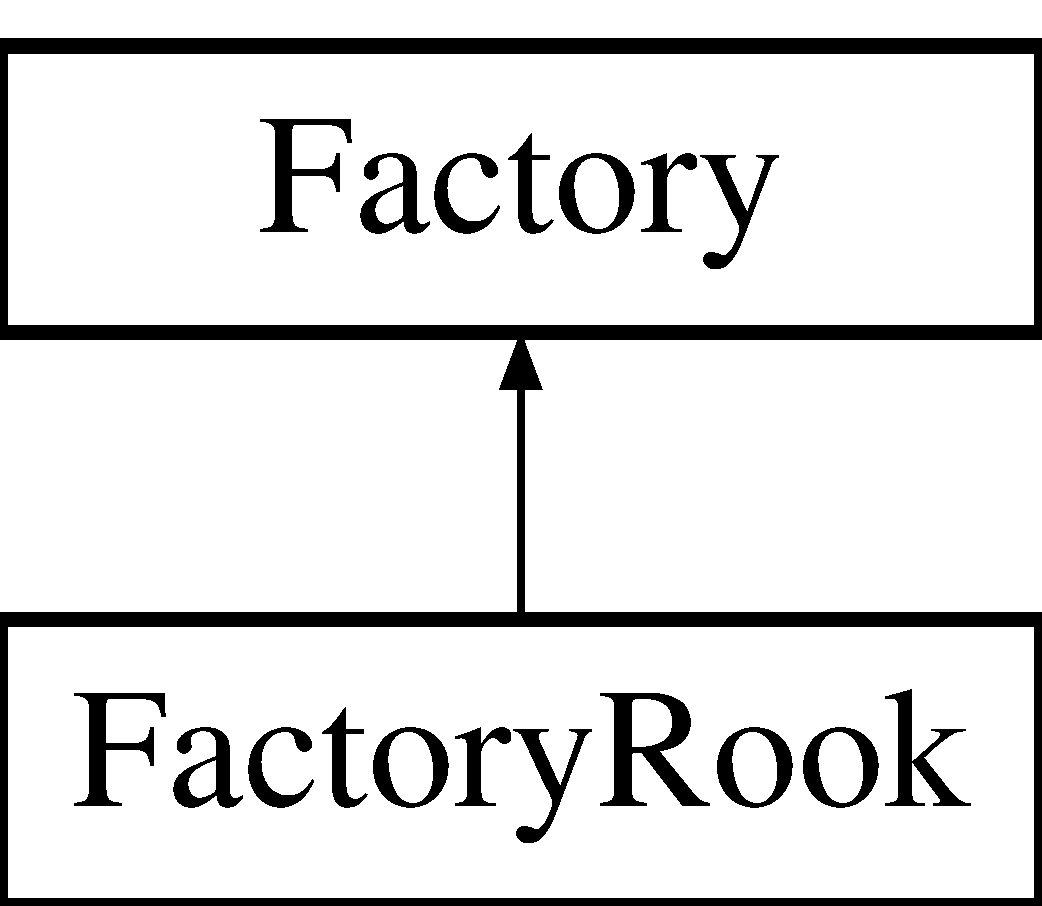
\includegraphics[height=2.000000cm]{class_factory_rook}
\end{center}
\end{figure}
\subsection*{Fonctions membres publiques}
\begin{DoxyCompactItemize}
\item 
\hyperlink{class_factory_rook_a4d8dfebcba093ee2f6009ffe907a8a8a}{Factory\-Rook} ()
\begin{DoxyCompactList}\small\item\em Constructeur de \hyperlink{class_factory_rook}{Factory\-Rook}. \end{DoxyCompactList}\item 
\hyperlink{class_factory_rook_a0bc1c85e0c4db96d877ccf00566470f4}{$\sim$\-Factory\-Rook} ()
\begin{DoxyCompactList}\small\item\em Destructeur de \hyperlink{class_factory_rook}{Factory\-Rook}. \end{DoxyCompactList}\item 
std\-::vector$<$ \hyperlink{class_piece}{Piece} $\ast$ $>$ \hyperlink{class_factory_rook_a50ff41cf552af801c123bf2b28120c68}{build\-Pieces} (bool color)
\begin{DoxyCompactList}\small\item\em Permet de retourner une liste de Pièce$\ast$ bien initialisée pour les Rooks normals. \end{DoxyCompactList}\end{DoxyCompactItemize}


\subsection{Description détaillée}
Classe \hyperlink{class_factory_rook}{Factory\-Rook} héritant de \hyperlink{class_factory}{Factory}. 

\subsection{Documentation des constructeurs et destructeur}
\hypertarget{class_factory_rook_a4d8dfebcba093ee2f6009ffe907a8a8a}{\index{Factory\-Rook@{Factory\-Rook}!Factory\-Rook@{Factory\-Rook}}
\index{Factory\-Rook@{Factory\-Rook}!FactoryRook@{Factory\-Rook}}
\subsubsection[{Factory\-Rook}]{\setlength{\rightskip}{0pt plus 5cm}Factory\-Rook\-::\-Factory\-Rook (
\begin{DoxyParamCaption}
{}
\end{DoxyParamCaption}
)}}\label{class_factory_rook_a4d8dfebcba093ee2f6009ffe907a8a8a}


Constructeur de \hyperlink{class_factory_rook}{Factory\-Rook}. 

\hypertarget{class_factory_rook_a0bc1c85e0c4db96d877ccf00566470f4}{\index{Factory\-Rook@{Factory\-Rook}!$\sim$\-Factory\-Rook@{$\sim$\-Factory\-Rook}}
\index{$\sim$\-Factory\-Rook@{$\sim$\-Factory\-Rook}!FactoryRook@{Factory\-Rook}}
\subsubsection[{$\sim$\-Factory\-Rook}]{\setlength{\rightskip}{0pt plus 5cm}Factory\-Rook\-::$\sim$\-Factory\-Rook (
\begin{DoxyParamCaption}
{}
\end{DoxyParamCaption}
)}}\label{class_factory_rook_a0bc1c85e0c4db96d877ccf00566470f4}


Destructeur de \hyperlink{class_factory_rook}{Factory\-Rook}. 



\subsection{Documentation des fonctions membres}
\hypertarget{class_factory_rook_a50ff41cf552af801c123bf2b28120c68}{\index{Factory\-Rook@{Factory\-Rook}!build\-Pieces@{build\-Pieces}}
\index{build\-Pieces@{build\-Pieces}!FactoryRook@{Factory\-Rook}}
\subsubsection[{build\-Pieces}]{\setlength{\rightskip}{0pt plus 5cm}std\-::vector$<$ {\bf Piece} $\ast$ $>$ Factory\-Rook\-::build\-Pieces (
\begin{DoxyParamCaption}
\item[{bool}]{color}
\end{DoxyParamCaption}
)\hspace{0.3cm}{\ttfamily [virtual]}}}\label{class_factory_rook_a50ff41cf552af801c123bf2b28120c68}


Permet de retourner une liste de Pièce$\ast$ bien initialisée pour les Rooks normals. 


\begin{DoxyParams}{Paramètres}
{\em bool} & color, false signifie que l'équipe est white \\
\hline
\end{DoxyParams}
\begin{DoxyReturn}{Renvoie}
une liste de Piece$\ast$ 
\end{DoxyReturn}


Réimplémentée à partir de \hyperlink{class_factory_a90f20f663caa6e5a5370465d3014630f}{Factory}.



La documentation de cette classe a été générée à partir des fichiers suivants \-:\begin{DoxyCompactItemize}
\item 
src/\hyperlink{_factory_8hpp}{Factory.\-hpp}\item 
src/\hyperlink{_factory_8cpp}{Factory.\-cpp}\end{DoxyCompactItemize}

\hypertarget{class_factory_spawn}{\section{Référence de la classe Factory\-Spawn}
\label{class_factory_spawn}\index{Factory\-Spawn@{Factory\-Spawn}}
}


Classe \hyperlink{class_factory_spawn}{Factory\-Spawn} héritant de \hyperlink{class_factory}{Factory}.  




{\ttfamily \#include $<$Factory.\-hpp$>$}

Graphe d'héritage de Factory\-Spawn\-:\begin{figure}[H]
\begin{center}
\leavevmode
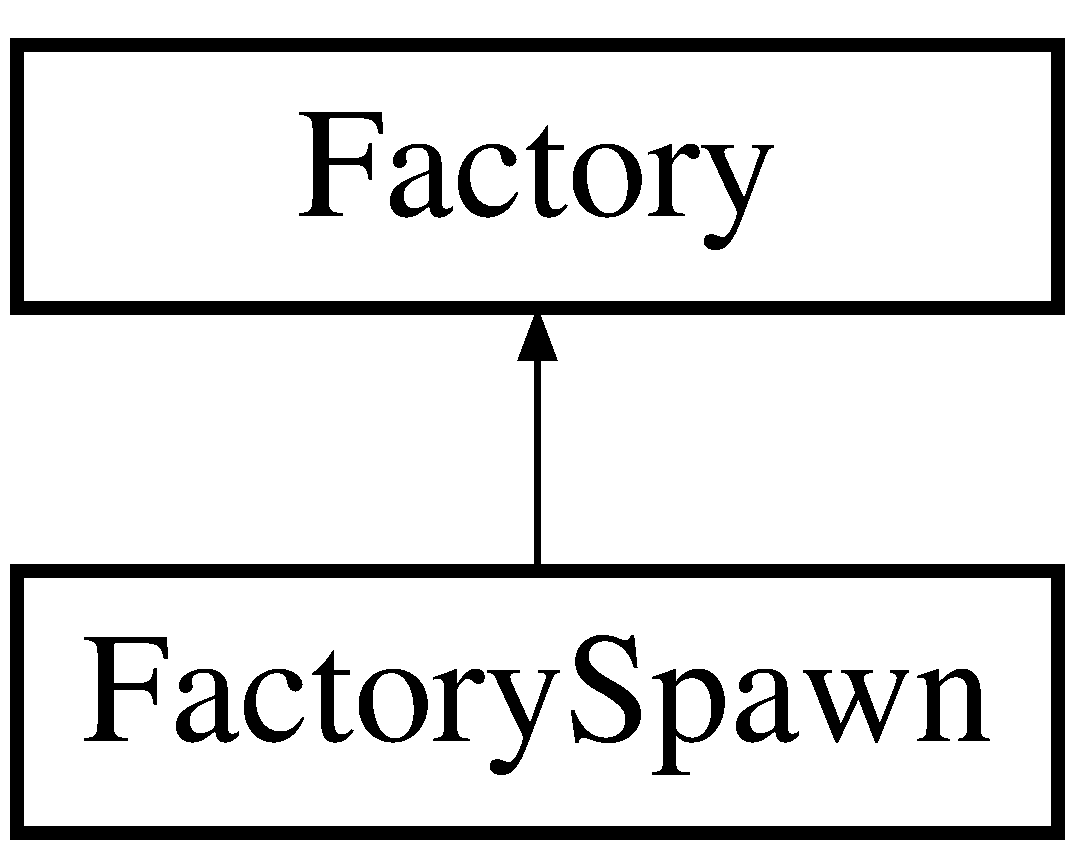
\includegraphics[height=2.000000cm]{class_factory_spawn}
\end{center}
\end{figure}
\subsection*{Fonctions membres publiques}
\begin{DoxyCompactItemize}
\item 
\hyperlink{class_factory_spawn_afa2ea203f016dc06217ab48607c4e899}{Factory\-Spawn} ()
\begin{DoxyCompactList}\small\item\em Constructeur de \hyperlink{class_factory_spawn}{Factory\-Spawn}. \end{DoxyCompactList}\item 
\hyperlink{class_factory_spawn_ae7ec52abd4b3dc1e49cd9988a1d1d9bc}{$\sim$\-Factory\-Spawn} ()
\begin{DoxyCompactList}\small\item\em Destructeur de \hyperlink{class_factory_spawn}{Factory\-Spawn}. \end{DoxyCompactList}\item 
std\-::vector$<$ \hyperlink{class_piece}{Piece} $\ast$ $>$ \hyperlink{class_factory_spawn_acdae41c4747246f35de741b32b3f74ac}{build\-Pieces} (bool color)
\begin{DoxyCompactList}\small\item\em Permet de retourner une liste de Pièce$\ast$ bien initialisée pour les spawns normals. \end{DoxyCompactList}\end{DoxyCompactItemize}


\subsection{Description détaillée}
Classe \hyperlink{class_factory_spawn}{Factory\-Spawn} héritant de \hyperlink{class_factory}{Factory}. 

\subsection{Documentation des constructeurs et destructeur}
\hypertarget{class_factory_spawn_afa2ea203f016dc06217ab48607c4e899}{\index{Factory\-Spawn@{Factory\-Spawn}!Factory\-Spawn@{Factory\-Spawn}}
\index{Factory\-Spawn@{Factory\-Spawn}!FactorySpawn@{Factory\-Spawn}}
\subsubsection[{Factory\-Spawn}]{\setlength{\rightskip}{0pt plus 5cm}Factory\-Spawn\-::\-Factory\-Spawn (
\begin{DoxyParamCaption}
{}
\end{DoxyParamCaption}
)}}\label{class_factory_spawn_afa2ea203f016dc06217ab48607c4e899}


Constructeur de \hyperlink{class_factory_spawn}{Factory\-Spawn}. 

\hypertarget{class_factory_spawn_ae7ec52abd4b3dc1e49cd9988a1d1d9bc}{\index{Factory\-Spawn@{Factory\-Spawn}!$\sim$\-Factory\-Spawn@{$\sim$\-Factory\-Spawn}}
\index{$\sim$\-Factory\-Spawn@{$\sim$\-Factory\-Spawn}!FactorySpawn@{Factory\-Spawn}}
\subsubsection[{$\sim$\-Factory\-Spawn}]{\setlength{\rightskip}{0pt plus 5cm}Factory\-Spawn\-::$\sim$\-Factory\-Spawn (
\begin{DoxyParamCaption}
{}
\end{DoxyParamCaption}
)}}\label{class_factory_spawn_ae7ec52abd4b3dc1e49cd9988a1d1d9bc}


Destructeur de \hyperlink{class_factory_spawn}{Factory\-Spawn}. 



\subsection{Documentation des fonctions membres}
\hypertarget{class_factory_spawn_acdae41c4747246f35de741b32b3f74ac}{\index{Factory\-Spawn@{Factory\-Spawn}!build\-Pieces@{build\-Pieces}}
\index{build\-Pieces@{build\-Pieces}!FactorySpawn@{Factory\-Spawn}}
\subsubsection[{build\-Pieces}]{\setlength{\rightskip}{0pt plus 5cm}std\-::vector$<$ {\bf Piece} $\ast$ $>$ Factory\-Spawn\-::build\-Pieces (
\begin{DoxyParamCaption}
\item[{bool}]{color}
\end{DoxyParamCaption}
)\hspace{0.3cm}{\ttfamily [virtual]}}}\label{class_factory_spawn_acdae41c4747246f35de741b32b3f74ac}


Permet de retourner une liste de Pièce$\ast$ bien initialisée pour les spawns normals. 


\begin{DoxyParams}{Paramètres}
{\em bool} & color, false signifie que l'équipe est white \\
\hline
\end{DoxyParams}
\begin{DoxyReturn}{Renvoie}
une liste de Piece$\ast$ 
\end{DoxyReturn}


Réimplémentée à partir de \hyperlink{class_factory_a90f20f663caa6e5a5370465d3014630f}{Factory}.



La documentation de cette classe a été générée à partir des fichiers suivants \-:\begin{DoxyCompactItemize}
\item 
src/\hyperlink{_factory_8hpp}{Factory.\-hpp}\item 
src/\hyperlink{_factory_8cpp}{Factory.\-cpp}\end{DoxyCompactItemize}

\hypertarget{class_game_state}{\section{Référence de la classe Game\-State}
\label{class_game_state}\index{Game\-State@{Game\-State}}
}


{\ttfamily \#include $<$State.\-hpp$>$}

Graphe d'héritage de Game\-State\-:\begin{figure}[H]
\begin{center}
\leavevmode
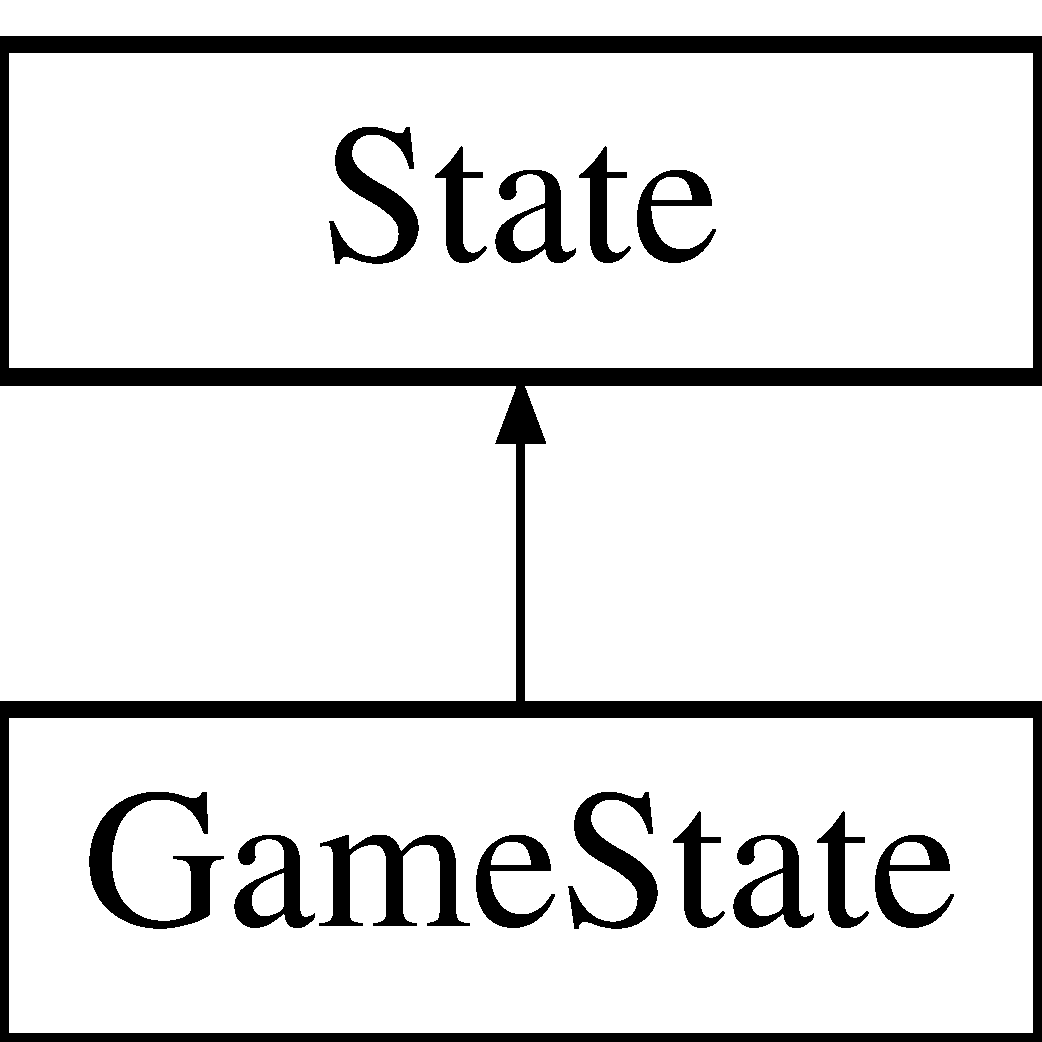
\includegraphics[height=2.000000cm]{class_game_state}
\end{center}
\end{figure}
\subsection*{Fonctions membres publiques}
\begin{DoxyCompactItemize}
\item 
\hyperlink{class_game_state_a564f9ae19ac9980b28b78944645b5163}{Game\-State} (\hyperlink{class_player}{Player} $\ast$p)
\begin{DoxyCompactList}\small\item\em Constructeur, crée un Etat\-Jeu à l'aide du constructeur de \hyperlink{class_state}{State} avec un Joueur en paramètre. \end{DoxyCompactList}\item 
\hyperlink{class_game_state_ae623df5042cd0c17daa3394fdcb397b3}{$\sim$\-Game\-State} ()
\begin{DoxyCompactList}\small\item\em Destructeur de l'objet \hyperlink{class_game_state}{Game\-State}. \end{DoxyCompactList}\item 
void \hyperlink{class_game_state_af0290fd87a2bc2a44119dc700d8b8721}{in\-Game} ()
\begin{DoxyCompactList}\small\item\em Définition de la procédure virtuelle, pas d'effet dans cet Etat là \end{DoxyCompactList}\item 
void \hyperlink{class_game_state_a646e5436c4191f323dfa736a06e79695}{check} ()
\begin{DoxyCompactList}\small\item\em Définition de la procédure virtuelle, transition vers l'état \hyperlink{class_check_state}{Check\-State}. \end{DoxyCompactList}\item 
void \hyperlink{class_game_state_ada8cd91a048922c4d8aedbef17ce6fbc}{check\-Mate} ()
\begin{DoxyCompactList}\small\item\em Définition de la procédure virtuelle, transition vers l'état \hyperlink{class_mate_state}{Mate\-State}. \end{DoxyCompactList}\item 
void \hyperlink{class_game_state_a006f729bc30cfa224d3235c87e5a6e59}{game\-Null} ()
\begin{DoxyCompactList}\small\item\em Définition de la procédure virtuelle, transition vers l'état \hyperlink{class_null_state}{Null\-State}. \end{DoxyCompactList}\item 
void \hyperlink{class_game_state_a65fc1ef481baa95f675ff8a78aa14e05}{game\-End} ()
\begin{DoxyCompactList}\small\item\em Définition de la procédure virtuelle, pas d'effet dans cet Etat là \end{DoxyCompactList}\item 
void \hyperlink{class_game_state_a9ccc5473c6f04e60711cb9a438b276e5}{print} ()
\begin{DoxyCompactList}\small\item\em Définition de la procédure virtuelle, affiche l'état \hyperlink{class_game_state}{Game\-State}. \end{DoxyCompactList}\item 
bool \hyperlink{class_game_state_ae0f8b04f85ed4dfbbd4c2a6a06827273}{ischeck} ()
\begin{DoxyCompactList}\small\item\em procédure virtuelle permettant de savoir s'il se trouve en position d'echec \end{DoxyCompactList}\item 
bool \hyperlink{class_game_state_ac9b5e18d5bec890d741cc0eae4bb5600}{is\-Check\-Mate} ()
\begin{DoxyCompactList}\small\item\em procédure virtuelle permettant de savoir s'il se trouve en position d'echec et mate \end{DoxyCompactList}\item 
bool \hyperlink{class_game_state_a777e982cbef6125ba4003f68d6292825}{isnulle} ()
\begin{DoxyCompactList}\small\item\em procédure virtuelle permettant de savoir s'il se trouve en position nulle \end{DoxyCompactList}\end{DoxyCompactItemize}
\subsection*{Membres hérités additionnels}


\subsection{Documentation des constructeurs et destructeur}
\hypertarget{class_game_state_a564f9ae19ac9980b28b78944645b5163}{\index{Game\-State@{Game\-State}!Game\-State@{Game\-State}}
\index{Game\-State@{Game\-State}!GameState@{Game\-State}}
\subsubsection[{Game\-State}]{\setlength{\rightskip}{0pt plus 5cm}Game\-State\-::\-Game\-State (
\begin{DoxyParamCaption}
\item[{{\bf Player} $\ast$}]{p}
\end{DoxyParamCaption}
)}}\label{class_game_state_a564f9ae19ac9980b28b78944645b5163}


Constructeur, crée un Etat\-Jeu à l'aide du constructeur de \hyperlink{class_state}{State} avec un Joueur en paramètre. 


\begin{DoxyParams}{Paramètres}
{\em p} & \\
\hline
\end{DoxyParams}
\hypertarget{class_game_state_ae623df5042cd0c17daa3394fdcb397b3}{\index{Game\-State@{Game\-State}!$\sim$\-Game\-State@{$\sim$\-Game\-State}}
\index{$\sim$\-Game\-State@{$\sim$\-Game\-State}!GameState@{Game\-State}}
\subsubsection[{$\sim$\-Game\-State}]{\setlength{\rightskip}{0pt plus 5cm}Game\-State\-::$\sim$\-Game\-State (
\begin{DoxyParamCaption}
{}
\end{DoxyParamCaption}
)}}\label{class_game_state_ae623df5042cd0c17daa3394fdcb397b3}


Destructeur de l'objet \hyperlink{class_game_state}{Game\-State}. 



\subsection{Documentation des fonctions membres}
\hypertarget{class_game_state_a646e5436c4191f323dfa736a06e79695}{\index{Game\-State@{Game\-State}!check@{check}}
\index{check@{check}!GameState@{Game\-State}}
\subsubsection[{check}]{\setlength{\rightskip}{0pt plus 5cm}void Game\-State\-::check (
\begin{DoxyParamCaption}
{}
\end{DoxyParamCaption}
)\hspace{0.3cm}{\ttfamily [virtual]}}}\label{class_game_state_a646e5436c4191f323dfa736a06e79695}


Définition de la procédure virtuelle, transition vers l'état \hyperlink{class_check_state}{Check\-State}. 



Implémente \hyperlink{class_state_a321fd726bbefc35fedbbf001d2a37021}{State}.

\hypertarget{class_game_state_ada8cd91a048922c4d8aedbef17ce6fbc}{\index{Game\-State@{Game\-State}!check\-Mate@{check\-Mate}}
\index{check\-Mate@{check\-Mate}!GameState@{Game\-State}}
\subsubsection[{check\-Mate}]{\setlength{\rightskip}{0pt plus 5cm}void Game\-State\-::check\-Mate (
\begin{DoxyParamCaption}
{}
\end{DoxyParamCaption}
)\hspace{0.3cm}{\ttfamily [virtual]}}}\label{class_game_state_ada8cd91a048922c4d8aedbef17ce6fbc}


Définition de la procédure virtuelle, transition vers l'état \hyperlink{class_mate_state}{Mate\-State}. 



Implémente \hyperlink{class_state_aa2b89ec92ecd4f6271269fe4b8ccc790}{State}.

\hypertarget{class_game_state_a65fc1ef481baa95f675ff8a78aa14e05}{\index{Game\-State@{Game\-State}!game\-End@{game\-End}}
\index{game\-End@{game\-End}!GameState@{Game\-State}}
\subsubsection[{game\-End}]{\setlength{\rightskip}{0pt plus 5cm}void Game\-State\-::game\-End (
\begin{DoxyParamCaption}
{}
\end{DoxyParamCaption}
)\hspace{0.3cm}{\ttfamily [virtual]}}}\label{class_game_state_a65fc1ef481baa95f675ff8a78aa14e05}


Définition de la procédure virtuelle, pas d'effet dans cet Etat là 



Implémente \hyperlink{class_state_a5117e1f9bf06e17b4b0277838fe39bd8}{State}.

\hypertarget{class_game_state_a006f729bc30cfa224d3235c87e5a6e59}{\index{Game\-State@{Game\-State}!game\-Null@{game\-Null}}
\index{game\-Null@{game\-Null}!GameState@{Game\-State}}
\subsubsection[{game\-Null}]{\setlength{\rightskip}{0pt plus 5cm}void Game\-State\-::game\-Null (
\begin{DoxyParamCaption}
{}
\end{DoxyParamCaption}
)\hspace{0.3cm}{\ttfamily [virtual]}}}\label{class_game_state_a006f729bc30cfa224d3235c87e5a6e59}


Définition de la procédure virtuelle, transition vers l'état \hyperlink{class_null_state}{Null\-State}. 



Implémente \hyperlink{class_state_ad5b7fe10b2c30243f36d7d0950c50d43}{State}.

\hypertarget{class_game_state_af0290fd87a2bc2a44119dc700d8b8721}{\index{Game\-State@{Game\-State}!in\-Game@{in\-Game}}
\index{in\-Game@{in\-Game}!GameState@{Game\-State}}
\subsubsection[{in\-Game}]{\setlength{\rightskip}{0pt plus 5cm}void Game\-State\-::in\-Game (
\begin{DoxyParamCaption}
{}
\end{DoxyParamCaption}
)\hspace{0.3cm}{\ttfamily [virtual]}}}\label{class_game_state_af0290fd87a2bc2a44119dc700d8b8721}


Définition de la procédure virtuelle, pas d'effet dans cet Etat là 



Implémente \hyperlink{class_state_a738b04d6e0c12a39bf96a2a7159202d8}{State}.

\hypertarget{class_game_state_ae0f8b04f85ed4dfbbd4c2a6a06827273}{\index{Game\-State@{Game\-State}!ischeck@{ischeck}}
\index{ischeck@{ischeck}!GameState@{Game\-State}}
\subsubsection[{ischeck}]{\setlength{\rightskip}{0pt plus 5cm}bool Game\-State\-::ischeck (
\begin{DoxyParamCaption}
{}
\end{DoxyParamCaption}
)\hspace{0.3cm}{\ttfamily [virtual]}}}\label{class_game_state_ae0f8b04f85ed4dfbbd4c2a6a06827273}


procédure virtuelle permettant de savoir s'il se trouve en position d'echec 



Implémente \hyperlink{class_state_ad2d7084c507d8d20be2e772d953129fb}{State}.

\hypertarget{class_game_state_ac9b5e18d5bec890d741cc0eae4bb5600}{\index{Game\-State@{Game\-State}!is\-Check\-Mate@{is\-Check\-Mate}}
\index{is\-Check\-Mate@{is\-Check\-Mate}!GameState@{Game\-State}}
\subsubsection[{is\-Check\-Mate}]{\setlength{\rightskip}{0pt plus 5cm}bool Game\-State\-::is\-Check\-Mate (
\begin{DoxyParamCaption}
{}
\end{DoxyParamCaption}
)\hspace{0.3cm}{\ttfamily [virtual]}}}\label{class_game_state_ac9b5e18d5bec890d741cc0eae4bb5600}


procédure virtuelle permettant de savoir s'il se trouve en position d'echec et mate 



Implémente \hyperlink{class_state_ac67ccfcdc2d3e9fbe6d05961416ffeda}{State}.

\hypertarget{class_game_state_a777e982cbef6125ba4003f68d6292825}{\index{Game\-State@{Game\-State}!isnulle@{isnulle}}
\index{isnulle@{isnulle}!GameState@{Game\-State}}
\subsubsection[{isnulle}]{\setlength{\rightskip}{0pt plus 5cm}bool Game\-State\-::isnulle (
\begin{DoxyParamCaption}
{}
\end{DoxyParamCaption}
)\hspace{0.3cm}{\ttfamily [virtual]}}}\label{class_game_state_a777e982cbef6125ba4003f68d6292825}


procédure virtuelle permettant de savoir s'il se trouve en position nulle 



Implémente \hyperlink{class_state_a869f2ebfad7e60719df5f89a613adee1}{State}.

\hypertarget{class_game_state_a9ccc5473c6f04e60711cb9a438b276e5}{\index{Game\-State@{Game\-State}!print@{print}}
\index{print@{print}!GameState@{Game\-State}}
\subsubsection[{print}]{\setlength{\rightskip}{0pt plus 5cm}void Game\-State\-::print (
\begin{DoxyParamCaption}
{}
\end{DoxyParamCaption}
)\hspace{0.3cm}{\ttfamily [virtual]}}}\label{class_game_state_a9ccc5473c6f04e60711cb9a438b276e5}


Définition de la procédure virtuelle, affiche l'état \hyperlink{class_game_state}{Game\-State}. 



Implémente \hyperlink{class_state_a95a537bb55b9118b23d5bed88ba3b335}{State}.



La documentation de cette classe a été générée à partir des fichiers suivants \-:\begin{DoxyCompactItemize}
\item 
src/\hyperlink{_state_8hpp}{State.\-hpp}\item 
src/\hyperlink{_state_8cpp}{State.\-cpp}\end{DoxyCompactItemize}

\hypertarget{class_king}{\section{Référence de la classe King}
\label{class_king}\index{King@{King}}
}


Classe \hyperlink{class_king}{King} héritant de \hyperlink{class_piece}{Piece}.  




{\ttfamily \#include $<$Piece.\-hpp$>$}

Graphe d'héritage de King\-:\begin{figure}[H]
\begin{center}
\leavevmode
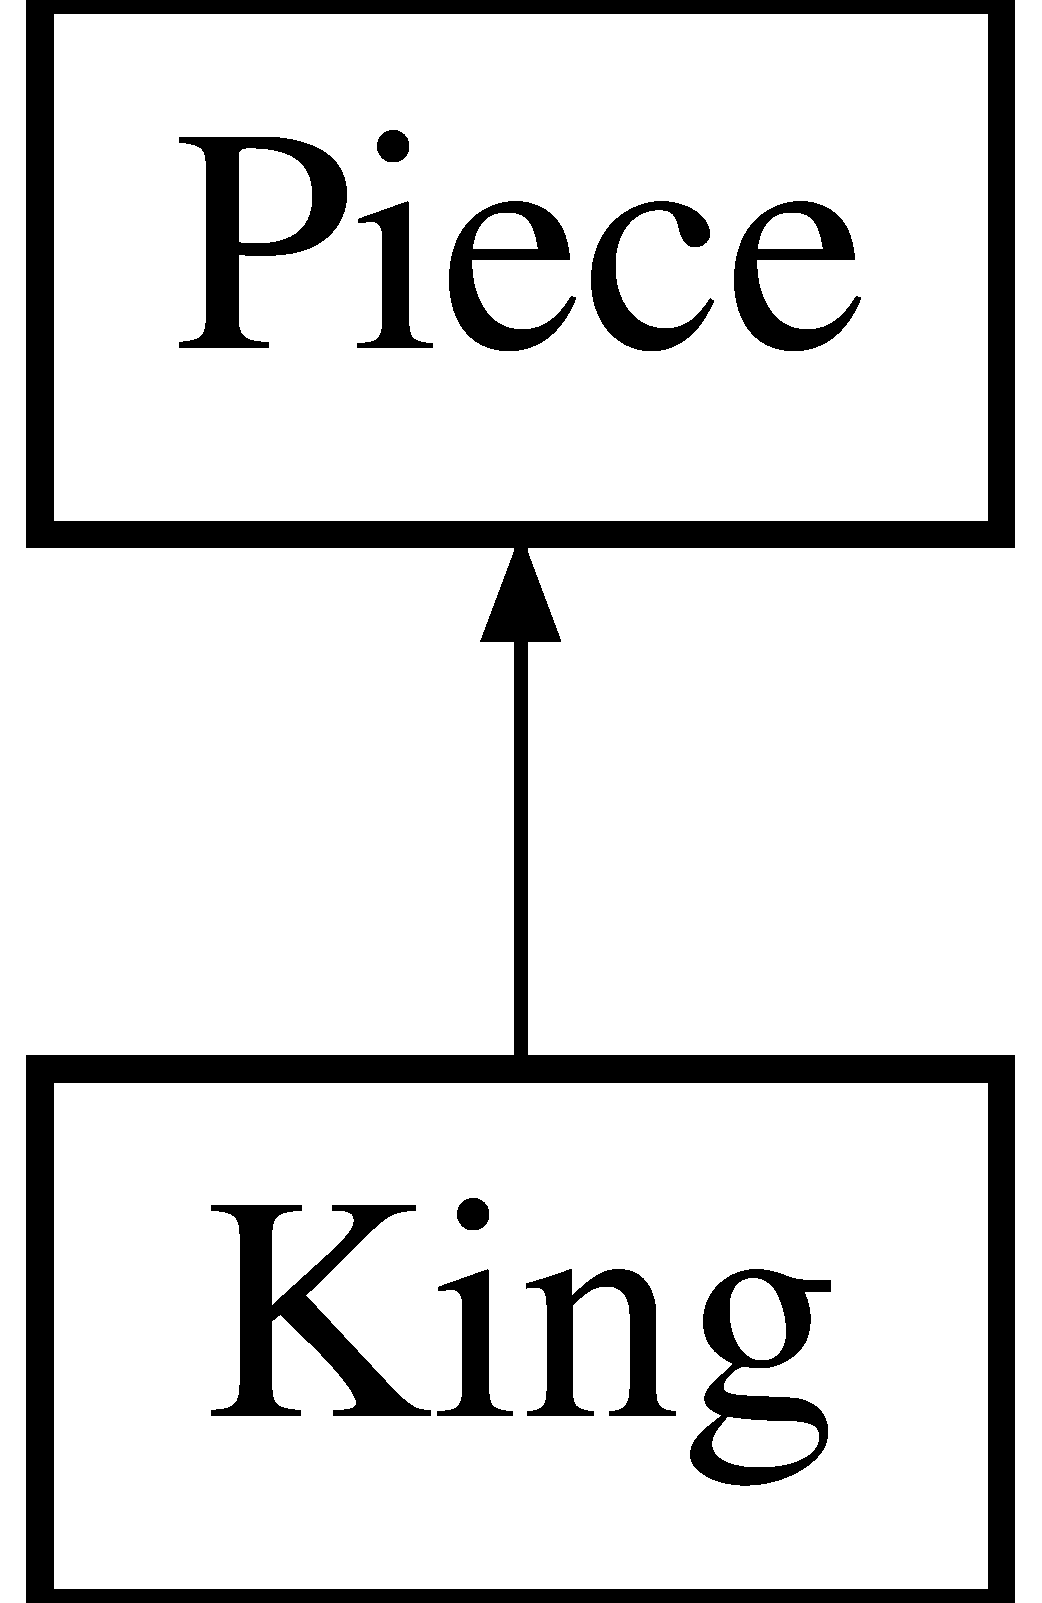
\includegraphics[height=2.000000cm]{class_king}
\end{center}
\end{figure}
\subsection*{Fonctions membres publiques}
\begin{DoxyCompactItemize}
\item 
\hyperlink{class_king_af934f2cda4bb5baca66c2ae114997b6e}{King} (unsigned int x, unsigned int y)
\begin{DoxyCompactList}\small\item\em Constructeur, crée un objet \hyperlink{class_king}{King} d'une couleur mise en paramètre. \end{DoxyCompactList}\item 
\hyperlink{class_king_aac368ce96e2b12f62e3608d27262e941}{$\sim$\-King} ()
\begin{DoxyCompactList}\small\item\em Destructeur d'un objet \hyperlink{class_king}{King}. \end{DoxyCompactList}\item 
bool \hyperlink{class_king_a1e7d9da6599c3e3ab9cbc4d5026f0dcf}{as\-Moved} ()
\begin{DoxyCompactList}\small\item\em Getter de l'attribut \-\_\-moved. \end{DoxyCompactList}\item 
void \hyperlink{class_king_a29a4ff10443abb0b0ecd088c88861d18}{set\-Moved} (bool new\-Moved)
\begin{DoxyCompactList}\small\item\em Setter de l'attribut \-\_\-moved. \end{DoxyCompactList}\item 
virtual void \hyperlink{class_king_aabc0b7a9a553383e7aba11daecbbc61c}{movement} ()
\begin{DoxyCompactList}\small\item\em procédure virtuelle permettant de mettre à jour l'attribut movements en fonction des déplacements possibles du Roi \end{DoxyCompactList}\end{DoxyCompactItemize}
\subsection*{Membres hérités additionnels}


\subsection{Description détaillée}
Classe \hyperlink{class_king}{King} héritant de \hyperlink{class_piece}{Piece}. 

\subsection{Documentation des constructeurs et destructeur}
\hypertarget{class_king_af934f2cda4bb5baca66c2ae114997b6e}{\index{King@{King}!King@{King}}
\index{King@{King}!King@{King}}
\subsubsection[{King}]{\setlength{\rightskip}{0pt plus 5cm}King\-::\-King (
\begin{DoxyParamCaption}
\item[{unsigned int}]{x, }
\item[{unsigned int}]{y}
\end{DoxyParamCaption}
)}}\label{class_king_af934f2cda4bb5baca66c2ae114997b6e}


Constructeur, crée un objet \hyperlink{class_king}{King} d'une couleur mise en paramètre. 


\begin{DoxyParams}{Paramètres}
{\em string} & color \\
\hline
\end{DoxyParams}
\hypertarget{class_king_aac368ce96e2b12f62e3608d27262e941}{\index{King@{King}!$\sim$\-King@{$\sim$\-King}}
\index{$\sim$\-King@{$\sim$\-King}!King@{King}}
\subsubsection[{$\sim$\-King}]{\setlength{\rightskip}{0pt plus 5cm}King\-::$\sim$\-King (
\begin{DoxyParamCaption}
{}
\end{DoxyParamCaption}
)}}\label{class_king_aac368ce96e2b12f62e3608d27262e941}


Destructeur d'un objet \hyperlink{class_king}{King}. 



\subsection{Documentation des fonctions membres}
\hypertarget{class_king_a1e7d9da6599c3e3ab9cbc4d5026f0dcf}{\index{King@{King}!as\-Moved@{as\-Moved}}
\index{as\-Moved@{as\-Moved}!King@{King}}
\subsubsection[{as\-Moved}]{\setlength{\rightskip}{0pt plus 5cm}bool King\-::as\-Moved (
\begin{DoxyParamCaption}
{}
\end{DoxyParamCaption}
)}}\label{class_king_a1e7d9da6599c3e3ab9cbc4d5026f0dcf}


Getter de l'attribut \-\_\-moved. 

\begin{DoxyReturn}{Renvoie}
attribut \-\_\-moved 
\end{DoxyReturn}
\hypertarget{class_king_aabc0b7a9a553383e7aba11daecbbc61c}{\index{King@{King}!movement@{movement}}
\index{movement@{movement}!King@{King}}
\subsubsection[{movement}]{\setlength{\rightskip}{0pt plus 5cm}void King\-::movement (
\begin{DoxyParamCaption}
{}
\end{DoxyParamCaption}
)\hspace{0.3cm}{\ttfamily [virtual]}}}\label{class_king_aabc0b7a9a553383e7aba11daecbbc61c}


procédure virtuelle permettant de mettre à jour l'attribut movements en fonction des déplacements possibles du Roi 



Réimplémentée à partir de \hyperlink{class_piece_ae721b5ed94376fd4e7d348d36739ed4d}{Piece}.

\hypertarget{class_king_a29a4ff10443abb0b0ecd088c88861d18}{\index{King@{King}!set\-Moved@{set\-Moved}}
\index{set\-Moved@{set\-Moved}!King@{King}}
\subsubsection[{set\-Moved}]{\setlength{\rightskip}{0pt plus 5cm}void King\-::set\-Moved (
\begin{DoxyParamCaption}
\item[{bool}]{new\-Moved}
\end{DoxyParamCaption}
)}}\label{class_king_a29a4ff10443abb0b0ecd088c88861d18}


Setter de l'attribut \-\_\-moved. 


\begin{DoxyParams}{Paramètres}
{\em bool} & new\-Moved \\
\hline
\end{DoxyParams}


La documentation de cette classe a été générée à partir des fichiers suivants \-:\begin{DoxyCompactItemize}
\item 
src/\hyperlink{_piece_8hpp}{Piece.\-hpp}\item 
src/\hyperlink{_piece_8cpp}{Piece.\-cpp}\end{DoxyCompactItemize}

\hypertarget{class_knight}{\section{Référence de la classe Knight}
\label{class_knight}\index{Knight@{Knight}}
}


Classe \hyperlink{class_knight}{Knight} héritant de \hyperlink{class_piece}{Piece}.  




{\ttfamily \#include $<$Piece.\-hpp$>$}

Graphe d'héritage de Knight\-:\begin{figure}[H]
\begin{center}
\leavevmode
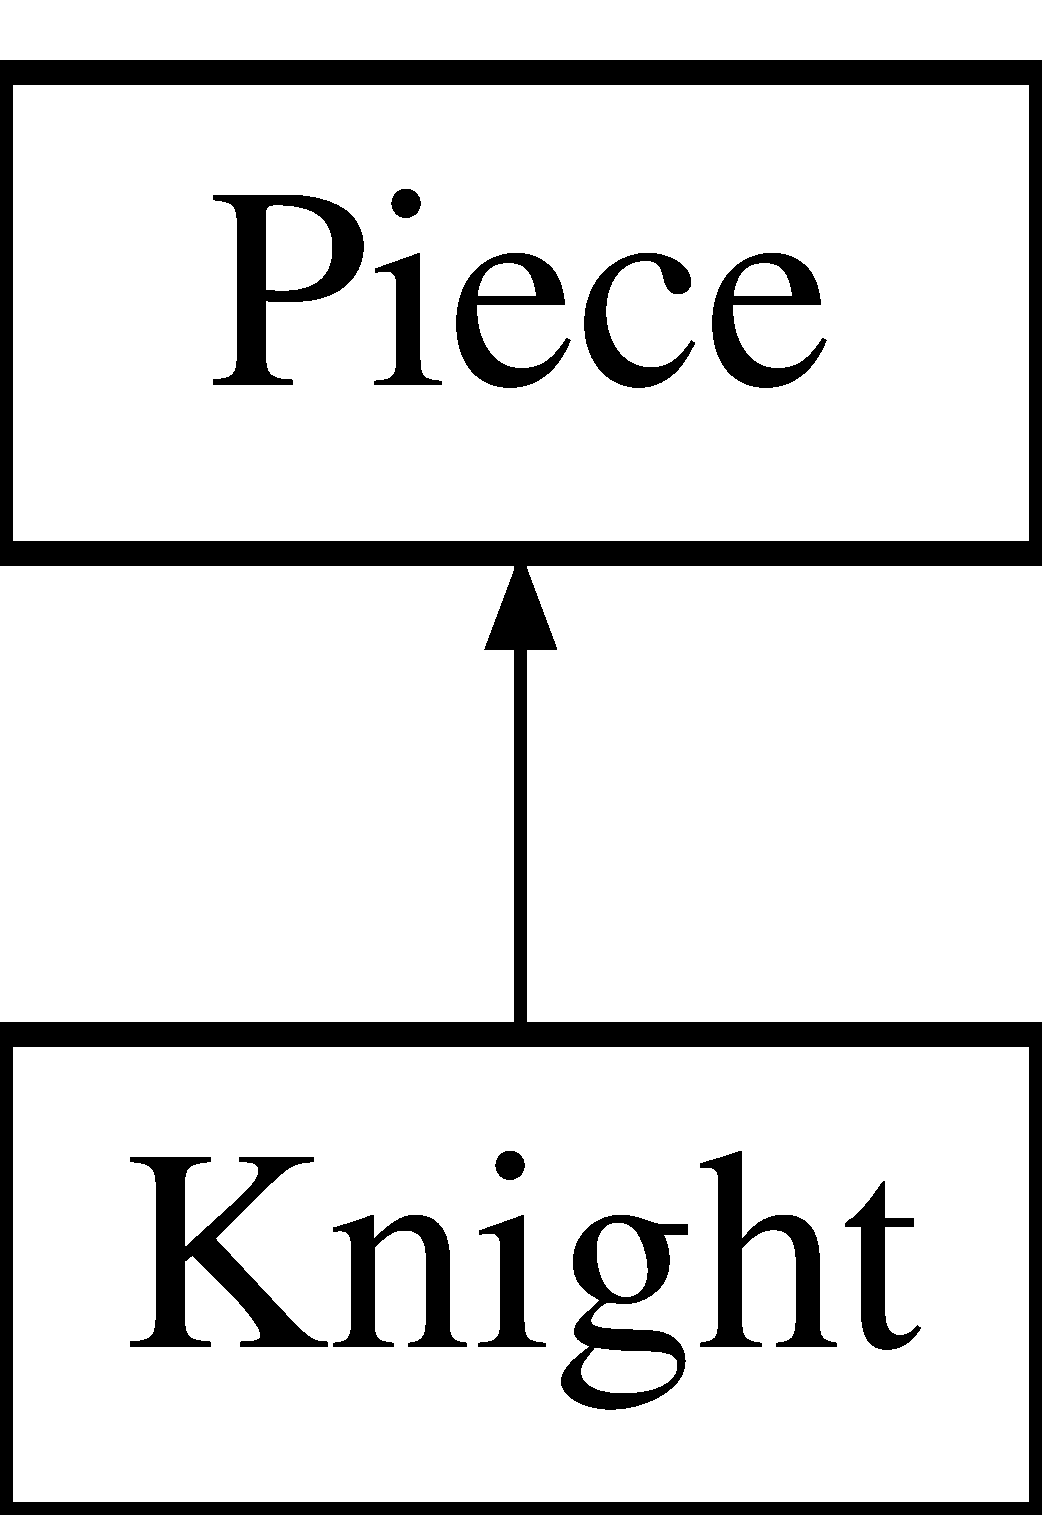
\includegraphics[height=2.000000cm]{class_knight}
\end{center}
\end{figure}
\subsection*{Fonctions membres publiques}
\begin{DoxyCompactItemize}
\item 
\hyperlink{class_knight_ae39d8e49ade7c0b66cf35dad69f2d2db}{Knight} (unsigned int x, unsigned int y)
\begin{DoxyCompactList}\small\item\em Constructeur, crée un objet \hyperlink{class_knight}{Knight} de coordonnées x,y. \end{DoxyCompactList}\item 
\hyperlink{class_knight_a2754123d6876babe915f4da8f761361b}{$\sim$\-Knight} ()
\begin{DoxyCompactList}\small\item\em Destructeur d'un objet cavalier. \end{DoxyCompactList}\item 
virtual void \hyperlink{class_knight_ab228b385a3154ecdc18fce4cc0df9cd6}{movement} ()
\begin{DoxyCompactList}\small\item\em procédure virtuelle permettant de mettre à jour l'attribut movements en fonction des déplacements possibles du Cavalier \end{DoxyCompactList}\end{DoxyCompactItemize}
\subsection*{Membres hérités additionnels}


\subsection{Description détaillée}
Classe \hyperlink{class_knight}{Knight} héritant de \hyperlink{class_piece}{Piece}. 

\subsection{Documentation des constructeurs et destructeur}
\hypertarget{class_knight_ae39d8e49ade7c0b66cf35dad69f2d2db}{\index{Knight@{Knight}!Knight@{Knight}}
\index{Knight@{Knight}!Knight@{Knight}}
\subsubsection[{Knight}]{\setlength{\rightskip}{0pt plus 5cm}Knight\-::\-Knight (
\begin{DoxyParamCaption}
\item[{unsigned int}]{x, }
\item[{unsigned int}]{y}
\end{DoxyParamCaption}
)}}\label{class_knight_ae39d8e49ade7c0b66cf35dad69f2d2db}


Constructeur, crée un objet \hyperlink{class_knight}{Knight} de coordonnées x,y. 


\begin{DoxyParams}{Paramètres}
{\em unsigned} & int x \\
\hline
{\em unsigned} & int y \\
\hline
\end{DoxyParams}
\hypertarget{class_knight_a2754123d6876babe915f4da8f761361b}{\index{Knight@{Knight}!$\sim$\-Knight@{$\sim$\-Knight}}
\index{$\sim$\-Knight@{$\sim$\-Knight}!Knight@{Knight}}
\subsubsection[{$\sim$\-Knight}]{\setlength{\rightskip}{0pt plus 5cm}Knight\-::$\sim$\-Knight (
\begin{DoxyParamCaption}
{}
\end{DoxyParamCaption}
)}}\label{class_knight_a2754123d6876babe915f4da8f761361b}


Destructeur d'un objet cavalier. 



\subsection{Documentation des fonctions membres}
\hypertarget{class_knight_ab228b385a3154ecdc18fce4cc0df9cd6}{\index{Knight@{Knight}!movement@{movement}}
\index{movement@{movement}!Knight@{Knight}}
\subsubsection[{movement}]{\setlength{\rightskip}{0pt plus 5cm}void Knight\-::movement (
\begin{DoxyParamCaption}
{}
\end{DoxyParamCaption}
)\hspace{0.3cm}{\ttfamily [virtual]}}}\label{class_knight_ab228b385a3154ecdc18fce4cc0df9cd6}


procédure virtuelle permettant de mettre à jour l'attribut movements en fonction des déplacements possibles du Cavalier 



Réimplémentée à partir de \hyperlink{class_piece_ae721b5ed94376fd4e7d348d36739ed4d}{Piece}.



La documentation de cette classe a été générée à partir des fichiers suivants \-:\begin{DoxyCompactItemize}
\item 
src/\hyperlink{_piece_8hpp}{Piece.\-hpp}\item 
src/\hyperlink{_piece_8cpp}{Piece.\-cpp}\end{DoxyCompactItemize}

\hypertarget{class_mate_state}{\section{Référence de la classe Mate\-State}
\label{class_mate_state}\index{Mate\-State@{Mate\-State}}
}


{\ttfamily \#include $<$State.\-hpp$>$}

Graphe d'héritage de Mate\-State\-:\begin{figure}[H]
\begin{center}
\leavevmode
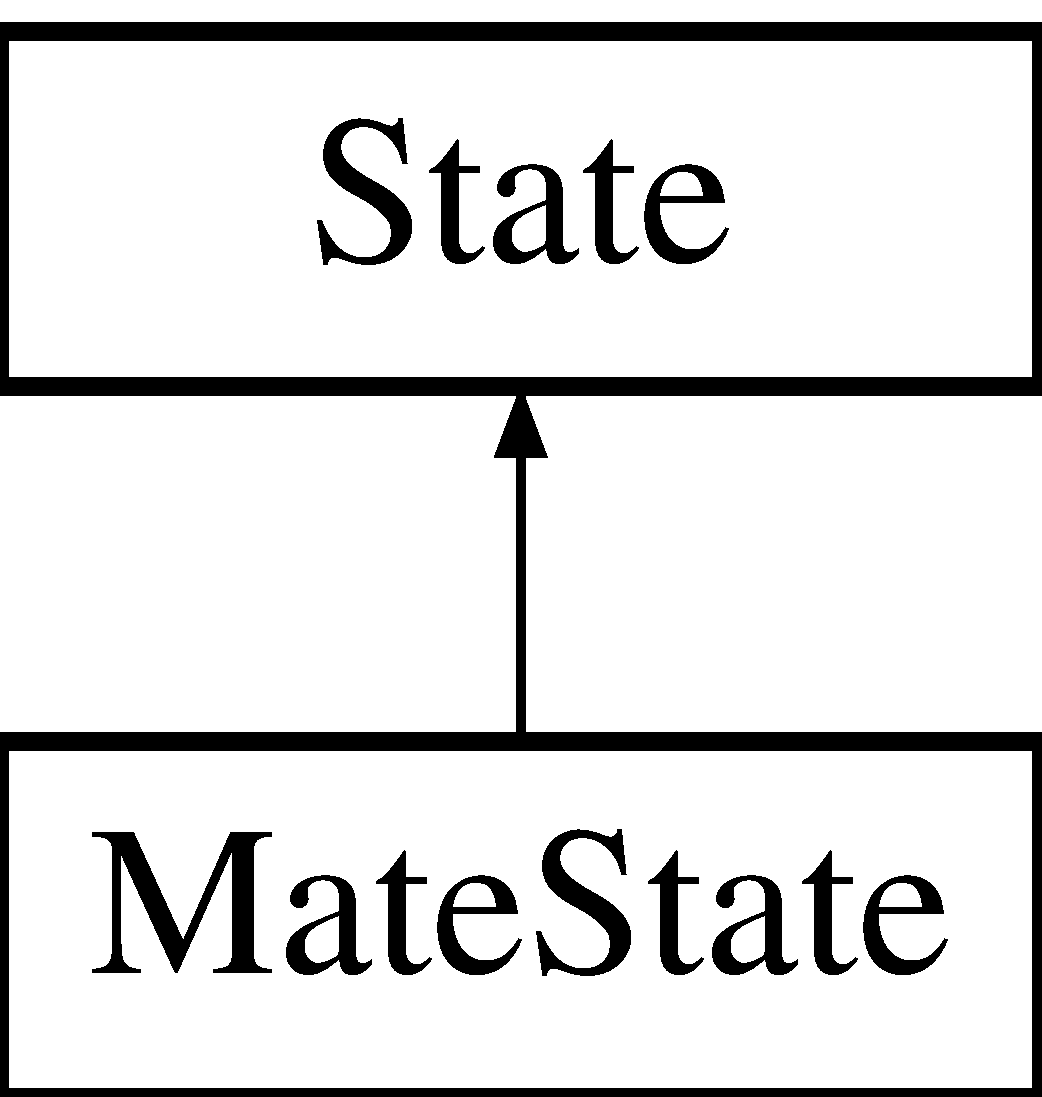
\includegraphics[height=2.000000cm]{class_mate_state}
\end{center}
\end{figure}
\subsection*{Fonctions membres publiques}
\begin{DoxyCompactItemize}
\item 
\hyperlink{class_mate_state_aa4a8a6d8614ffddaeac5cf19b2707136}{Mate\-State} (\hyperlink{class_player}{Player} $\ast$p)
\begin{DoxyCompactList}\small\item\em Constructeur, crée un Etat\-Mate à l'aide du constructeur de \hyperlink{class_state}{State} avec un Joueur en paramètre. \end{DoxyCompactList}\item 
\hyperlink{class_mate_state_af75f5df59f008abe5e1913e1d55acbad}{$\sim$\-Mate\-State} ()
\begin{DoxyCompactList}\small\item\em Destructeur de l'objet \hyperlink{class_mate_state}{Mate\-State}. \end{DoxyCompactList}\item 
void \hyperlink{class_mate_state_a99575ed4587f029511bc5bd1ec9ab262}{in\-Game} ()
\begin{DoxyCompactList}\small\item\em Définition de la procédure virtuelle, pas d'effet dans cet Etat là \end{DoxyCompactList}\item 
void \hyperlink{class_mate_state_a2205b5879c63fcdf469002d9d5203bb3}{check} ()
\begin{DoxyCompactList}\small\item\em Définition de la procédure virtuelle, pas d'effet dans cet Etat là \end{DoxyCompactList}\item 
void \hyperlink{class_mate_state_af785a3407109dd3d0a6868a358c92213}{check\-Mate} ()
\begin{DoxyCompactList}\small\item\em Définition de la procédure virtuelle, pas d'effet dans cet Etat là \end{DoxyCompactList}\item 
void \hyperlink{class_mate_state_a59ad17cb3366c560b921619d52f00181}{game\-Null} ()
\begin{DoxyCompactList}\small\item\em Définition de la procédure virtuelle, pas d'effet dans cet Etat là \end{DoxyCompactList}\item 
void \hyperlink{class_mate_state_a19b4fa2115a36da6e1dd333a617ee7bb}{game\-End} ()
\begin{DoxyCompactList}\small\item\em Définition de la procédure virtuelle, transition vers l'état End\-Game. \end{DoxyCompactList}\item 
void \hyperlink{class_mate_state_ab96d11c6cbb289483659d55bb8735c77}{print} ()
\begin{DoxyCompactList}\small\item\em Définition de la procédure virtuelle, affiche l'état \hyperlink{class_mate_state}{Mate\-State}. \end{DoxyCompactList}\item 
bool \hyperlink{class_mate_state_a9b9eb5923dc94adb69b28174d580c3b1}{ischeckmate} ()
\begin{DoxyCompactList}\small\item\em procédure virtuelle permettant de savoir s'il se trouve en possition d'echec \end{DoxyCompactList}\item 
bool \hyperlink{class_mate_state_a47e7642586f54efaa977755bb2b2311d}{ischeck} ()
\begin{DoxyCompactList}\small\item\em procédure virtuelle permettant de savoir s'il se trouve en possition d'echec et mate \end{DoxyCompactList}\item 
bool \hyperlink{class_mate_state_a0d586f9c4dafd94ebfa6b14e425fff8b}{isnulle} ()
\begin{DoxyCompactList}\small\item\em procédure virtuelle permettant de savoir s'il se trouve en possition nulle \end{DoxyCompactList}\end{DoxyCompactItemize}
\subsection*{Membres hérités additionnels}


\subsection{Documentation des constructeurs et destructeur}
\hypertarget{class_mate_state_aa4a8a6d8614ffddaeac5cf19b2707136}{\index{Mate\-State@{Mate\-State}!Mate\-State@{Mate\-State}}
\index{Mate\-State@{Mate\-State}!MateState@{Mate\-State}}
\subsubsection[{Mate\-State}]{\setlength{\rightskip}{0pt plus 5cm}Mate\-State\-::\-Mate\-State (
\begin{DoxyParamCaption}
\item[{{\bf Player} $\ast$}]{p}
\end{DoxyParamCaption}
)}}\label{class_mate_state_aa4a8a6d8614ffddaeac5cf19b2707136}


Constructeur, crée un Etat\-Mate à l'aide du constructeur de \hyperlink{class_state}{State} avec un Joueur en paramètre. 


\begin{DoxyParams}{Paramètres}
{\em p} & \\
\hline
\end{DoxyParams}
\hypertarget{class_mate_state_af75f5df59f008abe5e1913e1d55acbad}{\index{Mate\-State@{Mate\-State}!$\sim$\-Mate\-State@{$\sim$\-Mate\-State}}
\index{$\sim$\-Mate\-State@{$\sim$\-Mate\-State}!MateState@{Mate\-State}}
\subsubsection[{$\sim$\-Mate\-State}]{\setlength{\rightskip}{0pt plus 5cm}Mate\-State\-::$\sim$\-Mate\-State (
\begin{DoxyParamCaption}
{}
\end{DoxyParamCaption}
)}}\label{class_mate_state_af75f5df59f008abe5e1913e1d55acbad}


Destructeur de l'objet \hyperlink{class_mate_state}{Mate\-State}. 



\subsection{Documentation des fonctions membres}
\hypertarget{class_mate_state_a2205b5879c63fcdf469002d9d5203bb3}{\index{Mate\-State@{Mate\-State}!check@{check}}
\index{check@{check}!MateState@{Mate\-State}}
\subsubsection[{check}]{\setlength{\rightskip}{0pt plus 5cm}void Mate\-State\-::check (
\begin{DoxyParamCaption}
{}
\end{DoxyParamCaption}
)\hspace{0.3cm}{\ttfamily [virtual]}}}\label{class_mate_state_a2205b5879c63fcdf469002d9d5203bb3}


Définition de la procédure virtuelle, pas d'effet dans cet Etat là 



Implémente \hyperlink{class_state_a321fd726bbefc35fedbbf001d2a37021}{State}.

\hypertarget{class_mate_state_af785a3407109dd3d0a6868a358c92213}{\index{Mate\-State@{Mate\-State}!check\-Mate@{check\-Mate}}
\index{check\-Mate@{check\-Mate}!MateState@{Mate\-State}}
\subsubsection[{check\-Mate}]{\setlength{\rightskip}{0pt plus 5cm}void Mate\-State\-::check\-Mate (
\begin{DoxyParamCaption}
{}
\end{DoxyParamCaption}
)\hspace{0.3cm}{\ttfamily [virtual]}}}\label{class_mate_state_af785a3407109dd3d0a6868a358c92213}


Définition de la procédure virtuelle, pas d'effet dans cet Etat là 



Implémente \hyperlink{class_state_aa2b89ec92ecd4f6271269fe4b8ccc790}{State}.

\hypertarget{class_mate_state_a19b4fa2115a36da6e1dd333a617ee7bb}{\index{Mate\-State@{Mate\-State}!game\-End@{game\-End}}
\index{game\-End@{game\-End}!MateState@{Mate\-State}}
\subsubsection[{game\-End}]{\setlength{\rightskip}{0pt plus 5cm}void Mate\-State\-::game\-End (
\begin{DoxyParamCaption}
{}
\end{DoxyParamCaption}
)\hspace{0.3cm}{\ttfamily [virtual]}}}\label{class_mate_state_a19b4fa2115a36da6e1dd333a617ee7bb}


Définition de la procédure virtuelle, transition vers l'état End\-Game. 



Implémente \hyperlink{class_state_a5117e1f9bf06e17b4b0277838fe39bd8}{State}.

\hypertarget{class_mate_state_a59ad17cb3366c560b921619d52f00181}{\index{Mate\-State@{Mate\-State}!game\-Null@{game\-Null}}
\index{game\-Null@{game\-Null}!MateState@{Mate\-State}}
\subsubsection[{game\-Null}]{\setlength{\rightskip}{0pt plus 5cm}void Mate\-State\-::game\-Null (
\begin{DoxyParamCaption}
{}
\end{DoxyParamCaption}
)\hspace{0.3cm}{\ttfamily [virtual]}}}\label{class_mate_state_a59ad17cb3366c560b921619d52f00181}


Définition de la procédure virtuelle, pas d'effet dans cet Etat là 



Implémente \hyperlink{class_state_ad5b7fe10b2c30243f36d7d0950c50d43}{State}.

\hypertarget{class_mate_state_a99575ed4587f029511bc5bd1ec9ab262}{\index{Mate\-State@{Mate\-State}!in\-Game@{in\-Game}}
\index{in\-Game@{in\-Game}!MateState@{Mate\-State}}
\subsubsection[{in\-Game}]{\setlength{\rightskip}{0pt plus 5cm}void Mate\-State\-::in\-Game (
\begin{DoxyParamCaption}
{}
\end{DoxyParamCaption}
)\hspace{0.3cm}{\ttfamily [virtual]}}}\label{class_mate_state_a99575ed4587f029511bc5bd1ec9ab262}


Définition de la procédure virtuelle, pas d'effet dans cet Etat là 



Implémente \hyperlink{class_state_a738b04d6e0c12a39bf96a2a7159202d8}{State}.

\hypertarget{class_mate_state_a47e7642586f54efaa977755bb2b2311d}{\index{Mate\-State@{Mate\-State}!ischeck@{ischeck}}
\index{ischeck@{ischeck}!MateState@{Mate\-State}}
\subsubsection[{ischeck}]{\setlength{\rightskip}{0pt plus 5cm}bool Mate\-State\-::ischeck (
\begin{DoxyParamCaption}
{}
\end{DoxyParamCaption}
)\hspace{0.3cm}{\ttfamily [virtual]}}}\label{class_mate_state_a47e7642586f54efaa977755bb2b2311d}


procédure virtuelle permettant de savoir s'il se trouve en possition d'echec et mate 



Implémente \hyperlink{class_state_ad2d7084c507d8d20be2e772d953129fb}{State}.

\hypertarget{class_mate_state_a9b9eb5923dc94adb69b28174d580c3b1}{\index{Mate\-State@{Mate\-State}!ischeckmate@{ischeckmate}}
\index{ischeckmate@{ischeckmate}!MateState@{Mate\-State}}
\subsubsection[{ischeckmate}]{\setlength{\rightskip}{0pt plus 5cm}bool Mate\-State\-::ischeckmate (
\begin{DoxyParamCaption}
{}
\end{DoxyParamCaption}
)\hspace{0.3cm}{\ttfamily [virtual]}}}\label{class_mate_state_a9b9eb5923dc94adb69b28174d580c3b1}


procédure virtuelle permettant de savoir s'il se trouve en possition d'echec 



Implémente \hyperlink{class_state_ae1d813f250db75015ddeebece5ec0f2b}{State}.

\hypertarget{class_mate_state_a0d586f9c4dafd94ebfa6b14e425fff8b}{\index{Mate\-State@{Mate\-State}!isnulle@{isnulle}}
\index{isnulle@{isnulle}!MateState@{Mate\-State}}
\subsubsection[{isnulle}]{\setlength{\rightskip}{0pt plus 5cm}bool Mate\-State\-::isnulle (
\begin{DoxyParamCaption}
{}
\end{DoxyParamCaption}
)\hspace{0.3cm}{\ttfamily [virtual]}}}\label{class_mate_state_a0d586f9c4dafd94ebfa6b14e425fff8b}


procédure virtuelle permettant de savoir s'il se trouve en possition nulle 



Implémente \hyperlink{class_state_a869f2ebfad7e60719df5f89a613adee1}{State}.

\hypertarget{class_mate_state_ab96d11c6cbb289483659d55bb8735c77}{\index{Mate\-State@{Mate\-State}!print@{print}}
\index{print@{print}!MateState@{Mate\-State}}
\subsubsection[{print}]{\setlength{\rightskip}{0pt plus 5cm}void Mate\-State\-::print (
\begin{DoxyParamCaption}
{}
\end{DoxyParamCaption}
)\hspace{0.3cm}{\ttfamily [virtual]}}}\label{class_mate_state_ab96d11c6cbb289483659d55bb8735c77}


Définition de la procédure virtuelle, affiche l'état \hyperlink{class_mate_state}{Mate\-State}. 



Implémente \hyperlink{class_state_a95a537bb55b9118b23d5bed88ba3b335}{State}.



La documentation de cette classe a été générée à partir des fichiers suivants \-:\begin{DoxyCompactItemize}
\item 
src/\hyperlink{_state_8hpp}{State.\-hpp}\item 
src/\hyperlink{_state_8cpp}{State.\-cpp}\end{DoxyCompactItemize}

\hypertarget{class_null_state}{\section{Référence de la classe Null\-State}
\label{class_null_state}\index{Null\-State@{Null\-State}}
}


{\ttfamily \#include $<$State.\-hpp$>$}

Graphe d'héritage de Null\-State\-:\begin{figure}[H]
\begin{center}
\leavevmode
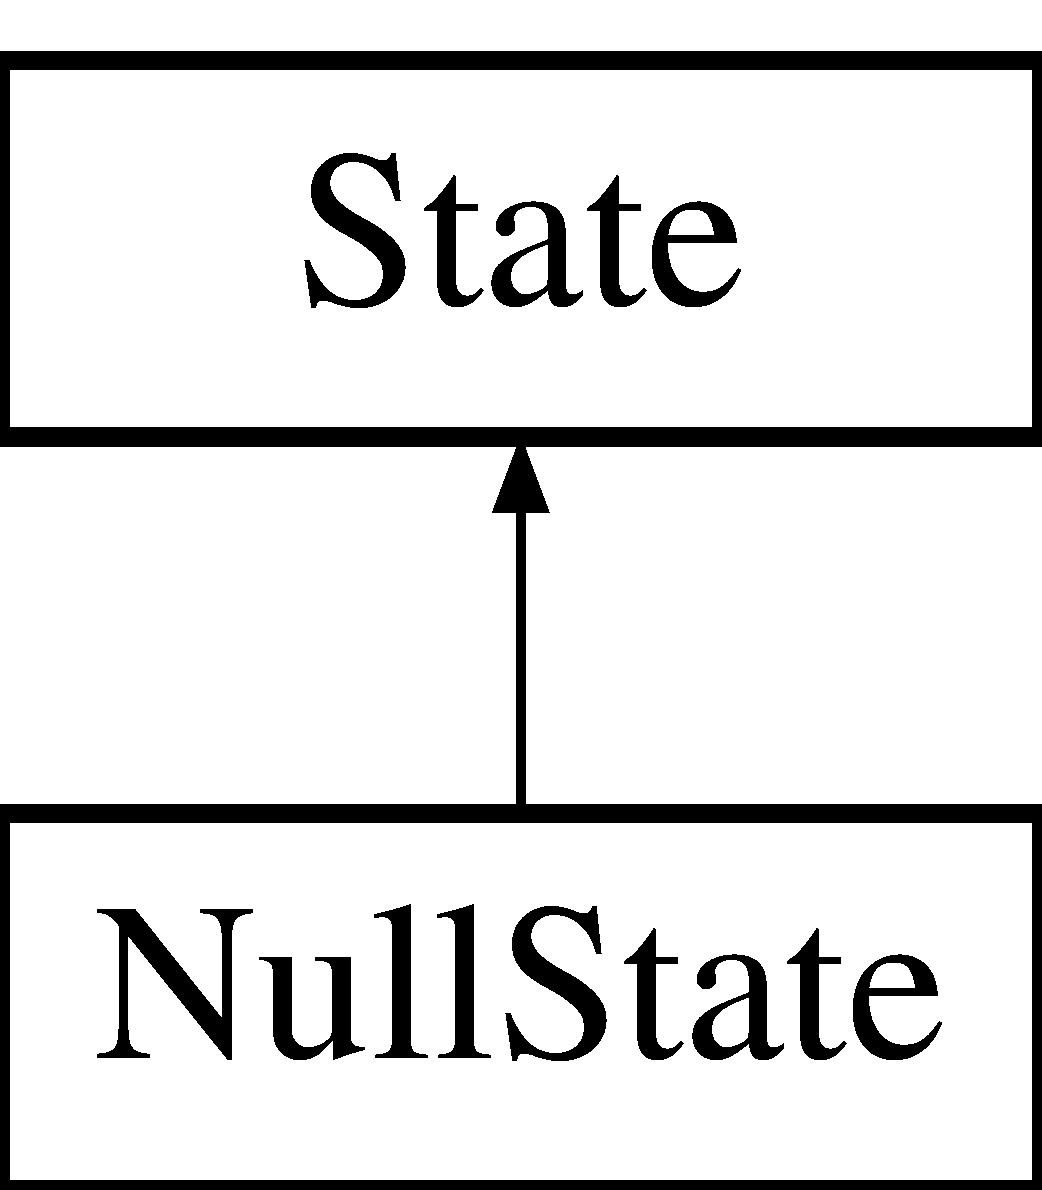
\includegraphics[height=2.000000cm]{class_null_state}
\end{center}
\end{figure}
\subsection*{Fonctions membres publiques}
\begin{DoxyCompactItemize}
\item 
\hyperlink{class_null_state_a16b8bc7f006616e9c057ddf2b1ec811d}{Null\-State} (\hyperlink{class_player}{Player} $\ast$p)
\begin{DoxyCompactList}\small\item\em Constructeur, crée un Etat\-Null à l'aide du constructeur de \hyperlink{class_state}{State} avec un Joueur en paramètre. \end{DoxyCompactList}\item 
\hyperlink{class_null_state_a3d286ab0ced8da71c8729871d1bd3aae}{$\sim$\-Null\-State} ()
\begin{DoxyCompactList}\small\item\em Destructeur de l'objet \hyperlink{class_null_state}{Null\-State}. \end{DoxyCompactList}\item 
void \hyperlink{class_null_state_a3c51a85d1d0273b7f7db4ed20672c68c}{in\-Game} ()
\begin{DoxyCompactList}\small\item\em Définition de la procédure virtuelle, pas d'effet dans cet Etat là \end{DoxyCompactList}\item 
void \hyperlink{class_null_state_a04825452cd1018dec2525609a3079aff}{check} ()
\begin{DoxyCompactList}\small\item\em Définition de la procédure virtuelle, pas d'effet dans cet Etat là \end{DoxyCompactList}\item 
void \hyperlink{class_null_state_a2bc6da41f64658fb9f733f6b23f0e499}{check\-Mate} ()
\begin{DoxyCompactList}\small\item\em Définition de la procédure virtuelle, pas d'effet dans cet Etat là \end{DoxyCompactList}\item 
void \hyperlink{class_null_state_a9a735f7e4cbf7c3439208f9bb90b649d}{game\-Null} ()
\begin{DoxyCompactList}\small\item\em Définition de la procédure virtuelle, pas d'effet dans cet Etat là \end{DoxyCompactList}\item 
void \hyperlink{class_null_state_a73b1449815c3770ac24e56fa885a7961}{game\-End} ()
\begin{DoxyCompactList}\small\item\em Définition de la procédure virtuelle, transition vers l'état End\-Game. \end{DoxyCompactList}\item 
void \hyperlink{class_null_state_a5a2b2f419bba204759bf344c8b7710d0}{print} ()
\begin{DoxyCompactList}\small\item\em Définition de la procédure virtuelle, affiche l'état \hyperlink{class_null_state}{Null\-State}. \end{DoxyCompactList}\item 
bool \hyperlink{class_null_state_a8da9c3d889ff161f893d5522a89567a5}{ischeck} ()
\begin{DoxyCompactList}\small\item\em procédure virtuelle permettant de savoir s'il se trouve en position d'echec \end{DoxyCompactList}\item 
bool \hyperlink{class_null_state_a0b43994870d835258a68300d710992ac}{is\-Check\-Mate} ()
\begin{DoxyCompactList}\small\item\em procédure virtuelle permettant de savoir s'il se trouve en position d'echec et mate \end{DoxyCompactList}\item 
bool \hyperlink{class_null_state_a0aa0845d4f2ce4f86749bd73edb8c8da}{isnulle} ()
\begin{DoxyCompactList}\small\item\em procédure virtuelle permettant de savoir s'il se trouve en position nulle \end{DoxyCompactList}\end{DoxyCompactItemize}
\subsection*{Membres hérités additionnels}


\subsection{Documentation des constructeurs et destructeur}
\hypertarget{class_null_state_a16b8bc7f006616e9c057ddf2b1ec811d}{\index{Null\-State@{Null\-State}!Null\-State@{Null\-State}}
\index{Null\-State@{Null\-State}!NullState@{Null\-State}}
\subsubsection[{Null\-State}]{\setlength{\rightskip}{0pt plus 5cm}Null\-State\-::\-Null\-State (
\begin{DoxyParamCaption}
\item[{{\bf Player} $\ast$}]{p}
\end{DoxyParamCaption}
)}}\label{class_null_state_a16b8bc7f006616e9c057ddf2b1ec811d}


Constructeur, crée un Etat\-Null à l'aide du constructeur de \hyperlink{class_state}{State} avec un Joueur en paramètre. 


\begin{DoxyParams}{Paramètres}
{\em p} & \\
\hline
\end{DoxyParams}
\hypertarget{class_null_state_a3d286ab0ced8da71c8729871d1bd3aae}{\index{Null\-State@{Null\-State}!$\sim$\-Null\-State@{$\sim$\-Null\-State}}
\index{$\sim$\-Null\-State@{$\sim$\-Null\-State}!NullState@{Null\-State}}
\subsubsection[{$\sim$\-Null\-State}]{\setlength{\rightskip}{0pt plus 5cm}Null\-State\-::$\sim$\-Null\-State (
\begin{DoxyParamCaption}
{}
\end{DoxyParamCaption}
)}}\label{class_null_state_a3d286ab0ced8da71c8729871d1bd3aae}


Destructeur de l'objet \hyperlink{class_null_state}{Null\-State}. 



\subsection{Documentation des fonctions membres}
\hypertarget{class_null_state_a04825452cd1018dec2525609a3079aff}{\index{Null\-State@{Null\-State}!check@{check}}
\index{check@{check}!NullState@{Null\-State}}
\subsubsection[{check}]{\setlength{\rightskip}{0pt plus 5cm}void Null\-State\-::check (
\begin{DoxyParamCaption}
{}
\end{DoxyParamCaption}
)\hspace{0.3cm}{\ttfamily [virtual]}}}\label{class_null_state_a04825452cd1018dec2525609a3079aff}


Définition de la procédure virtuelle, pas d'effet dans cet Etat là 



Implémente \hyperlink{class_state_a321fd726bbefc35fedbbf001d2a37021}{State}.

\hypertarget{class_null_state_a2bc6da41f64658fb9f733f6b23f0e499}{\index{Null\-State@{Null\-State}!check\-Mate@{check\-Mate}}
\index{check\-Mate@{check\-Mate}!NullState@{Null\-State}}
\subsubsection[{check\-Mate}]{\setlength{\rightskip}{0pt plus 5cm}void Null\-State\-::check\-Mate (
\begin{DoxyParamCaption}
{}
\end{DoxyParamCaption}
)\hspace{0.3cm}{\ttfamily [virtual]}}}\label{class_null_state_a2bc6da41f64658fb9f733f6b23f0e499}


Définition de la procédure virtuelle, pas d'effet dans cet Etat là 



Implémente \hyperlink{class_state_aa2b89ec92ecd4f6271269fe4b8ccc790}{State}.

\hypertarget{class_null_state_a73b1449815c3770ac24e56fa885a7961}{\index{Null\-State@{Null\-State}!game\-End@{game\-End}}
\index{game\-End@{game\-End}!NullState@{Null\-State}}
\subsubsection[{game\-End}]{\setlength{\rightskip}{0pt plus 5cm}void Null\-State\-::game\-End (
\begin{DoxyParamCaption}
{}
\end{DoxyParamCaption}
)\hspace{0.3cm}{\ttfamily [virtual]}}}\label{class_null_state_a73b1449815c3770ac24e56fa885a7961}


Définition de la procédure virtuelle, transition vers l'état End\-Game. 



Implémente \hyperlink{class_state_a5117e1f9bf06e17b4b0277838fe39bd8}{State}.

\hypertarget{class_null_state_a9a735f7e4cbf7c3439208f9bb90b649d}{\index{Null\-State@{Null\-State}!game\-Null@{game\-Null}}
\index{game\-Null@{game\-Null}!NullState@{Null\-State}}
\subsubsection[{game\-Null}]{\setlength{\rightskip}{0pt plus 5cm}void Null\-State\-::game\-Null (
\begin{DoxyParamCaption}
{}
\end{DoxyParamCaption}
)\hspace{0.3cm}{\ttfamily [virtual]}}}\label{class_null_state_a9a735f7e4cbf7c3439208f9bb90b649d}


Définition de la procédure virtuelle, pas d'effet dans cet Etat là 



Implémente \hyperlink{class_state_ad5b7fe10b2c30243f36d7d0950c50d43}{State}.

\hypertarget{class_null_state_a3c51a85d1d0273b7f7db4ed20672c68c}{\index{Null\-State@{Null\-State}!in\-Game@{in\-Game}}
\index{in\-Game@{in\-Game}!NullState@{Null\-State}}
\subsubsection[{in\-Game}]{\setlength{\rightskip}{0pt plus 5cm}void Null\-State\-::in\-Game (
\begin{DoxyParamCaption}
{}
\end{DoxyParamCaption}
)\hspace{0.3cm}{\ttfamily [virtual]}}}\label{class_null_state_a3c51a85d1d0273b7f7db4ed20672c68c}


Définition de la procédure virtuelle, pas d'effet dans cet Etat là 



Implémente \hyperlink{class_state_a738b04d6e0c12a39bf96a2a7159202d8}{State}.

\hypertarget{class_null_state_a8da9c3d889ff161f893d5522a89567a5}{\index{Null\-State@{Null\-State}!ischeck@{ischeck}}
\index{ischeck@{ischeck}!NullState@{Null\-State}}
\subsubsection[{ischeck}]{\setlength{\rightskip}{0pt plus 5cm}bool Null\-State\-::ischeck (
\begin{DoxyParamCaption}
{}
\end{DoxyParamCaption}
)\hspace{0.3cm}{\ttfamily [virtual]}}}\label{class_null_state_a8da9c3d889ff161f893d5522a89567a5}


procédure virtuelle permettant de savoir s'il se trouve en position d'echec 



Implémente \hyperlink{class_state_ad2d7084c507d8d20be2e772d953129fb}{State}.

\hypertarget{class_null_state_a0b43994870d835258a68300d710992ac}{\index{Null\-State@{Null\-State}!is\-Check\-Mate@{is\-Check\-Mate}}
\index{is\-Check\-Mate@{is\-Check\-Mate}!NullState@{Null\-State}}
\subsubsection[{is\-Check\-Mate}]{\setlength{\rightskip}{0pt plus 5cm}bool Null\-State\-::is\-Check\-Mate (
\begin{DoxyParamCaption}
{}
\end{DoxyParamCaption}
)\hspace{0.3cm}{\ttfamily [virtual]}}}\label{class_null_state_a0b43994870d835258a68300d710992ac}


procédure virtuelle permettant de savoir s'il se trouve en position d'echec et mate 



Implémente \hyperlink{class_state_ac67ccfcdc2d3e9fbe6d05961416ffeda}{State}.

\hypertarget{class_null_state_a0aa0845d4f2ce4f86749bd73edb8c8da}{\index{Null\-State@{Null\-State}!isnulle@{isnulle}}
\index{isnulle@{isnulle}!NullState@{Null\-State}}
\subsubsection[{isnulle}]{\setlength{\rightskip}{0pt plus 5cm}bool Null\-State\-::isnulle (
\begin{DoxyParamCaption}
{}
\end{DoxyParamCaption}
)\hspace{0.3cm}{\ttfamily [virtual]}}}\label{class_null_state_a0aa0845d4f2ce4f86749bd73edb8c8da}


procédure virtuelle permettant de savoir s'il se trouve en position nulle 



Implémente \hyperlink{class_state_a869f2ebfad7e60719df5f89a613adee1}{State}.

\hypertarget{class_null_state_a5a2b2f419bba204759bf344c8b7710d0}{\index{Null\-State@{Null\-State}!print@{print}}
\index{print@{print}!NullState@{Null\-State}}
\subsubsection[{print}]{\setlength{\rightskip}{0pt plus 5cm}void Null\-State\-::print (
\begin{DoxyParamCaption}
{}
\end{DoxyParamCaption}
)\hspace{0.3cm}{\ttfamily [virtual]}}}\label{class_null_state_a5a2b2f419bba204759bf344c8b7710d0}


Définition de la procédure virtuelle, affiche l'état \hyperlink{class_null_state}{Null\-State}. 



Implémente \hyperlink{class_state_a95a537bb55b9118b23d5bed88ba3b335}{State}.



La documentation de cette classe a été générée à partir des fichiers suivants \-:\begin{DoxyCompactItemize}
\item 
src/\hyperlink{_state_8hpp}{State.\-hpp}\item 
src/\hyperlink{_state_8cpp}{State.\-cpp}\end{DoxyCompactItemize}

\hypertarget{class_object_pool}{\section{Référence de la classe Object\-Pool}
\label{class_object_pool}\index{Object\-Pool@{Object\-Pool}}
}


{\ttfamily \#include $<$Object\-Pool.\-hpp$>$}

\subsection*{Fonctions membres publiques}
\begin{DoxyCompactItemize}
\item 
\hyperlink{class_object_pool_ad6a851944917327bd1c035f9a81e0684}{Object\-Pool} ()
\begin{DoxyCompactList}\small\item\em Constructeur, crée un objet \hyperlink{class_object_pool}{Object\-Pool}. \end{DoxyCompactList}\item 
\hyperlink{class_object_pool_ae45acbed251b192f83bc68ef277a7a3f}{$\sim$\-Object\-Pool} ()
\begin{DoxyCompactList}\small\item\em Destructeur. \end{DoxyCompactList}\item 
\hyperlink{class_piece}{Piece} $\ast$ \hyperlink{class_object_pool_aa6b45de56e448971193590ec18269ca0}{pick\-Piece} (unsigned int ind\-Piece)
\begin{DoxyCompactList}\small\item\em permet de prendre un objet dans la pool \end{DoxyCompactList}\item 
void \hyperlink{class_object_pool_a6f4c72edf13fadf5d873be5ef6f27cd5}{put\-Piece} (\hyperlink{class_piece}{Piece} $\ast$piece, unsigned int ind\-Piece)
\begin{DoxyCompactList}\small\item\em permet de remettre un objet dans la pool \end{DoxyCompactList}\item 
\hyperlink{class_piece}{Piece} $\ast$$\ast$ \hyperlink{class_object_pool_af9f18a929a7de70525a18bf1622bb68c}{get\-Pool} ()
\begin{DoxyCompactList}\small\item\em getter de l'attribut \-\_\-pool \end{DoxyCompactList}\end{DoxyCompactItemize}


\subsection{Documentation des constructeurs et destructeur}
\hypertarget{class_object_pool_ad6a851944917327bd1c035f9a81e0684}{\index{Object\-Pool@{Object\-Pool}!Object\-Pool@{Object\-Pool}}
\index{Object\-Pool@{Object\-Pool}!ObjectPool@{Object\-Pool}}
\subsubsection[{Object\-Pool}]{\setlength{\rightskip}{0pt plus 5cm}Object\-Pool\-::\-Object\-Pool (
\begin{DoxyParamCaption}
{}
\end{DoxyParamCaption}
)}}\label{class_object_pool_ad6a851944917327bd1c035f9a81e0684}


Constructeur, crée un objet \hyperlink{class_object_pool}{Object\-Pool}. 

\hypertarget{class_object_pool_ae45acbed251b192f83bc68ef277a7a3f}{\index{Object\-Pool@{Object\-Pool}!$\sim$\-Object\-Pool@{$\sim$\-Object\-Pool}}
\index{$\sim$\-Object\-Pool@{$\sim$\-Object\-Pool}!ObjectPool@{Object\-Pool}}
\subsubsection[{$\sim$\-Object\-Pool}]{\setlength{\rightskip}{0pt plus 5cm}Object\-Pool\-::$\sim$\-Object\-Pool (
\begin{DoxyParamCaption}
{}
\end{DoxyParamCaption}
)}}\label{class_object_pool_ae45acbed251b192f83bc68ef277a7a3f}


Destructeur. 



\subsection{Documentation des fonctions membres}
\hypertarget{class_object_pool_af9f18a929a7de70525a18bf1622bb68c}{\index{Object\-Pool@{Object\-Pool}!get\-Pool@{get\-Pool}}
\index{get\-Pool@{get\-Pool}!ObjectPool@{Object\-Pool}}
\subsubsection[{get\-Pool}]{\setlength{\rightskip}{0pt plus 5cm}{\bf Piece} $\ast$$\ast$ Object\-Pool\-::get\-Pool (
\begin{DoxyParamCaption}
{}
\end{DoxyParamCaption}
)}}\label{class_object_pool_af9f18a929a7de70525a18bf1622bb68c}


getter de l'attribut \-\_\-pool 

\begin{DoxyReturn}{Renvoie}
Piece$\ast$ 
\end{DoxyReturn}
\hypertarget{class_object_pool_aa6b45de56e448971193590ec18269ca0}{\index{Object\-Pool@{Object\-Pool}!pick\-Piece@{pick\-Piece}}
\index{pick\-Piece@{pick\-Piece}!ObjectPool@{Object\-Pool}}
\subsubsection[{pick\-Piece}]{\setlength{\rightskip}{0pt plus 5cm}{\bf Piece} $\ast$ Object\-Pool\-::pick\-Piece (
\begin{DoxyParamCaption}
\item[{unsigned int}]{ind\-Piece}
\end{DoxyParamCaption}
)}}\label{class_object_pool_aa6b45de56e448971193590ec18269ca0}


permet de prendre un objet dans la pool 


\begin{DoxyParams}{Paramètres}
{\em unsigned} & int, indice de la pool permettant d'enlever la Piece$\ast$ à cet indice \\
\hline
\end{DoxyParams}
\begin{DoxyReturn}{Renvoie}
Piece$\ast$, pointeur de la pièce sortante 
\end{DoxyReturn}
\hypertarget{class_object_pool_a6f4c72edf13fadf5d873be5ef6f27cd5}{\index{Object\-Pool@{Object\-Pool}!put\-Piece@{put\-Piece}}
\index{put\-Piece@{put\-Piece}!ObjectPool@{Object\-Pool}}
\subsubsection[{put\-Piece}]{\setlength{\rightskip}{0pt plus 5cm}void Object\-Pool\-::put\-Piece (
\begin{DoxyParamCaption}
\item[{{\bf Piece} $\ast$}]{piece, }
\item[{unsigned int}]{ind\-Piece}
\end{DoxyParamCaption}
)}}\label{class_object_pool_a6f4c72edf13fadf5d873be5ef6f27cd5}


permet de remettre un objet dans la pool 


\begin{DoxyParams}{Paramètres}
{\em Piece$\ast$,pointeur} & de la pièce à remettre dans la pool (en fin de partie) \\
\hline
{\em unsigned} & int, indice de la pool permettant de remettre la Piece$\ast$ à cet indice \\
\hline
\end{DoxyParams}


La documentation de cette classe a été générée à partir des fichiers suivants \-:\begin{DoxyCompactItemize}
\item 
src/\hyperlink{_object_pool_8hpp}{Object\-Pool.\-hpp}\item 
src/\hyperlink{_object_pool_8cpp}{Object\-Pool.\-cpp}\end{DoxyCompactItemize}

\hypertarget{class_piece}{\section{Référence de la classe Piece}
\label{class_piece}\index{Piece@{Piece}}
}


Classe abstaite de \hyperlink{class_piece}{Piece}.  




{\ttfamily \#include $<$Piece.\-hpp$>$}

Graphe d'héritage de Piece\-:\begin{figure}[H]
\begin{center}
\leavevmode
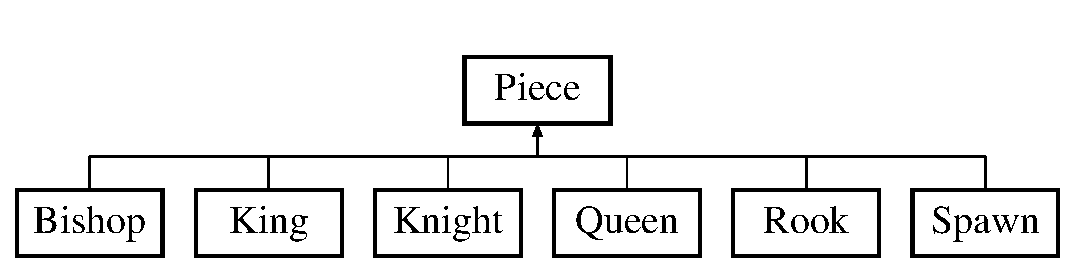
\includegraphics[height=2.000000cm]{class_piece}
\end{center}
\end{figure}
\subsection*{Fonctions membres publiques}
\begin{DoxyCompactItemize}
\item 
\hyperlink{class_piece_ac57de5803bbad829b143bc7268267dc1}{Piece} ()
\begin{DoxyCompactList}\small\item\em Constructeur vide, crée une pièce. \end{DoxyCompactList}\item 
\hyperlink{class_piece_a26c8c5a537f1733833787820d3f1ff01}{Piece} (unsigned int x, unsigned int y)
\begin{DoxyCompactList}\small\item\em Constructeur, crée une pièce. \end{DoxyCompactList}\item 
virtual \hyperlink{class_piece_a5d7a4f6bade94cb33b6f634de8aa7918}{$\sim$\-Piece} ()
\begin{DoxyCompactList}\small\item\em Destructeur de \hyperlink{class_piece}{Piece}. \end{DoxyCompactList}\item 
\hyperlink{class_cell}{Cell} $\ast$ \hyperlink{class_piece_a91fddbcc85fe9fbbca1897079ce9b9e5}{get\-Square} ()
\begin{DoxyCompactList}\small\item\em de Getter l'attribut square \end{DoxyCompactList}\item 
void \hyperlink{class_piece_af405feca349d71dfacb20b128c3cc686}{set\-Square} (\hyperlink{class_cell}{Cell} $\ast$new\-Cell)
\begin{DoxyCompactList}\small\item\em Setter de l'attribut square. \end{DoxyCompactList}\item 
bool \hyperlink{class_piece_a9f6a89d6fd5ae865af73c2220d1a5839}{is\-Alive} ()
\begin{DoxyCompactList}\small\item\em Getter de l'attribut alive. \end{DoxyCompactList}\item 
void \hyperlink{class_piece_ad4161cd37efb373e08b50cdf43b07b5f}{set\-Alive} (bool new\-Alive)
\begin{DoxyCompactList}\small\item\em Setter de l'attribut alive. \end{DoxyCompactList}\item 
std\-::string \hyperlink{class_piece_ab0b61a2a0f2f3d977b4b1946ab328f2b}{get\-Label} ()
\begin{DoxyCompactList}\small\item\em Getter l'attribut label. \end{DoxyCompactList}\item 
void \hyperlink{class_piece_ae9c47c1e15caf3ecf060c274aec62820}{print\-Piece} ()
\begin{DoxyCompactList}\small\item\em procédure permettant d'afficher les coordonnées de la case sur laquelle se trouve la pièce \end{DoxyCompactList}\item 
virtual void \hyperlink{class_piece_ae721b5ed94376fd4e7d348d36739ed4d}{movement} ()
\begin{DoxyCompactList}\small\item\em procédure virtuelle mettant à jour les cases possibles pour un déplacement de la pièce \end{DoxyCompactList}\item 
std\-::vector$<$ std\-::vector$<$ \hyperlink{class_cell}{Cell} $\ast$ $>$ $>$ \hyperlink{class_piece_af2a3be14e4732ac3f09a84a9cbefbf5b}{get\-Movements} ()
\begin{DoxyCompactList}\small\item\em Getter de l'attribut movements. \end{DoxyCompactList}\end{DoxyCompactItemize}
\subsection*{Attributs protégés}
\begin{DoxyCompactItemize}
\item 
\hyperlink{class_cell}{Cell} $\ast$ \hyperlink{class_piece_a1e38a3d73f5f7171eca664a77c7aaeff}{square}
\item 
bool \hyperlink{class_piece_a8b3c2f812ead74ba513f521e63f767f9}{alive}
\item 
std\-::vector$<$ std\-::vector$<$ \hyperlink{class_cell}{Cell} $\ast$ $>$ $>$ \hyperlink{class_piece_a022b28159d944243023804a678d7024f}{movements}
\item 
std\-::string \hyperlink{class_piece_aec026f7ca20120f0b635591de2f86662}{label}
\end{DoxyCompactItemize}


\subsection{Description détaillée}
Classe abstaite de \hyperlink{class_piece}{Piece}. 

\subsection{Documentation des constructeurs et destructeur}
\hypertarget{class_piece_ac57de5803bbad829b143bc7268267dc1}{\index{Piece@{Piece}!Piece@{Piece}}
\index{Piece@{Piece}!Piece@{Piece}}
\subsubsection[{Piece}]{\setlength{\rightskip}{0pt plus 5cm}Piece\-::\-Piece (
\begin{DoxyParamCaption}
{}
\end{DoxyParamCaption}
)}}\label{class_piece_ac57de5803bbad829b143bc7268267dc1}


Constructeur vide, crée une pièce. 

\hypertarget{class_piece_a26c8c5a537f1733833787820d3f1ff01}{\index{Piece@{Piece}!Piece@{Piece}}
\index{Piece@{Piece}!Piece@{Piece}}
\subsubsection[{Piece}]{\setlength{\rightskip}{0pt plus 5cm}Piece\-::\-Piece (
\begin{DoxyParamCaption}
\item[{unsigned int}]{x, }
\item[{unsigned int}]{y}
\end{DoxyParamCaption}
)}}\label{class_piece_a26c8c5a537f1733833787820d3f1ff01}


Constructeur, crée une pièce. 


\begin{DoxyParams}{Paramètres}
{\em unsigned} & int x \\
\hline
{\em unsigned} & int y \\
\hline
\end{DoxyParams}
\hypertarget{class_piece_a5d7a4f6bade94cb33b6f634de8aa7918}{\index{Piece@{Piece}!$\sim$\-Piece@{$\sim$\-Piece}}
\index{$\sim$\-Piece@{$\sim$\-Piece}!Piece@{Piece}}
\subsubsection[{$\sim$\-Piece}]{\setlength{\rightskip}{0pt plus 5cm}Piece\-::$\sim$\-Piece (
\begin{DoxyParamCaption}
{}
\end{DoxyParamCaption}
)\hspace{0.3cm}{\ttfamily [virtual]}}}\label{class_piece_a5d7a4f6bade94cb33b6f634de8aa7918}


Destructeur de \hyperlink{class_piece}{Piece}. 



\subsection{Documentation des fonctions membres}
\hypertarget{class_piece_ab0b61a2a0f2f3d977b4b1946ab328f2b}{\index{Piece@{Piece}!get\-Label@{get\-Label}}
\index{get\-Label@{get\-Label}!Piece@{Piece}}
\subsubsection[{get\-Label}]{\setlength{\rightskip}{0pt plus 5cm}std\-::string Piece\-::get\-Label (
\begin{DoxyParamCaption}
{}
\end{DoxyParamCaption}
)}}\label{class_piece_ab0b61a2a0f2f3d977b4b1946ab328f2b}


Getter l'attribut label. 

\begin{DoxyReturn}{Renvoie}
attribut label 
\end{DoxyReturn}
\hypertarget{class_piece_af2a3be14e4732ac3f09a84a9cbefbf5b}{\index{Piece@{Piece}!get\-Movements@{get\-Movements}}
\index{get\-Movements@{get\-Movements}!Piece@{Piece}}
\subsubsection[{get\-Movements}]{\setlength{\rightskip}{0pt plus 5cm}std\-::vector$<$ std\-::vector$<$ {\bf Cell} $\ast$ $>$ $>$ Piece\-::get\-Movements (
\begin{DoxyParamCaption}
{}
\end{DoxyParamCaption}
)}}\label{class_piece_af2a3be14e4732ac3f09a84a9cbefbf5b}


Getter de l'attribut movements. 

\begin{DoxyReturn}{Renvoie}
attribut movements 
\end{DoxyReturn}
\hypertarget{class_piece_a91fddbcc85fe9fbbca1897079ce9b9e5}{\index{Piece@{Piece}!get\-Square@{get\-Square}}
\index{get\-Square@{get\-Square}!Piece@{Piece}}
\subsubsection[{get\-Square}]{\setlength{\rightskip}{0pt plus 5cm}{\bf Cell} $\ast$ Piece\-::get\-Square (
\begin{DoxyParamCaption}
{}
\end{DoxyParamCaption}
)}}\label{class_piece_a91fddbcc85fe9fbbca1897079ce9b9e5}


de Getter l'attribut square 

\begin{DoxyReturn}{Renvoie}
attribut square 
\end{DoxyReturn}
\hypertarget{class_piece_a9f6a89d6fd5ae865af73c2220d1a5839}{\index{Piece@{Piece}!is\-Alive@{is\-Alive}}
\index{is\-Alive@{is\-Alive}!Piece@{Piece}}
\subsubsection[{is\-Alive}]{\setlength{\rightskip}{0pt plus 5cm}bool Piece\-::is\-Alive (
\begin{DoxyParamCaption}
{}
\end{DoxyParamCaption}
)}}\label{class_piece_a9f6a89d6fd5ae865af73c2220d1a5839}


Getter de l'attribut alive. 

\begin{DoxyReturn}{Renvoie}
attribut alive 
\end{DoxyReturn}
\hypertarget{class_piece_ae721b5ed94376fd4e7d348d36739ed4d}{\index{Piece@{Piece}!movement@{movement}}
\index{movement@{movement}!Piece@{Piece}}
\subsubsection[{movement}]{\setlength{\rightskip}{0pt plus 5cm}void Piece\-::movement (
\begin{DoxyParamCaption}
{}
\end{DoxyParamCaption}
)\hspace{0.3cm}{\ttfamily [virtual]}}}\label{class_piece_ae721b5ed94376fd4e7d348d36739ed4d}


procédure virtuelle mettant à jour les cases possibles pour un déplacement de la pièce 



Réimplémentée dans \hyperlink{class_king_aabc0b7a9a553383e7aba11daecbbc61c}{King}, \hyperlink{class_queen_a6cf9ea1320f2ebe6fa9bb35430e63603}{Queen}, \hyperlink{class_bishop_abd25da5816a737ab64880cbaa7bd7582}{Bishop}, \hyperlink{class_knight_ab228b385a3154ecdc18fce4cc0df9cd6}{Knight}, \hyperlink{class_rook_acc6139577c8ca679a93dcfbe42b71cb3}{Rook}, et \hyperlink{class_spawn_ae176dffa40411480840c3e39cd619300}{Spawn}.

\hypertarget{class_piece_ae9c47c1e15caf3ecf060c274aec62820}{\index{Piece@{Piece}!print\-Piece@{print\-Piece}}
\index{print\-Piece@{print\-Piece}!Piece@{Piece}}
\subsubsection[{print\-Piece}]{\setlength{\rightskip}{0pt plus 5cm}void Piece\-::print\-Piece (
\begin{DoxyParamCaption}
{}
\end{DoxyParamCaption}
)}}\label{class_piece_ae9c47c1e15caf3ecf060c274aec62820}


procédure permettant d'afficher les coordonnées de la case sur laquelle se trouve la pièce 

\hypertarget{class_piece_ad4161cd37efb373e08b50cdf43b07b5f}{\index{Piece@{Piece}!set\-Alive@{set\-Alive}}
\index{set\-Alive@{set\-Alive}!Piece@{Piece}}
\subsubsection[{set\-Alive}]{\setlength{\rightskip}{0pt plus 5cm}void Piece\-::set\-Alive (
\begin{DoxyParamCaption}
\item[{bool}]{new\-Alive}
\end{DoxyParamCaption}
)}}\label{class_piece_ad4161cd37efb373e08b50cdf43b07b5f}


Setter de l'attribut alive. 


\begin{DoxyParams}{Paramètres}
{\em new\-Alive} & \\
\hline
\end{DoxyParams}
\hypertarget{class_piece_af405feca349d71dfacb20b128c3cc686}{\index{Piece@{Piece}!set\-Square@{set\-Square}}
\index{set\-Square@{set\-Square}!Piece@{Piece}}
\subsubsection[{set\-Square}]{\setlength{\rightskip}{0pt plus 5cm}void Piece\-::set\-Square (
\begin{DoxyParamCaption}
\item[{{\bf Cell} $\ast$}]{new\-Cell}
\end{DoxyParamCaption}
)}}\label{class_piece_af405feca349d71dfacb20b128c3cc686}


Setter de l'attribut square. 


\begin{DoxyParams}{Paramètres}
{\em new\-Cell} & est la nouvelle case sur laquelle est la pièce \\
\hline
\end{DoxyParams}


\subsection{Documentation des données membres}
\hypertarget{class_piece_a8b3c2f812ead74ba513f521e63f767f9}{\index{Piece@{Piece}!alive@{alive}}
\index{alive@{alive}!Piece@{Piece}}
\subsubsection[{alive}]{\setlength{\rightskip}{0pt plus 5cm}bool Piece\-::alive\hspace{0.3cm}{\ttfamily [protected]}}}\label{class_piece_a8b3c2f812ead74ba513f521e63f767f9}
\hypertarget{class_piece_aec026f7ca20120f0b635591de2f86662}{\index{Piece@{Piece}!label@{label}}
\index{label@{label}!Piece@{Piece}}
\subsubsection[{label}]{\setlength{\rightskip}{0pt plus 5cm}std\-::string Piece\-::label\hspace{0.3cm}{\ttfamily [protected]}}}\label{class_piece_aec026f7ca20120f0b635591de2f86662}
\hypertarget{class_piece_a022b28159d944243023804a678d7024f}{\index{Piece@{Piece}!movements@{movements}}
\index{movements@{movements}!Piece@{Piece}}
\subsubsection[{movements}]{\setlength{\rightskip}{0pt plus 5cm}std\-::vector$<$ std\-::vector$<${\bf Cell}$\ast$$>$ $>$ Piece\-::movements\hspace{0.3cm}{\ttfamily [protected]}}}\label{class_piece_a022b28159d944243023804a678d7024f}
\hypertarget{class_piece_a1e38a3d73f5f7171eca664a77c7aaeff}{\index{Piece@{Piece}!square@{square}}
\index{square@{square}!Piece@{Piece}}
\subsubsection[{square}]{\setlength{\rightskip}{0pt plus 5cm}{\bf Cell}$\ast$ Piece\-::square\hspace{0.3cm}{\ttfamily [protected]}}}\label{class_piece_a1e38a3d73f5f7171eca664a77c7aaeff}


La documentation de cette classe a été générée à partir des fichiers suivants \-:\begin{DoxyCompactItemize}
\item 
src/\hyperlink{_piece_8hpp}{Piece.\-hpp}\item 
src/\hyperlink{_piece_8cpp}{Piece.\-cpp}\end{DoxyCompactItemize}

\hypertarget{class_player}{\section{Référence de la classe Player}
\label{class_player}\index{Player@{Player}}
}


{\ttfamily \#include $<$Player.\-hpp$>$}

\subsection*{Fonctions membres publiques}
\begin{DoxyCompactItemize}
\item 
\hyperlink{class_player_a06ca07f2ce539e4b458437857a720718}{Player} (std\-::string name, std\-::string color)
\begin{DoxyCompactList}\small\item\em Destructeur de \hyperlink{class_player}{Player}. \end{DoxyCompactList}\item 
\hyperlink{class_player_a749d2c00e1fe0f5c2746f7505a58c062}{$\sim$\-Player} ()
\begin{DoxyCompactList}\small\item\em Destructeur de \hyperlink{class_player}{Player}. \end{DoxyCompactList}\item 
void \hyperlink{class_player_ac587f5febaceec87ddefbaf78f74539d}{in\-Game} ()
\begin{DoxyCompactList}\small\item\em Permet de passer le joueur en état de jeu \char`\"{}normal\char`\"{}. \end{DoxyCompactList}\item 
void \hyperlink{class_player_adf4962f4f2b134085f1e26809cf42680}{check} ()
\begin{DoxyCompactList}\small\item\em Permet de passer le joueur en état d'Echec. \end{DoxyCompactList}\item 
void \hyperlink{class_player_ab9d193b41e8553470f7af7c18abe3ecc}{check\-Mate} ()
\begin{DoxyCompactList}\small\item\em Permet de passer le joueur en état d'Echec et Mat. \end{DoxyCompactList}\item 
void \hyperlink{class_player_ab2f4e51ebb224662fd6e2aac37ed7a05}{game\-Null} ()
\begin{DoxyCompactList}\small\item\em Permet de passer le joueur en état de partie nulle. \end{DoxyCompactList}\item 
void \hyperlink{class_player_a3e67b9ce45f196d24395b9a44cb3e140}{game\-End} ()
\begin{DoxyCompactList}\small\item\em Permet de passer le joueur en état de partie finie. \end{DoxyCompactList}\item 
void \hyperlink{class_player_a4fda4bd6b5fa84d436a7592e4faebe92}{print\-State} ()
\begin{DoxyCompactList}\small\item\em Affiche l'état courant du joueur sur la sortie standard. \end{DoxyCompactList}\item 
void \hyperlink{class_player_ac51828429e6e1401f04677ec3f1e0769}{print\-Pieces} ()
\begin{DoxyCompactList}\small\item\em Affiche l'ensemble des pièces encore en vie avec leurs coordonnées respectives. \end{DoxyCompactList}\item 
\hyperlink{class_piece}{Piece} $\ast$ \hyperlink{class_player_a777c790075ce371af98eaf6e40f2a726}{select\-Piece} (unsigned int x, unsigned int y)
\begin{DoxyCompactList}\small\item\em Permet au joueur de selectionner une pièce qu'il possède. \end{DoxyCompactList}\item 
std\-::string \hyperlink{class_player_af1aa472885d589516f483e26e786600e}{get\-Name} ()
\begin{DoxyCompactList}\small\item\em Getter de l'attribut \-\_\-name. \end{DoxyCompactList}\item 
void \hyperlink{class_player_a1b456e164e73e5cf5ffe925529fc8c2a}{set\-Name} (std\-::string new\-Name)
\begin{DoxyCompactList}\small\item\em Setter de l'attribut \-\_\-name. \end{DoxyCompactList}\item 
std\-::string \hyperlink{class_player_a3e4c06283c8cb949b338830b0d3d6abc}{get\-Color} ()
\begin{DoxyCompactList}\small\item\em Getter de l'attribut \-\_\-color. \end{DoxyCompactList}\item 
\hyperlink{class_piece}{Piece} $\ast$$\ast$ \hyperlink{class_player_a738451fc076901ecf28cae81c7604e2a}{get\-Pieces} ()
\begin{DoxyCompactList}\small\item\em Getter de l'attribut \-\_\-pieces. \end{DoxyCompactList}\item 
\hyperlink{class_state}{State} $\ast$ \hyperlink{class_player_a1b85aeef66cdbc472caf951d25796086}{get\-State} ()
\begin{DoxyCompactList}\small\item\em Getter de l'attribut $\ast$\-\_\-state. \end{DoxyCompactList}\item 
void \hyperlink{class_player_a02d8b0f8340dc5557a01b33c4254757a}{set\-State} (\hyperlink{class_state}{State} $\ast$new\-State)
\begin{DoxyCompactList}\small\item\em Setter de l'attribut $\ast$\-\_\-state. \end{DoxyCompactList}\item 
\hyperlink{class_state}{State} $\ast$ \hyperlink{class_player_a98676a7d1647ac6db50507850fab1d92}{get\-Game\-State} ()
\begin{DoxyCompactList}\small\item\em Getter de l'attribut $\ast$game\-State. \end{DoxyCompactList}\item 
\hyperlink{class_state}{State} $\ast$ \hyperlink{class_player_a24f6a87b0480786ba2f966bc88d15195}{get\-Check\-State} ()
\begin{DoxyCompactList}\small\item\em Getter de l'attribut $\ast$\-\_\-check\-State. \end{DoxyCompactList}\item 
\hyperlink{class_state}{State} $\ast$ \hyperlink{class_player_abd42a23982b38a78bf66fe627d73b4cc}{get\-Mate\-State} ()
\begin{DoxyCompactList}\small\item\em Getter de l'attribut $\ast$\-\_\-mate\-State. \end{DoxyCompactList}\item 
\hyperlink{class_state}{State} $\ast$ \hyperlink{class_player_a121812f4c5a5e913f31187b90f378aa7}{get\-Null\-State} ()
\begin{DoxyCompactList}\small\item\em Getter de l'attribut $\ast$\-\_\-null\-State. \end{DoxyCompactList}\item 
\hyperlink{class_state}{State} $\ast$ \hyperlink{class_player_af8a9597bb9da1dcd21cb849ca519802b}{get\-End\-State} ()
\begin{DoxyCompactList}\small\item\em Getter de l'attribut $\ast$\-\_\-end\-State. \end{DoxyCompactList}\item 
\hyperlink{class_piece}{Piece} $\ast$ \hyperlink{class_player_a40125b547cb5a3c25f17a34364e6c411}{get\-King} ()
\begin{DoxyCompactList}\small\item\em permet de retourner la piece roi \end{DoxyCompactList}\item 
bool \hyperlink{class_player_aa9c151901c3fae3ead5dc7d82e9a7f88}{is\-Check\-Mate} ()
\begin{DoxyCompactList}\small\item\em permet de savoir si le joueur se trouve en en checkmate \end{DoxyCompactList}\item 
bool \hyperlink{class_player_aa8d4b069eedca62c2b8d5243db8689db}{ischeck} ()
\begin{DoxyCompactList}\small\item\em permet de savoir si le joueur se trouve en en check \end{DoxyCompactList}\item 
bool \hyperlink{class_player_a363d24fe41c4d6b0faad5f90f53a2114}{isnulle} ()
\begin{DoxyCompactList}\small\item\em permet de savoir si le joueur se trouve en en partie nulle \end{DoxyCompactList}\end{DoxyCompactItemize}


\subsection{Documentation des constructeurs et destructeur}
\hypertarget{class_player_a06ca07f2ce539e4b458437857a720718}{\index{Player@{Player}!Player@{Player}}
\index{Player@{Player}!Player@{Player}}
\subsubsection[{Player}]{\setlength{\rightskip}{0pt plus 5cm}Player\-::\-Player (
\begin{DoxyParamCaption}
\item[{std\-::string}]{name, }
\item[{std\-::string}]{color}
\end{DoxyParamCaption}
)}}\label{class_player_a06ca07f2ce539e4b458437857a720718}


Destructeur de \hyperlink{class_player}{Player}. 


\begin{DoxyParams}{Paramètres}
{\em name,nom} & du joueur \\
\hline
\end{DoxyParams}
\hypertarget{class_player_a749d2c00e1fe0f5c2746f7505a58c062}{\index{Player@{Player}!$\sim$\-Player@{$\sim$\-Player}}
\index{$\sim$\-Player@{$\sim$\-Player}!Player@{Player}}
\subsubsection[{$\sim$\-Player}]{\setlength{\rightskip}{0pt plus 5cm}Player\-::$\sim$\-Player (
\begin{DoxyParamCaption}
{}
\end{DoxyParamCaption}
)}}\label{class_player_a749d2c00e1fe0f5c2746f7505a58c062}


Destructeur de \hyperlink{class_player}{Player}. 



\subsection{Documentation des fonctions membres}
\hypertarget{class_player_adf4962f4f2b134085f1e26809cf42680}{\index{Player@{Player}!check@{check}}
\index{check@{check}!Player@{Player}}
\subsubsection[{check}]{\setlength{\rightskip}{0pt plus 5cm}void Player\-::check (
\begin{DoxyParamCaption}
{}
\end{DoxyParamCaption}
)}}\label{class_player_adf4962f4f2b134085f1e26809cf42680}


Permet de passer le joueur en état d'Echec. 

\hypertarget{class_player_ab9d193b41e8553470f7af7c18abe3ecc}{\index{Player@{Player}!check\-Mate@{check\-Mate}}
\index{check\-Mate@{check\-Mate}!Player@{Player}}
\subsubsection[{check\-Mate}]{\setlength{\rightskip}{0pt plus 5cm}void Player\-::check\-Mate (
\begin{DoxyParamCaption}
{}
\end{DoxyParamCaption}
)}}\label{class_player_ab9d193b41e8553470f7af7c18abe3ecc}


Permet de passer le joueur en état d'Echec et Mat. 

\hypertarget{class_player_a3e67b9ce45f196d24395b9a44cb3e140}{\index{Player@{Player}!game\-End@{game\-End}}
\index{game\-End@{game\-End}!Player@{Player}}
\subsubsection[{game\-End}]{\setlength{\rightskip}{0pt plus 5cm}void Player\-::game\-End (
\begin{DoxyParamCaption}
{}
\end{DoxyParamCaption}
)}}\label{class_player_a3e67b9ce45f196d24395b9a44cb3e140}


Permet de passer le joueur en état de partie finie. 

\hypertarget{class_player_ab2f4e51ebb224662fd6e2aac37ed7a05}{\index{Player@{Player}!game\-Null@{game\-Null}}
\index{game\-Null@{game\-Null}!Player@{Player}}
\subsubsection[{game\-Null}]{\setlength{\rightskip}{0pt plus 5cm}void Player\-::game\-Null (
\begin{DoxyParamCaption}
{}
\end{DoxyParamCaption}
)}}\label{class_player_ab2f4e51ebb224662fd6e2aac37ed7a05}


Permet de passer le joueur en état de partie nulle. 

\hypertarget{class_player_a24f6a87b0480786ba2f966bc88d15195}{\index{Player@{Player}!get\-Check\-State@{get\-Check\-State}}
\index{get\-Check\-State@{get\-Check\-State}!Player@{Player}}
\subsubsection[{get\-Check\-State}]{\setlength{\rightskip}{0pt plus 5cm}{\bf State} $\ast$ Player\-::get\-Check\-State (
\begin{DoxyParamCaption}
{}
\end{DoxyParamCaption}
)}}\label{class_player_a24f6a87b0480786ba2f966bc88d15195}


Getter de l'attribut $\ast$\-\_\-check\-State. 

\begin{DoxyReturn}{Renvoie}
attribut $\ast$\-\_\-check\-State 
\end{DoxyReturn}
\hypertarget{class_player_a3e4c06283c8cb949b338830b0d3d6abc}{\index{Player@{Player}!get\-Color@{get\-Color}}
\index{get\-Color@{get\-Color}!Player@{Player}}
\subsubsection[{get\-Color}]{\setlength{\rightskip}{0pt plus 5cm}std\-::string Player\-::get\-Color (
\begin{DoxyParamCaption}
{}
\end{DoxyParamCaption}
)}}\label{class_player_a3e4c06283c8cb949b338830b0d3d6abc}


Getter de l'attribut \-\_\-color. 

\begin{DoxyReturn}{Renvoie}
attribut \-\_\-color 
\end{DoxyReturn}
\hypertarget{class_player_af8a9597bb9da1dcd21cb849ca519802b}{\index{Player@{Player}!get\-End\-State@{get\-End\-State}}
\index{get\-End\-State@{get\-End\-State}!Player@{Player}}
\subsubsection[{get\-End\-State}]{\setlength{\rightskip}{0pt plus 5cm}{\bf State} $\ast$ Player\-::get\-End\-State (
\begin{DoxyParamCaption}
{}
\end{DoxyParamCaption}
)}}\label{class_player_af8a9597bb9da1dcd21cb849ca519802b}


Getter de l'attribut $\ast$\-\_\-end\-State. 

\begin{DoxyReturn}{Renvoie}
attribut $\ast$\-\_\-end\-State 
\end{DoxyReturn}
\hypertarget{class_player_a98676a7d1647ac6db50507850fab1d92}{\index{Player@{Player}!get\-Game\-State@{get\-Game\-State}}
\index{get\-Game\-State@{get\-Game\-State}!Player@{Player}}
\subsubsection[{get\-Game\-State}]{\setlength{\rightskip}{0pt plus 5cm}{\bf State} $\ast$ Player\-::get\-Game\-State (
\begin{DoxyParamCaption}
{}
\end{DoxyParamCaption}
)}}\label{class_player_a98676a7d1647ac6db50507850fab1d92}


Getter de l'attribut $\ast$game\-State. 

\begin{DoxyReturn}{Renvoie}
attribut $\ast$game\-State 
\end{DoxyReturn}
\hypertarget{class_player_a40125b547cb5a3c25f17a34364e6c411}{\index{Player@{Player}!get\-King@{get\-King}}
\index{get\-King@{get\-King}!Player@{Player}}
\subsubsection[{get\-King}]{\setlength{\rightskip}{0pt plus 5cm}{\bf Piece} $\ast$ Player\-::get\-King (
\begin{DoxyParamCaption}
{}
\end{DoxyParamCaption}
)}}\label{class_player_a40125b547cb5a3c25f17a34364e6c411}


permet de retourner la piece roi 

\begin{DoxyReturn}{Renvoie}
piece$\ast$ pointeur de la piece roi 
\end{DoxyReturn}
\hypertarget{class_player_abd42a23982b38a78bf66fe627d73b4cc}{\index{Player@{Player}!get\-Mate\-State@{get\-Mate\-State}}
\index{get\-Mate\-State@{get\-Mate\-State}!Player@{Player}}
\subsubsection[{get\-Mate\-State}]{\setlength{\rightskip}{0pt plus 5cm}{\bf State} $\ast$ Player\-::get\-Mate\-State (
\begin{DoxyParamCaption}
{}
\end{DoxyParamCaption}
)}}\label{class_player_abd42a23982b38a78bf66fe627d73b4cc}


Getter de l'attribut $\ast$\-\_\-mate\-State. 

\begin{DoxyReturn}{Renvoie}
attribut $\ast$\-\_\-mate\-State 
\end{DoxyReturn}
\hypertarget{class_player_af1aa472885d589516f483e26e786600e}{\index{Player@{Player}!get\-Name@{get\-Name}}
\index{get\-Name@{get\-Name}!Player@{Player}}
\subsubsection[{get\-Name}]{\setlength{\rightskip}{0pt plus 5cm}std\-::string Player\-::get\-Name (
\begin{DoxyParamCaption}
{}
\end{DoxyParamCaption}
)}}\label{class_player_af1aa472885d589516f483e26e786600e}


Getter de l'attribut \-\_\-name. 

\begin{DoxyReturn}{Renvoie}
attribut \-\_\-name 
\end{DoxyReturn}
\hypertarget{class_player_a121812f4c5a5e913f31187b90f378aa7}{\index{Player@{Player}!get\-Null\-State@{get\-Null\-State}}
\index{get\-Null\-State@{get\-Null\-State}!Player@{Player}}
\subsubsection[{get\-Null\-State}]{\setlength{\rightskip}{0pt plus 5cm}{\bf State} $\ast$ Player\-::get\-Null\-State (
\begin{DoxyParamCaption}
{}
\end{DoxyParamCaption}
)}}\label{class_player_a121812f4c5a5e913f31187b90f378aa7}


Getter de l'attribut $\ast$\-\_\-null\-State. 

\begin{DoxyReturn}{Renvoie}
attribut $\ast$\-\_\-null\-State 
\end{DoxyReturn}
\hypertarget{class_player_a738451fc076901ecf28cae81c7604e2a}{\index{Player@{Player}!get\-Pieces@{get\-Pieces}}
\index{get\-Pieces@{get\-Pieces}!Player@{Player}}
\subsubsection[{get\-Pieces}]{\setlength{\rightskip}{0pt plus 5cm}{\bf Piece} $\ast$$\ast$ Player\-::get\-Pieces (
\begin{DoxyParamCaption}
{}
\end{DoxyParamCaption}
)}}\label{class_player_a738451fc076901ecf28cae81c7604e2a}


Getter de l'attribut \-\_\-pieces. 

\begin{DoxyReturn}{Renvoie}
attribut \-\_\-pieces 
\end{DoxyReturn}
\hypertarget{class_player_a1b85aeef66cdbc472caf951d25796086}{\index{Player@{Player}!get\-State@{get\-State}}
\index{get\-State@{get\-State}!Player@{Player}}
\subsubsection[{get\-State}]{\setlength{\rightskip}{0pt plus 5cm}{\bf State} $\ast$ Player\-::get\-State (
\begin{DoxyParamCaption}
{}
\end{DoxyParamCaption}
)}}\label{class_player_a1b85aeef66cdbc472caf951d25796086}


Getter de l'attribut $\ast$\-\_\-state. 

\begin{DoxyReturn}{Renvoie}
attribut $\ast$\-\_\-state 
\end{DoxyReturn}
\hypertarget{class_player_ac587f5febaceec87ddefbaf78f74539d}{\index{Player@{Player}!in\-Game@{in\-Game}}
\index{in\-Game@{in\-Game}!Player@{Player}}
\subsubsection[{in\-Game}]{\setlength{\rightskip}{0pt plus 5cm}void Player\-::in\-Game (
\begin{DoxyParamCaption}
{}
\end{DoxyParamCaption}
)}}\label{class_player_ac587f5febaceec87ddefbaf78f74539d}


Permet de passer le joueur en état de jeu \char`\"{}normal\char`\"{}. 

\hypertarget{class_player_aa8d4b069eedca62c2b8d5243db8689db}{\index{Player@{Player}!ischeck@{ischeck}}
\index{ischeck@{ischeck}!Player@{Player}}
\subsubsection[{ischeck}]{\setlength{\rightskip}{0pt plus 5cm}bool Player\-::ischeck (
\begin{DoxyParamCaption}
{}
\end{DoxyParamCaption}
)}}\label{class_player_aa8d4b069eedca62c2b8d5243db8689db}


permet de savoir si le joueur se trouve en en check 

\begin{DoxyReturn}{Renvoie}
bool 
\end{DoxyReturn}
\hypertarget{class_player_aa9c151901c3fae3ead5dc7d82e9a7f88}{\index{Player@{Player}!is\-Check\-Mate@{is\-Check\-Mate}}
\index{is\-Check\-Mate@{is\-Check\-Mate}!Player@{Player}}
\subsubsection[{is\-Check\-Mate}]{\setlength{\rightskip}{0pt plus 5cm}bool Player\-::is\-Check\-Mate (
\begin{DoxyParamCaption}
{}
\end{DoxyParamCaption}
)}}\label{class_player_aa9c151901c3fae3ead5dc7d82e9a7f88}


permet de savoir si le joueur se trouve en en checkmate 

\begin{DoxyReturn}{Renvoie}
bool 
\end{DoxyReturn}
\hypertarget{class_player_a363d24fe41c4d6b0faad5f90f53a2114}{\index{Player@{Player}!isnulle@{isnulle}}
\index{isnulle@{isnulle}!Player@{Player}}
\subsubsection[{isnulle}]{\setlength{\rightskip}{0pt plus 5cm}bool Player\-::isnulle (
\begin{DoxyParamCaption}
{}
\end{DoxyParamCaption}
)}}\label{class_player_a363d24fe41c4d6b0faad5f90f53a2114}


permet de savoir si le joueur se trouve en en partie nulle 

\begin{DoxyReturn}{Renvoie}
bool 
\end{DoxyReturn}
\hypertarget{class_player_ac51828429e6e1401f04677ec3f1e0769}{\index{Player@{Player}!print\-Pieces@{print\-Pieces}}
\index{print\-Pieces@{print\-Pieces}!Player@{Player}}
\subsubsection[{print\-Pieces}]{\setlength{\rightskip}{0pt plus 5cm}void Player\-::print\-Pieces (
\begin{DoxyParamCaption}
{}
\end{DoxyParamCaption}
)}}\label{class_player_ac51828429e6e1401f04677ec3f1e0769}


Affiche l'ensemble des pièces encore en vie avec leurs coordonnées respectives. 

\hypertarget{class_player_a4fda4bd6b5fa84d436a7592e4faebe92}{\index{Player@{Player}!print\-State@{print\-State}}
\index{print\-State@{print\-State}!Player@{Player}}
\subsubsection[{print\-State}]{\setlength{\rightskip}{0pt plus 5cm}void Player\-::print\-State (
\begin{DoxyParamCaption}
{}
\end{DoxyParamCaption}
)}}\label{class_player_a4fda4bd6b5fa84d436a7592e4faebe92}


Affiche l'état courant du joueur sur la sortie standard. 

\hypertarget{class_player_a777c790075ce371af98eaf6e40f2a726}{\index{Player@{Player}!select\-Piece@{select\-Piece}}
\index{select\-Piece@{select\-Piece}!Player@{Player}}
\subsubsection[{select\-Piece}]{\setlength{\rightskip}{0pt plus 5cm}{\bf Piece} $\ast$ Player\-::select\-Piece (
\begin{DoxyParamCaption}
\item[{unsigned int}]{x, }
\item[{unsigned int}]{y}
\end{DoxyParamCaption}
)}}\label{class_player_a777c790075ce371af98eaf6e40f2a726}


Permet au joueur de selectionner une pièce qu'il possède. 


\begin{DoxyParams}{Paramètres}
{\em unsigned} & int x, coordonnée x de la case selectionnée \\
\hline
{\em unsigned} & int y, coordonnée y de la case selectionnée \\
\hline
\end{DoxyParams}
\begin{DoxyReturn}{Renvoie}
Piece$\ast$ pointeur de la pièce selectionnée (null si coordonnées invalides) 
\end{DoxyReturn}
\hypertarget{class_player_a1b456e164e73e5cf5ffe925529fc8c2a}{\index{Player@{Player}!set\-Name@{set\-Name}}
\index{set\-Name@{set\-Name}!Player@{Player}}
\subsubsection[{set\-Name}]{\setlength{\rightskip}{0pt plus 5cm}void Player\-::set\-Name (
\begin{DoxyParamCaption}
\item[{std\-::string}]{new\-Name}
\end{DoxyParamCaption}
)}}\label{class_player_a1b456e164e73e5cf5ffe925529fc8c2a}


Setter de l'attribut \-\_\-name. 


\begin{DoxyParams}{Paramètres}
{\em new\-Name,nouveau} & nom \\
\hline
\end{DoxyParams}
\hypertarget{class_player_a02d8b0f8340dc5557a01b33c4254757a}{\index{Player@{Player}!set\-State@{set\-State}}
\index{set\-State@{set\-State}!Player@{Player}}
\subsubsection[{set\-State}]{\setlength{\rightskip}{0pt plus 5cm}void Player\-::set\-State (
\begin{DoxyParamCaption}
\item[{{\bf State} $\ast$}]{new\-State}
\end{DoxyParamCaption}
)}}\label{class_player_a02d8b0f8340dc5557a01b33c4254757a}


Setter de l'attribut $\ast$\-\_\-state. 


\begin{DoxyParams}{Paramètres}
{\em new\-Name,nouveau} & nom \\
\hline
\end{DoxyParams}


La documentation de cette classe a été générée à partir des fichiers suivants \-:\begin{DoxyCompactItemize}
\item 
src/\hyperlink{_player_8hpp}{Player.\-hpp}\item 
src/\hyperlink{_player_8cpp}{Player.\-cpp}\end{DoxyCompactItemize}

\hypertarget{class_queen}{\section{Référence de la classe Queen}
\label{class_queen}\index{Queen@{Queen}}
}


Classe \hyperlink{class_queen}{Queen} héritant de \hyperlink{class_piece}{Piece}.  




{\ttfamily \#include $<$Piece.\-hpp$>$}

Graphe d'héritage de Queen\-:\begin{figure}[H]
\begin{center}
\leavevmode
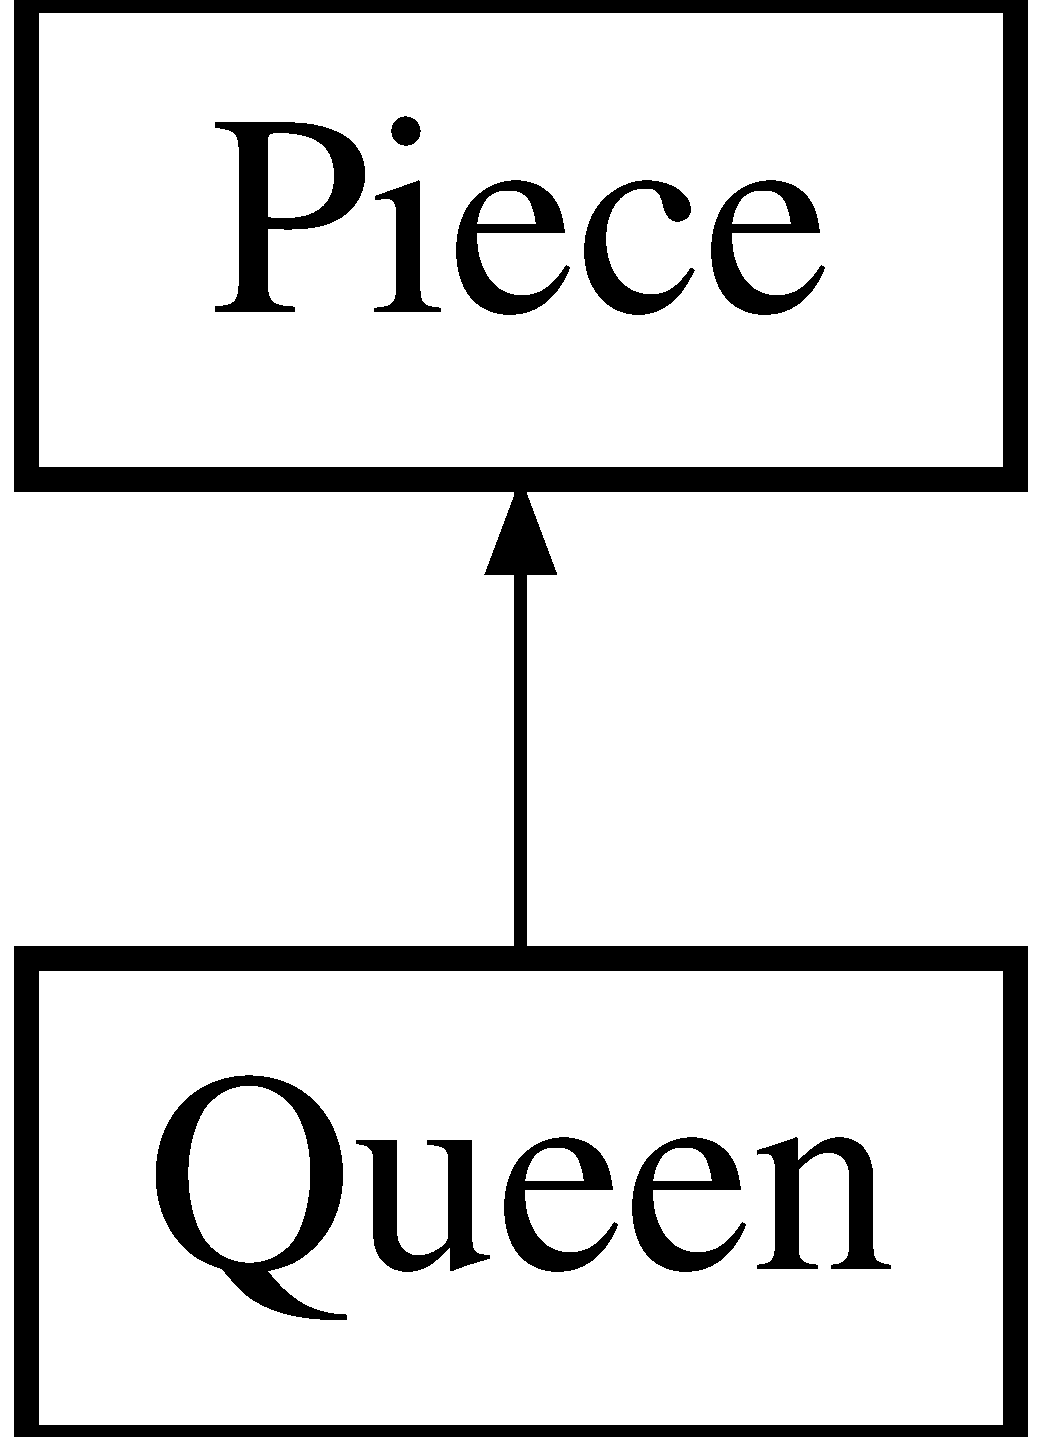
\includegraphics[height=2.000000cm]{class_queen}
\end{center}
\end{figure}
\subsection*{Fonctions membres publiques}
\begin{DoxyCompactItemize}
\item 
\hyperlink{class_queen_a90ebaca4522d07b5a662b20c09a968aa}{Queen} (unsigned int x, unsigned int y)
\begin{DoxyCompactList}\small\item\em Constructeur, crée un objet \hyperlink{class_queen}{Queen} de coordonnées x,y. \end{DoxyCompactList}\item 
\hyperlink{class_queen_aa22f6c1a49a583b549bd1f940e50721d}{$\sim$\-Queen} ()
\begin{DoxyCompactList}\small\item\em Destructeur d'un objet cavalier. \end{DoxyCompactList}\item 
virtual void \hyperlink{class_queen_a6cf9ea1320f2ebe6fa9bb35430e63603}{movement} ()
\begin{DoxyCompactList}\small\item\em procédure virtuelle permettant de mettre à jour l'attribut movements en fonction des déplacements possibles de la Dame \end{DoxyCompactList}\end{DoxyCompactItemize}
\subsection*{Membres hérités additionnels}


\subsection{Description détaillée}
Classe \hyperlink{class_queen}{Queen} héritant de \hyperlink{class_piece}{Piece}. 

\subsection{Documentation des constructeurs et destructeur}
\hypertarget{class_queen_a90ebaca4522d07b5a662b20c09a968aa}{\index{Queen@{Queen}!Queen@{Queen}}
\index{Queen@{Queen}!Queen@{Queen}}
\subsubsection[{Queen}]{\setlength{\rightskip}{0pt plus 5cm}Queen\-::\-Queen (
\begin{DoxyParamCaption}
\item[{unsigned int}]{x, }
\item[{unsigned int}]{y}
\end{DoxyParamCaption}
)}}\label{class_queen_a90ebaca4522d07b5a662b20c09a968aa}


Constructeur, crée un objet \hyperlink{class_queen}{Queen} de coordonnées x,y. 


\begin{DoxyParams}{Paramètres}
{\em unsigned} & int x \\
\hline
{\em unsigned} & int y \\
\hline
\end{DoxyParams}
\hypertarget{class_queen_aa22f6c1a49a583b549bd1f940e50721d}{\index{Queen@{Queen}!$\sim$\-Queen@{$\sim$\-Queen}}
\index{$\sim$\-Queen@{$\sim$\-Queen}!Queen@{Queen}}
\subsubsection[{$\sim$\-Queen}]{\setlength{\rightskip}{0pt plus 5cm}Queen\-::$\sim$\-Queen (
\begin{DoxyParamCaption}
{}
\end{DoxyParamCaption}
)}}\label{class_queen_aa22f6c1a49a583b549bd1f940e50721d}


Destructeur d'un objet cavalier. 



\subsection{Documentation des fonctions membres}
\hypertarget{class_queen_a6cf9ea1320f2ebe6fa9bb35430e63603}{\index{Queen@{Queen}!movement@{movement}}
\index{movement@{movement}!Queen@{Queen}}
\subsubsection[{movement}]{\setlength{\rightskip}{0pt plus 5cm}void Queen\-::movement (
\begin{DoxyParamCaption}
{}
\end{DoxyParamCaption}
)\hspace{0.3cm}{\ttfamily [virtual]}}}\label{class_queen_a6cf9ea1320f2ebe6fa9bb35430e63603}


procédure virtuelle permettant de mettre à jour l'attribut movements en fonction des déplacements possibles de la Dame 



Réimplémentée à partir de \hyperlink{class_piece_ae721b5ed94376fd4e7d348d36739ed4d}{Piece}.



La documentation de cette classe a été générée à partir des fichiers suivants \-:\begin{DoxyCompactItemize}
\item 
src/\hyperlink{_piece_8hpp}{Piece.\-hpp}\item 
src/\hyperlink{_piece_8cpp}{Piece.\-cpp}\end{DoxyCompactItemize}

\hypertarget{class_rook}{\section{Référence de la classe Rook}
\label{class_rook}\index{Rook@{Rook}}
}


Classe \hyperlink{class_rook}{Rook} héritant de \hyperlink{class_piece}{Piece}.  




{\ttfamily \#include $<$Piece.\-hpp$>$}

Graphe d'héritage de Rook\-:\begin{figure}[H]
\begin{center}
\leavevmode
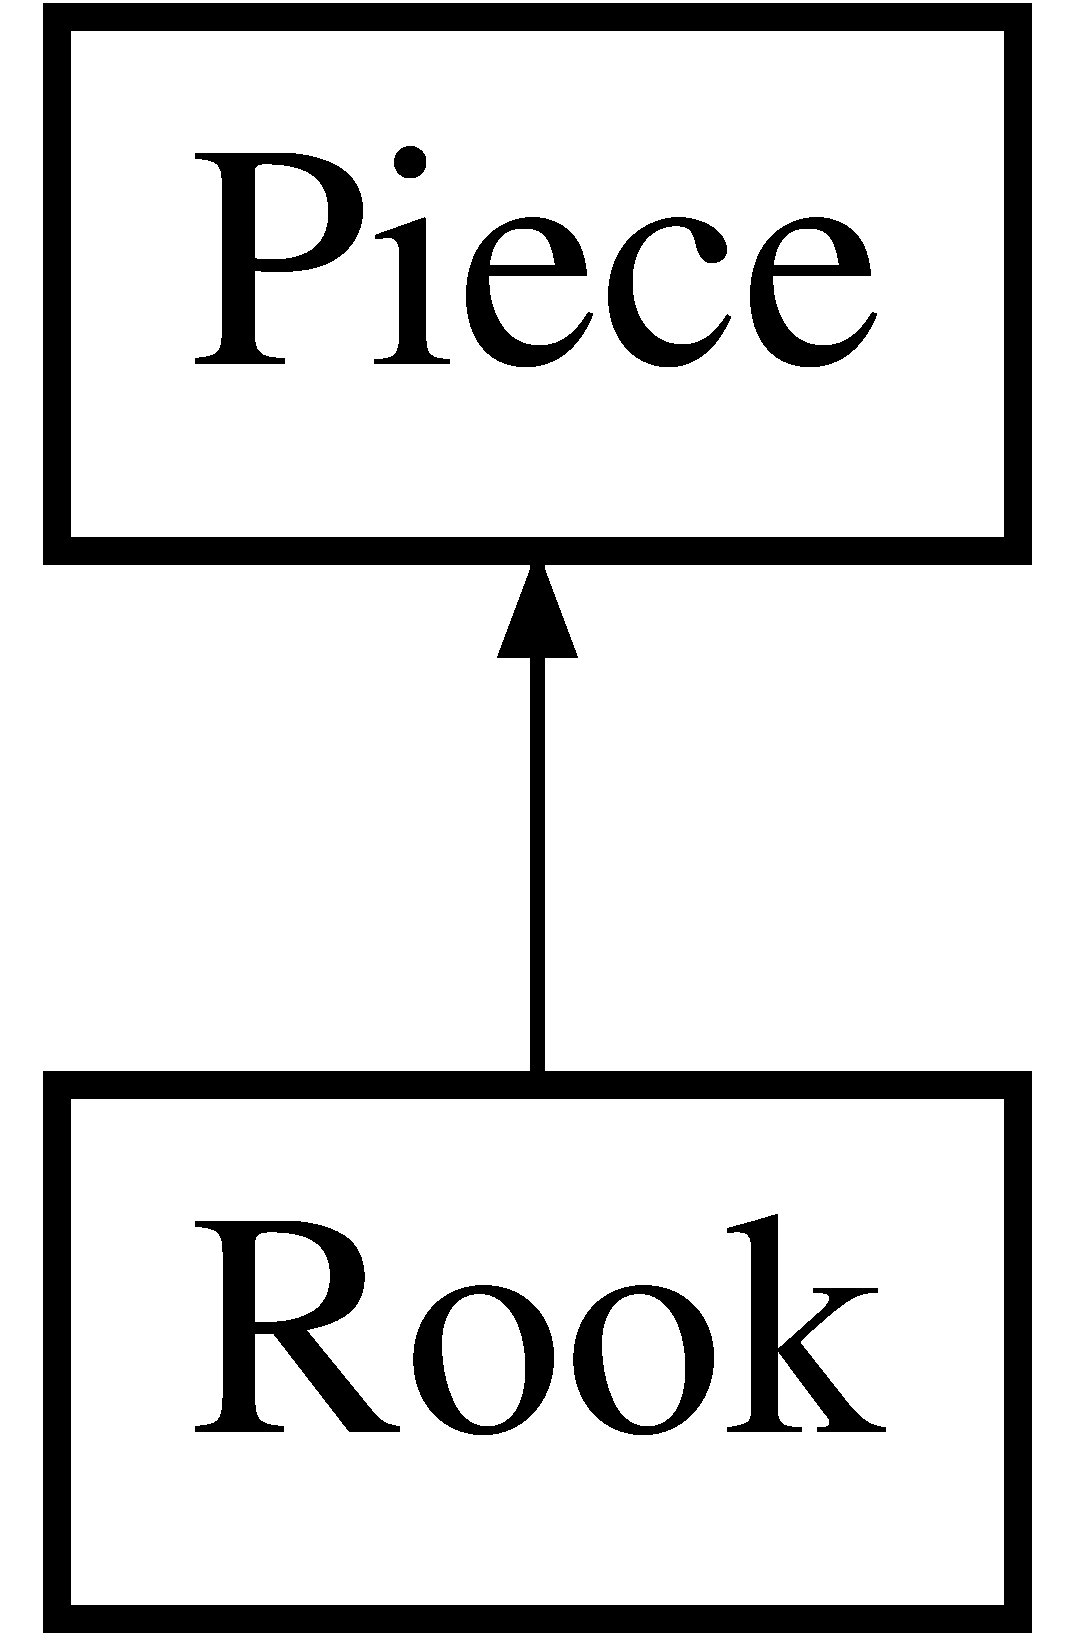
\includegraphics[height=2.000000cm]{class_rook}
\end{center}
\end{figure}
\subsection*{Fonctions membres publiques}
\begin{DoxyCompactItemize}
\item 
\hyperlink{class_rook_ab9613a93abc8a73bda94c596868ec1b1}{Rook} (unsigned int x, unsigned int y)
\begin{DoxyCompactList}\small\item\em Constructeur, crée un objet \hyperlink{class_rook}{Rook} de coordonnées x,y. \end{DoxyCompactList}\item 
\hyperlink{class_rook_a70d445b94848b22ded850b6f58bc2972}{$\sim$\-Rook} ()
\begin{DoxyCompactList}\small\item\em Destructeur d'un objet \hyperlink{class_rook}{Rook}. \end{DoxyCompactList}\item 
bool \hyperlink{class_rook_afb50e8a85759ba7518b55dace6b6e406}{as\-Moved} ()
\begin{DoxyCompactList}\small\item\em Getter de l'attribut \-\_\-moved. \end{DoxyCompactList}\item 
void \hyperlink{class_rook_a7ee5b6169a3fff6d5536ba0c02607950}{set\-Moved} (bool new\-Moved)
\begin{DoxyCompactList}\small\item\em Setter de l'attribut \-\_\-moved. \end{DoxyCompactList}\item 
virtual void \hyperlink{class_rook_acc6139577c8ca679a93dcfbe42b71cb3}{movement} ()
\begin{DoxyCompactList}\small\item\em procédure virtuelle permettant de mettre à jour l'attribut movements en fonction des déplacements possibles de la Tour \end{DoxyCompactList}\end{DoxyCompactItemize}
\subsection*{Membres hérités additionnels}


\subsection{Description détaillée}
Classe \hyperlink{class_rook}{Rook} héritant de \hyperlink{class_piece}{Piece}. 

\subsection{Documentation des constructeurs et destructeur}
\hypertarget{class_rook_ab9613a93abc8a73bda94c596868ec1b1}{\index{Rook@{Rook}!Rook@{Rook}}
\index{Rook@{Rook}!Rook@{Rook}}
\subsubsection[{Rook}]{\setlength{\rightskip}{0pt plus 5cm}Rook\-::\-Rook (
\begin{DoxyParamCaption}
\item[{unsigned int}]{x, }
\item[{unsigned int}]{y}
\end{DoxyParamCaption}
)}}\label{class_rook_ab9613a93abc8a73bda94c596868ec1b1}


Constructeur, crée un objet \hyperlink{class_rook}{Rook} de coordonnées x,y. 


\begin{DoxyParams}{Paramètres}
{\em unsigned} & int x \\
\hline
{\em unsigned} & int y \\
\hline
\end{DoxyParams}
\hypertarget{class_rook_a70d445b94848b22ded850b6f58bc2972}{\index{Rook@{Rook}!$\sim$\-Rook@{$\sim$\-Rook}}
\index{$\sim$\-Rook@{$\sim$\-Rook}!Rook@{Rook}}
\subsubsection[{$\sim$\-Rook}]{\setlength{\rightskip}{0pt plus 5cm}Rook\-::$\sim$\-Rook (
\begin{DoxyParamCaption}
{}
\end{DoxyParamCaption}
)}}\label{class_rook_a70d445b94848b22ded850b6f58bc2972}


Destructeur d'un objet \hyperlink{class_rook}{Rook}. 



\subsection{Documentation des fonctions membres}
\hypertarget{class_rook_afb50e8a85759ba7518b55dace6b6e406}{\index{Rook@{Rook}!as\-Moved@{as\-Moved}}
\index{as\-Moved@{as\-Moved}!Rook@{Rook}}
\subsubsection[{as\-Moved}]{\setlength{\rightskip}{0pt plus 5cm}bool Rook\-::as\-Moved (
\begin{DoxyParamCaption}
{}
\end{DoxyParamCaption}
)}}\label{class_rook_afb50e8a85759ba7518b55dace6b6e406}


Getter de l'attribut \-\_\-moved. 

\begin{DoxyReturn}{Renvoie}
attribut \-\_\-moved 
\end{DoxyReturn}
\hypertarget{class_rook_acc6139577c8ca679a93dcfbe42b71cb3}{\index{Rook@{Rook}!movement@{movement}}
\index{movement@{movement}!Rook@{Rook}}
\subsubsection[{movement}]{\setlength{\rightskip}{0pt plus 5cm}void Rook\-::movement (
\begin{DoxyParamCaption}
{}
\end{DoxyParamCaption}
)\hspace{0.3cm}{\ttfamily [virtual]}}}\label{class_rook_acc6139577c8ca679a93dcfbe42b71cb3}


procédure virtuelle permettant de mettre à jour l'attribut movements en fonction des déplacements possibles de la Tour 



Réimplémentée à partir de \hyperlink{class_piece_ae721b5ed94376fd4e7d348d36739ed4d}{Piece}.

\hypertarget{class_rook_a7ee5b6169a3fff6d5536ba0c02607950}{\index{Rook@{Rook}!set\-Moved@{set\-Moved}}
\index{set\-Moved@{set\-Moved}!Rook@{Rook}}
\subsubsection[{set\-Moved}]{\setlength{\rightskip}{0pt plus 5cm}void Rook\-::set\-Moved (
\begin{DoxyParamCaption}
\item[{bool}]{new\-Moved}
\end{DoxyParamCaption}
)}}\label{class_rook_a7ee5b6169a3fff6d5536ba0c02607950}


Setter de l'attribut \-\_\-moved. 


\begin{DoxyParams}{Paramètres}
{\em bool} & new\-Moved \\
\hline
\end{DoxyParams}


La documentation de cette classe a été générée à partir des fichiers suivants \-:\begin{DoxyCompactItemize}
\item 
src/\hyperlink{_piece_8hpp}{Piece.\-hpp}\item 
src/\hyperlink{_piece_8cpp}{Piece.\-cpp}\end{DoxyCompactItemize}

\hypertarget{class_spawn}{\section{Référence de la classe Spawn}
\label{class_spawn}\index{Spawn@{Spawn}}
}


Classe \hyperlink{class_spawn}{Spawn} héritant de \hyperlink{class_piece}{Piece}.  




{\ttfamily \#include $<$Piece.\-hpp$>$}

Graphe d'héritage de Spawn\-:\begin{figure}[H]
\begin{center}
\leavevmode
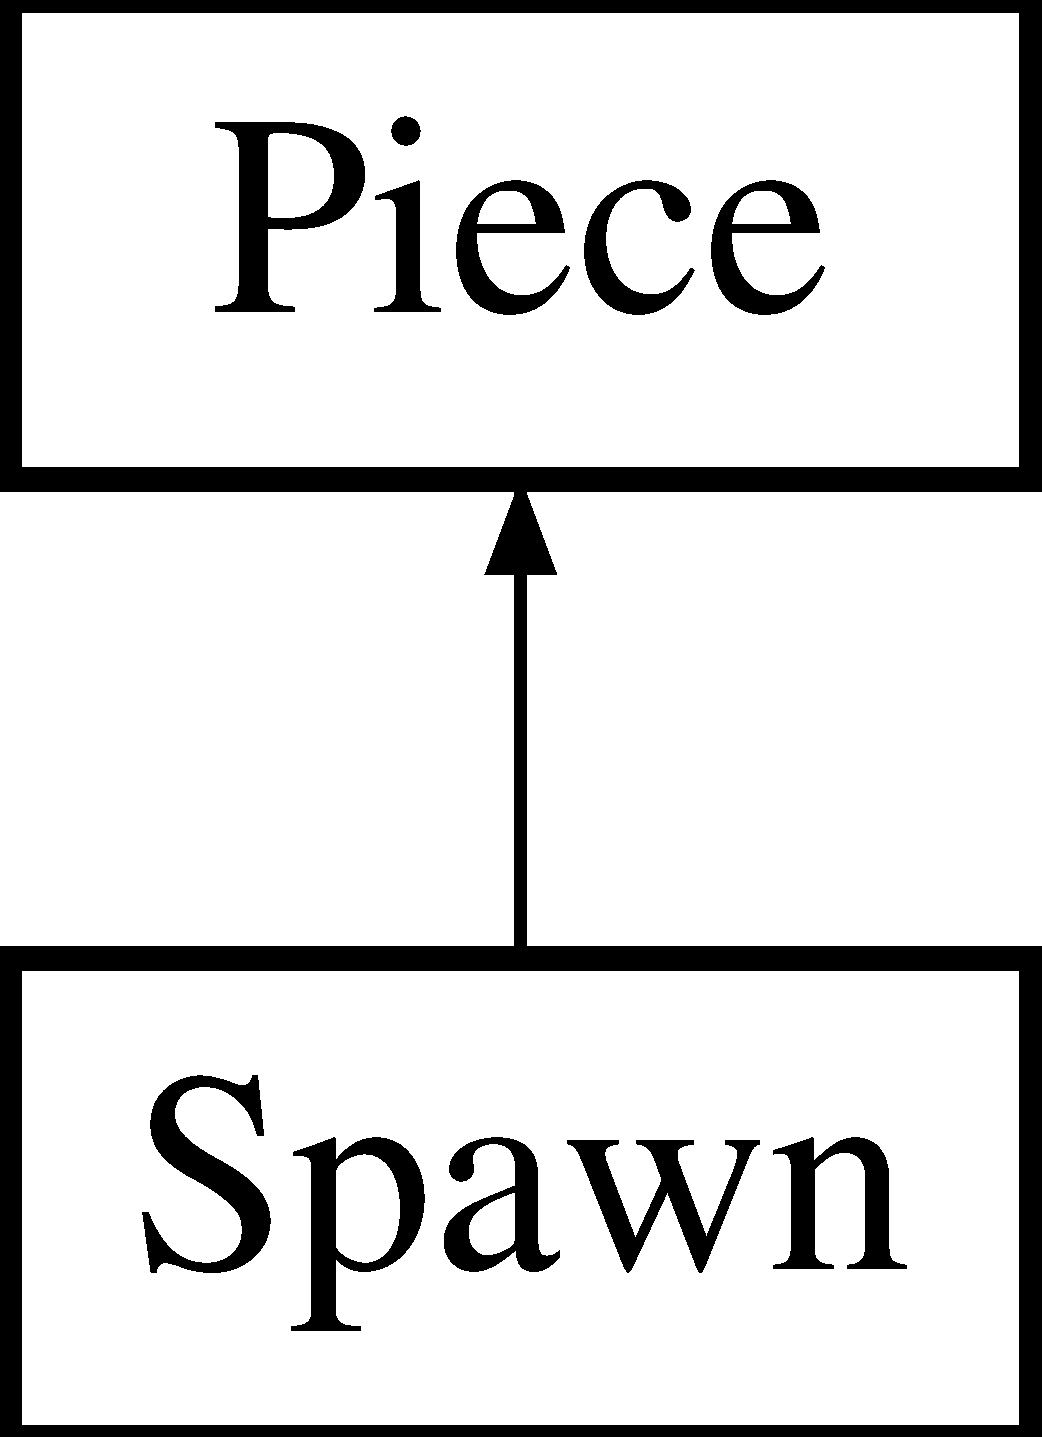
\includegraphics[height=2.000000cm]{class_spawn}
\end{center}
\end{figure}
\subsection*{Fonctions membres publiques}
\begin{DoxyCompactItemize}
\item 
\hyperlink{class_spawn_ad401aa751cbbf9ea4f444e3011ff36b5}{Spawn} (unsigned int x, unsigned int y, bool direction)
\begin{DoxyCompactList}\small\item\em Constructeur, crée un objet \hyperlink{class_spawn}{Spawn} de coordonnées x,y. \end{DoxyCompactList}\item 
\hyperlink{class_spawn_aea08036b23acdb06fd47eba35dc2a8cf}{$\sim$\-Spawn} ()
\begin{DoxyCompactList}\small\item\em Destructeur d'un objet cavalier. \end{DoxyCompactList}\item 
virtual void \hyperlink{class_spawn_ae176dffa40411480840c3e39cd619300}{movement} ()
\begin{DoxyCompactList}\small\item\em procédure virtuelle permettant de mettre à jour l'attribut movements en fonction des déplacements possibles du Pion \end{DoxyCompactList}\end{DoxyCompactItemize}
\subsection*{Membres hérités additionnels}


\subsection{Description détaillée}
Classe \hyperlink{class_spawn}{Spawn} héritant de \hyperlink{class_piece}{Piece}. 

\subsection{Documentation des constructeurs et destructeur}
\hypertarget{class_spawn_ad401aa751cbbf9ea4f444e3011ff36b5}{\index{Spawn@{Spawn}!Spawn@{Spawn}}
\index{Spawn@{Spawn}!Spawn@{Spawn}}
\subsubsection[{Spawn}]{\setlength{\rightskip}{0pt plus 5cm}Spawn\-::\-Spawn (
\begin{DoxyParamCaption}
\item[{unsigned int}]{x, }
\item[{unsigned int}]{y, }
\item[{bool}]{direction}
\end{DoxyParamCaption}
)}}\label{class_spawn_ad401aa751cbbf9ea4f444e3011ff36b5}


Constructeur, crée un objet \hyperlink{class_spawn}{Spawn} de coordonnées x,y. 


\begin{DoxyParams}{Paramètres}
{\em unsigned} & int x \\
\hline
{\em unsigned} & int y \\
\hline
{\em bool} & haut(true)/bas(false) \\
\hline
\end{DoxyParams}
\hypertarget{class_spawn_aea08036b23acdb06fd47eba35dc2a8cf}{\index{Spawn@{Spawn}!$\sim$\-Spawn@{$\sim$\-Spawn}}
\index{$\sim$\-Spawn@{$\sim$\-Spawn}!Spawn@{Spawn}}
\subsubsection[{$\sim$\-Spawn}]{\setlength{\rightskip}{0pt plus 5cm}Spawn\-::$\sim$\-Spawn (
\begin{DoxyParamCaption}
{}
\end{DoxyParamCaption}
)}}\label{class_spawn_aea08036b23acdb06fd47eba35dc2a8cf}


Destructeur d'un objet cavalier. 



\subsection{Documentation des fonctions membres}
\hypertarget{class_spawn_ae176dffa40411480840c3e39cd619300}{\index{Spawn@{Spawn}!movement@{movement}}
\index{movement@{movement}!Spawn@{Spawn}}
\subsubsection[{movement}]{\setlength{\rightskip}{0pt plus 5cm}void Spawn\-::movement (
\begin{DoxyParamCaption}
{}
\end{DoxyParamCaption}
)\hspace{0.3cm}{\ttfamily [virtual]}}}\label{class_spawn_ae176dffa40411480840c3e39cd619300}


procédure virtuelle permettant de mettre à jour l'attribut movements en fonction des déplacements possibles du Pion 



Réimplémentée à partir de \hyperlink{class_piece_ae721b5ed94376fd4e7d348d36739ed4d}{Piece}.



La documentation de cette classe a été générée à partir des fichiers suivants \-:\begin{DoxyCompactItemize}
\item 
src/\hyperlink{_piece_8hpp}{Piece.\-hpp}\item 
src/\hyperlink{_piece_8cpp}{Piece.\-cpp}\end{DoxyCompactItemize}

\hypertarget{class_state}{\section{Référence de la classe State}
\label{class_state}\index{State@{State}}
}


{\ttfamily \#include $<$State.\-hpp$>$}

Graphe d'héritage de State\-:\begin{figure}[H]
\begin{center}
\leavevmode
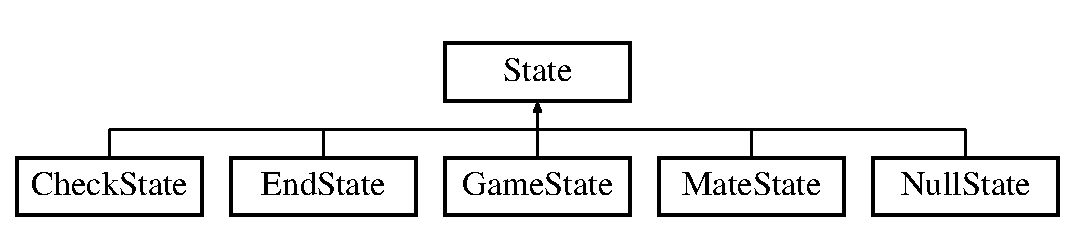
\includegraphics[height=2.000000cm]{class_state}
\end{center}
\end{figure}
\subsection*{Fonctions membres publiques}
\begin{DoxyCompactItemize}
\item 
\hyperlink{class_state_a7a0a6af0cd97aa575a097eca87e090ba}{State} (\hyperlink{class_player}{Player} $\ast$p)
\begin{DoxyCompactList}\small\item\em Constructeur, crée un Etat avec un Joueur en paramètre. \end{DoxyCompactList}\item 
\hyperlink{class_state_afab438d92b90dc18d194dbd9c9c8bab3}{$\sim$\-State} ()
\begin{DoxyCompactList}\small\item\em Destructeur de l'objet \hyperlink{class_state}{State}. \end{DoxyCompactList}\item 
virtual void \hyperlink{class_state_a738b04d6e0c12a39bf96a2a7159202d8}{in\-Game} ()=0
\begin{DoxyCompactList}\small\item\em procédure virtuelle permettant de la transition de l'état \hyperlink{class_check_state}{Check\-State} à l'état \hyperlink{class_game_state}{Game\-State} \end{DoxyCompactList}\item 
virtual void \hyperlink{class_state_a321fd726bbefc35fedbbf001d2a37021}{check} ()=0
\begin{DoxyCompactList}\small\item\em procédure virtuelle permettant de la transition de l'état \hyperlink{class_game_state}{Game\-State} à l'état \hyperlink{class_check_state}{Check\-State} \end{DoxyCompactList}\item 
virtual void \hyperlink{class_state_aa2b89ec92ecd4f6271269fe4b8ccc790}{check\-Mate} ()=0
\begin{DoxyCompactList}\small\item\em procédure virtuelle permettant de la transition de l'état \hyperlink{class_game_state}{Game\-State} à l'état \hyperlink{class_mate_state}{Mate\-State} \end{DoxyCompactList}\item 
virtual void \hyperlink{class_state_ad5b7fe10b2c30243f36d7d0950c50d43}{game\-Null} ()=0
\begin{DoxyCompactList}\small\item\em procédure virtuelle permettant de la transition de l'état \hyperlink{class_game_state}{Game\-State} à l'état \hyperlink{class_null_state}{Null\-State} \end{DoxyCompactList}\item 
virtual void \hyperlink{class_state_a5117e1f9bf06e17b4b0277838fe39bd8}{game\-End} ()=0
\begin{DoxyCompactList}\small\item\em procédure virtuelle permettant de la transition de l'état \hyperlink{class_mate_state}{Mate\-State} ou l'état \hyperlink{class_null_state}{Null\-State} à l'état \hyperlink{class_end_state}{End\-State} \end{DoxyCompactList}\item 
virtual void \hyperlink{class_state_a95a537bb55b9118b23d5bed88ba3b335}{print} ()=0
\begin{DoxyCompactList}\small\item\em procédure virtuelle permettant d'afficher l'état courant \end{DoxyCompactList}\item 
virtual bool \hyperlink{class_state_ad2d7084c507d8d20be2e772d953129fb}{ischeck} ()=0
\begin{DoxyCompactList}\small\item\em procédure virtuelle permettant de savoir s'il se trouve en possition d'echec \end{DoxyCompactList}\item 
virtual bool \hyperlink{class_state_ae1d813f250db75015ddeebece5ec0f2b}{ischeckmate} ()=0
\begin{DoxyCompactList}\small\item\em procédure virtuelle permettant de savoir s'il se trouve en possition d'echec et mate \end{DoxyCompactList}\item 
virtual bool \hyperlink{class_state_a869f2ebfad7e60719df5f89a613adee1}{isnulle} ()=0
\begin{DoxyCompactList}\small\item\em procédure virtuelle permettant de savoir s'il se trouve en possition null \end{DoxyCompactList}\end{DoxyCompactItemize}
\subsection*{Attributs protégés}
\begin{DoxyCompactItemize}
\item 
\hyperlink{class_player}{Player} $\ast$ \hyperlink{class_state_a9a024fd38161f32fc10b68b4ccb13226}{player}
\end{DoxyCompactItemize}


\subsection{Documentation des constructeurs et destructeur}
\hypertarget{class_state_a7a0a6af0cd97aa575a097eca87e090ba}{\index{State@{State}!State@{State}}
\index{State@{State}!State@{State}}
\subsubsection[{State}]{\setlength{\rightskip}{0pt plus 5cm}State\-::\-State (
\begin{DoxyParamCaption}
\item[{{\bf Player} $\ast$}]{p}
\end{DoxyParamCaption}
)}}\label{class_state_a7a0a6af0cd97aa575a097eca87e090ba}


Constructeur, crée un Etat avec un Joueur en paramètre. 


\begin{DoxyParams}{Paramètres}
{\em p} & \\
\hline
\end{DoxyParams}
\hypertarget{class_state_afab438d92b90dc18d194dbd9c9c8bab3}{\index{State@{State}!$\sim$\-State@{$\sim$\-State}}
\index{$\sim$\-State@{$\sim$\-State}!State@{State}}
\subsubsection[{$\sim$\-State}]{\setlength{\rightskip}{0pt plus 5cm}State\-::$\sim$\-State (
\begin{DoxyParamCaption}
{}
\end{DoxyParamCaption}
)}}\label{class_state_afab438d92b90dc18d194dbd9c9c8bab3}


Destructeur de l'objet \hyperlink{class_state}{State}. 



\subsection{Documentation des fonctions membres}
\hypertarget{class_state_a321fd726bbefc35fedbbf001d2a37021}{\index{State@{State}!check@{check}}
\index{check@{check}!State@{State}}
\subsubsection[{check}]{\setlength{\rightskip}{0pt plus 5cm}void State\-::check (
\begin{DoxyParamCaption}
{}
\end{DoxyParamCaption}
)\hspace{0.3cm}{\ttfamily [pure virtual]}}}\label{class_state_a321fd726bbefc35fedbbf001d2a37021}


procédure virtuelle permettant de la transition de l'état \hyperlink{class_game_state}{Game\-State} à l'état \hyperlink{class_check_state}{Check\-State} 



Implémenté dans \hyperlink{class_end_state_a80e538c38c1293803200e5d3b513ba77}{End\-State}, \hyperlink{class_null_state_a04825452cd1018dec2525609a3079aff}{Null\-State}, \hyperlink{class_mate_state_a2205b5879c63fcdf469002d9d5203bb3}{Mate\-State}, \hyperlink{class_check_state_a7e365f95e322b61609f05202c28db278}{Check\-State}, et \hyperlink{class_game_state_a646e5436c4191f323dfa736a06e79695}{Game\-State}.

\hypertarget{class_state_aa2b89ec92ecd4f6271269fe4b8ccc790}{\index{State@{State}!check\-Mate@{check\-Mate}}
\index{check\-Mate@{check\-Mate}!State@{State}}
\subsubsection[{check\-Mate}]{\setlength{\rightskip}{0pt plus 5cm}void State\-::check\-Mate (
\begin{DoxyParamCaption}
{}
\end{DoxyParamCaption}
)\hspace{0.3cm}{\ttfamily [pure virtual]}}}\label{class_state_aa2b89ec92ecd4f6271269fe4b8ccc790}


procédure virtuelle permettant de la transition de l'état \hyperlink{class_game_state}{Game\-State} à l'état \hyperlink{class_mate_state}{Mate\-State} 



Implémenté dans \hyperlink{class_end_state_a48a2531ee4bd2144b44823a5527488f3}{End\-State}, \hyperlink{class_null_state_a2bc6da41f64658fb9f733f6b23f0e499}{Null\-State}, \hyperlink{class_mate_state_af785a3407109dd3d0a6868a358c92213}{Mate\-State}, \hyperlink{class_check_state_afb093377619bc04bcba50db601368019}{Check\-State}, et \hyperlink{class_game_state_ada8cd91a048922c4d8aedbef17ce6fbc}{Game\-State}.

\hypertarget{class_state_a5117e1f9bf06e17b4b0277838fe39bd8}{\index{State@{State}!game\-End@{game\-End}}
\index{game\-End@{game\-End}!State@{State}}
\subsubsection[{game\-End}]{\setlength{\rightskip}{0pt plus 5cm}void State\-::game\-End (
\begin{DoxyParamCaption}
{}
\end{DoxyParamCaption}
)\hspace{0.3cm}{\ttfamily [pure virtual]}}}\label{class_state_a5117e1f9bf06e17b4b0277838fe39bd8}


procédure virtuelle permettant de la transition de l'état \hyperlink{class_mate_state}{Mate\-State} ou l'état \hyperlink{class_null_state}{Null\-State} à l'état \hyperlink{class_end_state}{End\-State} 



Implémenté dans \hyperlink{class_end_state_a6fc13eb28853a79e1b5396dd2f377a51}{End\-State}, \hyperlink{class_null_state_a73b1449815c3770ac24e56fa885a7961}{Null\-State}, \hyperlink{class_mate_state_a19b4fa2115a36da6e1dd333a617ee7bb}{Mate\-State}, \hyperlink{class_check_state_a54820bb890cc50e3782104fad094747f}{Check\-State}, et \hyperlink{class_game_state_a65fc1ef481baa95f675ff8a78aa14e05}{Game\-State}.

\hypertarget{class_state_ad5b7fe10b2c30243f36d7d0950c50d43}{\index{State@{State}!game\-Null@{game\-Null}}
\index{game\-Null@{game\-Null}!State@{State}}
\subsubsection[{game\-Null}]{\setlength{\rightskip}{0pt plus 5cm}void State\-::game\-Null (
\begin{DoxyParamCaption}
{}
\end{DoxyParamCaption}
)\hspace{0.3cm}{\ttfamily [pure virtual]}}}\label{class_state_ad5b7fe10b2c30243f36d7d0950c50d43}


procédure virtuelle permettant de la transition de l'état \hyperlink{class_game_state}{Game\-State} à l'état \hyperlink{class_null_state}{Null\-State} 



Implémenté dans \hyperlink{class_end_state_ad50c108e27c7b0497c3f2f2e76b904a5}{End\-State}, \hyperlink{class_null_state_a9a735f7e4cbf7c3439208f9bb90b649d}{Null\-State}, \hyperlink{class_mate_state_a59ad17cb3366c560b921619d52f00181}{Mate\-State}, \hyperlink{class_check_state_ae3cc6446e2dd5de333797bb180104c50}{Check\-State}, et \hyperlink{class_game_state_a006f729bc30cfa224d3235c87e5a6e59}{Game\-State}.

\hypertarget{class_state_a738b04d6e0c12a39bf96a2a7159202d8}{\index{State@{State}!in\-Game@{in\-Game}}
\index{in\-Game@{in\-Game}!State@{State}}
\subsubsection[{in\-Game}]{\setlength{\rightskip}{0pt plus 5cm}void State\-::in\-Game (
\begin{DoxyParamCaption}
{}
\end{DoxyParamCaption}
)\hspace{0.3cm}{\ttfamily [pure virtual]}}}\label{class_state_a738b04d6e0c12a39bf96a2a7159202d8}


procédure virtuelle permettant de la transition de l'état \hyperlink{class_check_state}{Check\-State} à l'état \hyperlink{class_game_state}{Game\-State} 



Implémenté dans \hyperlink{class_end_state_a6ba5aa5cfd2d0ac4aa1609e336d5669f}{End\-State}, \hyperlink{class_null_state_a3c51a85d1d0273b7f7db4ed20672c68c}{Null\-State}, \hyperlink{class_mate_state_a99575ed4587f029511bc5bd1ec9ab262}{Mate\-State}, \hyperlink{class_check_state_a3cc0cb64d061a72d91ee60b60801aa3b}{Check\-State}, et \hyperlink{class_game_state_af0290fd87a2bc2a44119dc700d8b8721}{Game\-State}.

\hypertarget{class_state_ad2d7084c507d8d20be2e772d953129fb}{\index{State@{State}!ischeck@{ischeck}}
\index{ischeck@{ischeck}!State@{State}}
\subsubsection[{ischeck}]{\setlength{\rightskip}{0pt plus 5cm}bool State\-::ischeck (
\begin{DoxyParamCaption}
{}
\end{DoxyParamCaption}
)\hspace{0.3cm}{\ttfamily [pure virtual]}}}\label{class_state_ad2d7084c507d8d20be2e772d953129fb}


procédure virtuelle permettant de savoir s'il se trouve en possition d'echec 



Implémenté dans \hyperlink{class_end_state_ae4ea53e0246be8cf37ccd8cf7b442523}{End\-State}, \hyperlink{class_null_state_a8da9c3d889ff161f893d5522a89567a5}{Null\-State}, \hyperlink{class_mate_state_a47e7642586f54efaa977755bb2b2311d}{Mate\-State}, \hyperlink{class_check_state_aa6e88c453114883d8a415ff338b65526}{Check\-State}, et \hyperlink{class_game_state_ae0f8b04f85ed4dfbbd4c2a6a06827273}{Game\-State}.

\hypertarget{class_state_ae1d813f250db75015ddeebece5ec0f2b}{\index{State@{State}!ischeckmate@{ischeckmate}}
\index{ischeckmate@{ischeckmate}!State@{State}}
\subsubsection[{ischeckmate}]{\setlength{\rightskip}{0pt plus 5cm}bool State\-::ischeckmate (
\begin{DoxyParamCaption}
{}
\end{DoxyParamCaption}
)\hspace{0.3cm}{\ttfamily [pure virtual]}}}\label{class_state_ae1d813f250db75015ddeebece5ec0f2b}


procédure virtuelle permettant de savoir s'il se trouve en possition d'echec et mate 



Implémenté dans \hyperlink{class_end_state_a2f505cd7004247548a3026ce70bc0f58}{End\-State}, \hyperlink{class_null_state_adda1a19059bc77cf09886873912f91ff}{Null\-State}, \hyperlink{class_mate_state_a9b9eb5923dc94adb69b28174d580c3b1}{Mate\-State}, \hyperlink{class_check_state_ae3704aaa5fbaf6c947462c211eafc9c9}{Check\-State}, et \hyperlink{class_game_state_a595eb9db47758b91835fc12b13311b98}{Game\-State}.

\hypertarget{class_state_a869f2ebfad7e60719df5f89a613adee1}{\index{State@{State}!isnulle@{isnulle}}
\index{isnulle@{isnulle}!State@{State}}
\subsubsection[{isnulle}]{\setlength{\rightskip}{0pt plus 5cm}bool State\-::isnulle (
\begin{DoxyParamCaption}
{}
\end{DoxyParamCaption}
)\hspace{0.3cm}{\ttfamily [pure virtual]}}}\label{class_state_a869f2ebfad7e60719df5f89a613adee1}


procédure virtuelle permettant de savoir s'il se trouve en possition null 



Implémenté dans \hyperlink{class_end_state_aa9ccf089beda25f9d258e6a68e2a7309}{End\-State}, \hyperlink{class_null_state_a0aa0845d4f2ce4f86749bd73edb8c8da}{Null\-State}, \hyperlink{class_mate_state_a0d586f9c4dafd94ebfa6b14e425fff8b}{Mate\-State}, \hyperlink{class_check_state_a569daf96d0340272068a3d36fdf288c4}{Check\-State}, et \hyperlink{class_game_state_a777e982cbef6125ba4003f68d6292825}{Game\-State}.

\hypertarget{class_state_a95a537bb55b9118b23d5bed88ba3b335}{\index{State@{State}!print@{print}}
\index{print@{print}!State@{State}}
\subsubsection[{print}]{\setlength{\rightskip}{0pt plus 5cm}void State\-::print (
\begin{DoxyParamCaption}
{}
\end{DoxyParamCaption}
)\hspace{0.3cm}{\ttfamily [pure virtual]}}}\label{class_state_a95a537bb55b9118b23d5bed88ba3b335}


procédure virtuelle permettant d'afficher l'état courant 



Implémenté dans \hyperlink{class_end_state_a1983377ed8a1e391871fb40db39f13e3}{End\-State}, \hyperlink{class_null_state_a5a2b2f419bba204759bf344c8b7710d0}{Null\-State}, \hyperlink{class_mate_state_ab96d11c6cbb289483659d55bb8735c77}{Mate\-State}, \hyperlink{class_check_state_ace4965a79b3614c50d0db5396121b75e}{Check\-State}, et \hyperlink{class_game_state_a9ccc5473c6f04e60711cb9a438b276e5}{Game\-State}.



\subsection{Documentation des données membres}
\hypertarget{class_state_a9a024fd38161f32fc10b68b4ccb13226}{\index{State@{State}!player@{player}}
\index{player@{player}!State@{State}}
\subsubsection[{player}]{\setlength{\rightskip}{0pt plus 5cm}{\bf Player}$\ast$ State\-::player\hspace{0.3cm}{\ttfamily [protected]}}}\label{class_state_a9a024fd38161f32fc10b68b4ccb13226}


La documentation de cette classe a été générée à partir des fichiers suivants \-:\begin{DoxyCompactItemize}
\item 
src/\hyperlink{_state_8hpp}{State.\-hpp}\item 
src/\hyperlink{_state_8cpp}{State.\-cpp}\end{DoxyCompactItemize}

\input{class_team}
\chapter{Documentation des fichiers}
\hypertarget{_r_e_a_d_m_e_8md}{\section{Référence du fichier R\-E\-A\-D\-M\-E.\-md}
\label{_r_e_a_d_m_e_8md}\index{R\-E\-A\-D\-M\-E.\-md@{R\-E\-A\-D\-M\-E.\-md}}
}

\hypertarget{_cell_8cpp}{\section{Référence du fichier src/\-Cell.cpp}
\label{_cell_8cpp}\index{src/\-Cell.\-cpp@{src/\-Cell.\-cpp}}
}


implémentation des méthodes de la classe \hyperlink{class_cell}{Cell}  


{\ttfamily \#include \char`\"{}Cell.\-hpp\char`\"{}}\\*


\subsection{Description détaillée}
implémentation des méthodes de la classe \hyperlink{class_cell}{Cell} \begin{DoxyAuthor}{Auteur}
P. Sullivan, G.\-Laurent 
\end{DoxyAuthor}
\begin{DoxySince}{Depuis}
25/12/2015 
\end{DoxySince}

\hypertarget{_cell_8hpp}{\section{Référence du fichier src/\-Cell.hpp}
\label{_cell_8hpp}\index{src/\-Cell.\-hpp@{src/\-Cell.\-hpp}}
}


Définition d'une classe de \hyperlink{class_cell}{Cell}.  


{\ttfamily \#include $<$iostream$>$}\\*
\subsection*{Classes}
\begin{DoxyCompactItemize}
\item 
class \hyperlink{class_cell}{Cell}
\begin{DoxyCompactList}\small\item\em Classe permettant de représenter une case du jeu d'echec. \end{DoxyCompactList}\end{DoxyCompactItemize}


\subsection{Description détaillée}
Définition d'une classe de \hyperlink{class_cell}{Cell}. \begin{DoxyAuthor}{Auteur}
P. Sullivan, G.\-Laurent 
\end{DoxyAuthor}
\begin{DoxySince}{Depuis}
25/12/2015 
\end{DoxySince}

\hypertarget{_chess_8cpp}{\section{Référence du fichier src/\-Chess.cpp}
\label{_chess_8cpp}\index{src/\-Chess.\-cpp@{src/\-Chess.\-cpp}}
}


implémentation des méthodes de la classe \hyperlink{class_chess}{Chess}  


{\ttfamily \#include \char`\"{}Chess.\-hpp\char`\"{}}\\*


\subsection{Description détaillée}
implémentation des méthodes de la classe \hyperlink{class_chess}{Chess} \begin{DoxyAuthor}{Auteur}
P. Sullivan, G.\-Laurent 
\end{DoxyAuthor}
\begin{DoxySince}{Depuis}
25/12/2015 
\end{DoxySince}

\hypertarget{_chess_8hpp}{\section{Référence du fichier src/\-Chess.hpp}
\label{_chess_8hpp}\index{src/\-Chess.\-hpp@{src/\-Chess.\-hpp}}
}


Définition de la classe \hyperlink{class_chess}{Chess}, permettant aux deux joueurs d'intéragir sur le plateau.  


{\ttfamily \#include \char`\"{}Player.\-hpp\char`\"{}}\\*
\subsection*{Classes}
\begin{DoxyCompactItemize}
\item 
class \hyperlink{class_chess}{Chess}
\end{DoxyCompactItemize}


\subsection{Description détaillée}
Définition de la classe \hyperlink{class_chess}{Chess}, permettant aux deux joueurs d'intéragir sur le plateau. \begin{DoxyAuthor}{Auteur}
P. Sullivan, G.\-Laurent 
\end{DoxyAuthor}
\begin{DoxySince}{Depuis}
25/12/2015 
\end{DoxySince}

\hypertarget{_factory_8cpp}{\section{Référence du fichier src/\-Factory.cpp}
\label{_factory_8cpp}\index{src/\-Factory.\-cpp@{src/\-Factory.\-cpp}}
}
{\ttfamily \#include \char`\"{}Factory.\-hpp\char`\"{}}\\*

\hypertarget{_factory_8hpp}{\section{Référence du fichier src/\-Factory.hpp}
\label{_factory_8hpp}\index{src/\-Factory.\-hpp@{src/\-Factory.\-hpp}}
}


Définition de la factoty.  


{\ttfamily \#include \char`\"{}Piece.\-hpp\char`\"{}}\\*
\subsection*{Classes}
\begin{DoxyCompactItemize}
\item 
class \hyperlink{class_factory}{Factory}
\item 
class \hyperlink{class_factory_spawn}{Factory\-Spawn}
\begin{DoxyCompactList}\small\item\em Classe \hyperlink{class_factory_spawn}{Factory\-Spawn} héritant de \hyperlink{class_factory}{Factory}. \end{DoxyCompactList}\item 
class \hyperlink{class_factory_rook}{Factory\-Rook}
\begin{DoxyCompactList}\small\item\em Classe \hyperlink{class_factory_rook}{Factory\-Rook} héritant de \hyperlink{class_factory}{Factory}. \end{DoxyCompactList}\item 
class \hyperlink{class_factory_knight}{Factory\-Knight}
\begin{DoxyCompactList}\small\item\em Classe \hyperlink{class_factory_knight}{Factory\-Knight} héritant de \hyperlink{class_factory}{Factory}. \end{DoxyCompactList}\item 
class \hyperlink{class_factory_bishop}{Factory\-Bishop}
\begin{DoxyCompactList}\small\item\em Classe \hyperlink{class_factory_bishop}{Factory\-Bishop} héritant de \hyperlink{class_factory}{Factory}. \end{DoxyCompactList}\item 
class \hyperlink{class_factory_queen}{Factory\-Queen}
\begin{DoxyCompactList}\small\item\em Classe \hyperlink{class_factory_queen}{Factory\-Queen} héritant de \hyperlink{class_factory}{Factory}. \end{DoxyCompactList}\item 
class \hyperlink{class_factory_king}{Factory\-King}
\begin{DoxyCompactList}\small\item\em Classe \hyperlink{class_factory_king}{Factory\-King} héritant de \hyperlink{class_factory}{Factory}. \end{DoxyCompactList}\end{DoxyCompactItemize}


\subsection{Description détaillée}
Définition de la factoty. \begin{DoxyAuthor}{Auteur}
G.\-Laurent, P. Sullivan 
\end{DoxyAuthor}
\begin{DoxySince}{Depuis}
25/12/2015 
\end{DoxySince}

\hypertarget{_game_8cpp}{\section{Référence du fichier src/\-Game.cpp}
\label{_game_8cpp}\index{src/\-Game.\-cpp@{src/\-Game.\-cpp}}
}
{\ttfamily \#include $<$iostream$>$}\\*
{\ttfamily \#include $<$cstdlib$>$}\\*
{\ttfamily \#include $<$string$>$}\\*
{\ttfamily \#include \char`\"{}Chess.\-hpp\char`\"{}}\\*
\subsection*{Fonctions}
\begin{DoxyCompactItemize}
\item 
int \hyperlink{_game_8cpp_ae66f6b31b5ad750f1fe042a706a4e3d4}{main} ()
\end{DoxyCompactItemize}


\subsection{Documentation des fonctions}
\hypertarget{_game_8cpp_ae66f6b31b5ad750f1fe042a706a4e3d4}{\index{Game.\-cpp@{Game.\-cpp}!main@{main}}
\index{main@{main}!Game.cpp@{Game.\-cpp}}
\subsubsection[{main}]{\setlength{\rightskip}{0pt plus 5cm}int main (
\begin{DoxyParamCaption}
{}
\end{DoxyParamCaption}
)}}\label{_game_8cpp_ae66f6b31b5ad750f1fe042a706a4e3d4}

\hypertarget{_object_pool_8cpp}{\section{Référence du fichier src/\-Object\-Pool.cpp}
\label{_object_pool_8cpp}\index{src/\-Object\-Pool.\-cpp@{src/\-Object\-Pool.\-cpp}}
}


implémentation des méthodes de la classe \hyperlink{class_object_pool}{Object\-Pool}  


{\ttfamily \#include \char`\"{}Object\-Pool.\-hpp\char`\"{}}\\*


\subsection{Description détaillée}
implémentation des méthodes de la classe \hyperlink{class_object_pool}{Object\-Pool} \begin{DoxyAuthor}{Auteur}
P. Sullivan, G.\-Laurent 
\end{DoxyAuthor}
\begin{DoxySince}{Depuis}
25/12/2015 
\end{DoxySince}

\hypertarget{_object_pool_8hpp}{\section{Référence du fichier src/\-Object\-Pool.hpp}
\label{_object_pool_8hpp}\index{src/\-Object\-Pool.\-hpp@{src/\-Object\-Pool.\-hpp}}
}


Définition de la classe \hyperlink{class_object_pool}{Object\-Pool} permettant à un joueur de prendre ou remettre ses pièces depuis une pool.  


{\ttfamily \#include \char`\"{}Piece.\-hpp\char`\"{}}\\*
\subsection*{Classes}
\begin{DoxyCompactItemize}
\item 
class \hyperlink{class_object_pool}{Object\-Pool}
\end{DoxyCompactItemize}


\subsection{Description détaillée}
Définition de la classe \hyperlink{class_object_pool}{Object\-Pool} permettant à un joueur de prendre ou remettre ses pièces depuis une pool. \begin{DoxyAuthor}{Auteur}
P. Sullivan, G.\-Laurent 
\end{DoxyAuthor}
\begin{DoxySince}{Depuis}
25/12/2015 
\end{DoxySince}

\hypertarget{_piece_8cpp}{\section{Référence du fichier src/\-Piece.cpp}
\label{_piece_8cpp}\index{src/\-Piece.\-cpp@{src/\-Piece.\-cpp}}
}


implémentation des méthodes de la classe \hyperlink{class_factory}{Factory}  


{\ttfamily \#include \char`\"{}Piece.\-hpp\char`\"{}}\\*


\subsection{Description détaillée}
implémentation des méthodes de la classe \hyperlink{class_factory}{Factory} implémentation des méthodes de la classe \hyperlink{class_piece}{Piece}

\begin{DoxyAuthor}{Auteur}
P. Sullivan, G.\-Laurent 
\end{DoxyAuthor}
\begin{DoxySince}{Depuis}
25/12/2015 
\end{DoxySince}

\hypertarget{_piece_8hpp}{\section{Référence du fichier src/\-Piece.hpp}
\label{_piece_8hpp}\index{src/\-Piece.\-hpp@{src/\-Piece.\-hpp}}
}


Définition d'une classe de \hyperlink{class_piece}{Piece}.  


{\ttfamily \#include \char`\"{}Cell.\-hpp\char`\"{}}\\*
{\ttfamily \#include $<$vector$>$}\\*
{\ttfamily \#include $<$string$>$}\\*
\subsection*{Classes}
\begin{DoxyCompactItemize}
\item 
class \hyperlink{class_piece}{Piece}
\begin{DoxyCompactList}\small\item\em Classe abstaite de \hyperlink{class_piece}{Piece}. \end{DoxyCompactList}\item 
class \hyperlink{class_spawn}{Spawn}
\begin{DoxyCompactList}\small\item\em Classe \hyperlink{class_spawn}{Spawn} héritant de \hyperlink{class_piece}{Piece}. \end{DoxyCompactList}\item 
class \hyperlink{class_rook}{Rook}
\begin{DoxyCompactList}\small\item\em Classe \hyperlink{class_rook}{Rook} héritant de \hyperlink{class_piece}{Piece}. \end{DoxyCompactList}\item 
class \hyperlink{class_knight}{Knight}
\begin{DoxyCompactList}\small\item\em Classe \hyperlink{class_knight}{Knight} héritant de \hyperlink{class_piece}{Piece}. \end{DoxyCompactList}\item 
class \hyperlink{class_bishop}{Bishop}
\begin{DoxyCompactList}\small\item\em Classe \hyperlink{class_bishop}{Bishop} héritant de \hyperlink{class_piece}{Piece}. \end{DoxyCompactList}\item 
class \hyperlink{class_queen}{Queen}
\begin{DoxyCompactList}\small\item\em Classe \hyperlink{class_queen}{Queen} héritant de \hyperlink{class_piece}{Piece}. \end{DoxyCompactList}\item 
class \hyperlink{class_king}{King}
\begin{DoxyCompactList}\small\item\em Classe \hyperlink{class_king}{King} héritant de \hyperlink{class_piece}{Piece}. \end{DoxyCompactList}\end{DoxyCompactItemize}


\subsection{Description détaillée}
Définition d'une classe de \hyperlink{class_piece}{Piece}. \begin{DoxyAuthor}{Auteur}
P. Sullivan, G.\-Laurent 
\end{DoxyAuthor}
\begin{DoxySince}{Depuis}
25/12/2015 
\end{DoxySince}

\hypertarget{_player_8cpp}{\section{Référence du fichier src/\-Player.cpp}
\label{_player_8cpp}\index{src/\-Player.\-cpp@{src/\-Player.\-cpp}}
}


implémentation des méthodes de la classe \hyperlink{class_player}{Player}  


{\ttfamily \#include \char`\"{}Player.\-hpp\char`\"{}}\\*


\subsection{Description détaillée}
implémentation des méthodes de la classe \hyperlink{class_player}{Player} \begin{DoxyAuthor}{Auteur}
P. Sullivan, G.\-Laurent 
\end{DoxyAuthor}
\begin{DoxySince}{Depuis}
25/12/2015 
\end{DoxySince}

\hypertarget{_player_8hpp}{\section{Référence du fichier src/\-Player.hpp}
\label{_player_8hpp}\index{src/\-Player.\-hpp@{src/\-Player.\-hpp}}
}


Définition de la classe \hyperlink{class_player}{Player}.  


{\ttfamily \#include \char`\"{}State.\-hpp\char`\"{}}\\*
{\ttfamily \#include \char`\"{}Piece.\-hpp\char`\"{}}\\*
{\ttfamily \#include \char`\"{}Object\-Pool.\-hpp\char`\"{}}\\*
{\ttfamily \#include \char`\"{}Team.\-hpp\char`\"{}}\\*
\subsection*{Classes}
\begin{DoxyCompactItemize}
\item 
class \hyperlink{class_player}{Player}
\end{DoxyCompactItemize}


\subsection{Description détaillée}
Définition de la classe \hyperlink{class_player}{Player}. \begin{DoxyAuthor}{Auteur}
P. Sullivan, G.\-Laurent 
\end{DoxyAuthor}
\begin{DoxySince}{Depuis}
25/12/2015 
\end{DoxySince}

\hypertarget{_state_8cpp}{\section{Référence du fichier src/\-State.cpp}
\label{_state_8cpp}\index{src/\-State.\-cpp@{src/\-State.\-cpp}}
}


implémentation des méthodes de la classe \hyperlink{class_state}{State} ainsi que de ses classes filles  


{\ttfamily \#include \char`\"{}State.\-hpp\char`\"{}}\\*
{\ttfamily \#include \char`\"{}Player.\-hpp\char`\"{}}\\*


\subsection{Description détaillée}
implémentation des méthodes de la classe \hyperlink{class_state}{State} ainsi que de ses classes filles \begin{DoxyAuthor}{Auteur}
P. Sullivan, G.\-Laurent 
\end{DoxyAuthor}
\begin{DoxySince}{Depuis}
25/12/2015 
\end{DoxySince}

\hypertarget{_state_8hpp}{\section{Référence du fichier src/\-State.hpp}
\label{_state_8hpp}\index{src/\-State.\-hpp@{src/\-State.\-hpp}}
}


Définition de la classe abstraite \hyperlink{class_state}{State} et de ses classes filles (\hyperlink{class_game_state}{Game\-State}, \hyperlink{class_check_state}{Check\-State}, \hyperlink{class_mate_state}{Mate\-State}, \hyperlink{class_null_state}{Null\-State} et \hyperlink{class_end_state}{End\-State})  


\subsection*{Classes}
\begin{DoxyCompactItemize}
\item 
class \hyperlink{class_state}{State}
\item 
class \hyperlink{class_game_state}{Game\-State}
\item 
class \hyperlink{class_check_state}{Check\-State}
\item 
class \hyperlink{class_mate_state}{Mate\-State}
\item 
class \hyperlink{class_null_state}{Null\-State}
\item 
class \hyperlink{class_end_state}{End\-State}
\end{DoxyCompactItemize}


\subsection{Description détaillée}
Définition de la classe abstraite \hyperlink{class_state}{State} et de ses classes filles (\hyperlink{class_game_state}{Game\-State}, \hyperlink{class_check_state}{Check\-State}, \hyperlink{class_mate_state}{Mate\-State}, \hyperlink{class_null_state}{Null\-State} et \hyperlink{class_end_state}{End\-State}) \begin{DoxyAuthor}{Auteur}
P. Sullivan, G.\-Laurent 
\end{DoxyAuthor}
\begin{DoxySince}{Depuis}
25/12/2015 
\end{DoxySince}

\input{_team_8cpp}
\input{_team_8hpp}
%--- End generated contents ---

% Index
\newpage
\phantomsection
\addcontentsline{toc}{chapter}{Index}
\printindex

\end{document}
